%%%%%%%%%%%%%%%%%%%%%%%%%%%%%%%%%%%%%%%%%
% Beamer Presentation
% LaTeX Template
% Version 1.0 (10/11/12)
%
% This template has been downloaded from:
% http://www.LaTeXTemplates.com
%
% License:
% CC BY-NC-SA 3.0 (http://creativecommons.org/licenses/by-nc-sa/3.0/)
%
%%%%%%%%%%%%%%%%%%%%%%%%%%%%%%%%%%%%%%%%%

%----------------------------------------------------------------------------------------
%	PACKAGES AND THEMES
%----------------------------------------------------------------------------------------

\documentclass{beamer}

\mode<presentation> {

% The Beamer class comes with a number of default slide themes
% which change the colors and layouts of slides. Below this is a list
% of all the themes, uncomment each in turn to see what they look like.
\usepackage{beamerthemesplit}
\usepackage{lipsum}
\usetheme{Madrid}
\usepackage{appendixnumberbeamer}
%\usetheme{default}
%\usetheme{AnnArbor}
%\usetheme{Antibes}
%\usetheme{Bergen}
%\usetheme{Berkeley}
%\usetheme{Berlin}
%\usetheme{Boadilla}
%\usetheme{CambridgeUS}
%\usetheme{Copenhagen}
%\usetheme{Darmstadt}
%\usetheme{Dresden}
%\usetheme{Frankfurt}
%\usetheme{Goettingen}
%\usetheme{Hannover}
%\usetheme{Ilmenau}
%\usetheme{JuanLesPins}
%\usetheme{Luebeck}
%\usetheme{Madrid}
%\usetheme{Malmoe}
%\usetheme{Marburg}
%\usetheme{Montpellier}
%\usetheme{PaloAlto}
%\usetheme{Pittsburgh}
%\usetheme{Rochester}
%\usetheme{Singapore}
%\usetheme{Szeged}
%\usetheme{Warsaw}
% As well as themes, the Beamer class has a number of color themes
% for any slide theme. Uncomment each of these in turn to see how it
% changes the colors of your current slide theme.
\usepackage{emptypage}
\usepackage{layouts}
\printinunitsof{cm}
\usepackage{graphicx}
\usepackage{natbib}
\usepackage{amsmath}
\usepackage{amsfonts}
\usepackage{float}
\usepackage{caption}
\usepackage{wasysym}
\usepackage{tikz}
\usepackage{float}
\usepackage{subcaption}
\usepackage{makecell}
\usepackage[toc]{appendix}
\usepackage{longtable}
\usepackage{cprotect}
\usepackage{cleveref}
\DeclareMathOperator{\Tr}{Tr}
\DeclareMathOperator{\spn}{span}
\newcommand{\minus}{\scalebox{0.75}[1.0]{$-$}}
\newenvironment{spmatrix}[1]
 {\def\mysubscript{#1}\mathop\bgroup\begin{pmatrix}}
 {\end{pmatrix}\egroup_{\textstyle\mathstrut\mysubscript}}
%\usecolortheme{albatross}
%\usecolortheme{beaver}
%\usecolortheme{beetle}
%\usecolortheme{crane}
%\usecolortheme{dolphin}
%\usecolortheme{dove}
%\usecolortheme{fly}
%\usecolortheme{lily}
%\usecolortheme{orchid}
%\usecolortheme{rose}
%\usecolortheme{seagull}
%\usecolortheme{seahorse}
%\usecolortheme{whale}
%\usecolortheme{wolverine}

%\setbeamertemplate{footline} % To remove the footer line in all slides uncomment this line
%\setbeamertemplate{footline}[page number] % To replace the footer line in all slides with a simple slide count uncomment this line

%\setbeamertemplate{navigation symbols}{} % To remove the navigation symbols from the bottom of all slides uncomment this line
}

\usepackage{graphicx} % Allows including images
\usepackage{booktabs} % Allows the use of \toprule, \midrule and \bottomrule in tables

%----------------------------------------------------------------------------------------
%	TITLE PAGE
%----------------------------------------------------------------------------------------

\title[DG for Navier Stokes]{Discontinuous Galerkin Method for Direct Numerical Simulation of the Navier Stokes Equation} % The short title appears at the bottom of every slide, the full title is only on the title page

\author{Nirav V. Shah \\ Prof. Dr. Bernard Haasdonk} % Your name
\institute[Universit\"at Stuttgart] % Your institution as it will appear on the bottom of every slide, may be shorthand to save space
{
Universit\"at Stuttgart \\ % Your institution for the title page
\medskip
\textit{niravshah.svnit@gmail.com} % Your email address
}
\date{\today} % Date, can be changed to a custom date



\begin{document}

\begin{frame}
\titlepage % Print the title page as the first slide
\end{frame}

\thispagestyle{empty}
\setbeamertemplate{footline}[page number]
\begin{frame}
\frametitle{Overview} % Table of contents slide, comment this block out to remove it
\tableofcontents % Throughout your presentation, if you choose to use \section{} and \subsection{} commands, these will automatically be printed on this slide as an overview of your presentation
\end{frame}



%----------------------------------------------------------------------------------------
%	PRESENTATION SLIDES
%----------------------------------------------------------------------------------------

\section{Introduction} % Sections can be created in order to organize your presentation into discrete blocks, all sections and subsections are automatically printed in the table of contents as an overview of the talk
%------------------------------------------------
\section{Engineering perspectives and mathematical formulation} % Sections can be created in order to organize your presentation into discrete blocks, all sections and subsections are automatically printed in the table of contents as an overview of the talk
%------------------------------------------------
%\subsection{•}
\begin{frame}
\frametitle{Importance of the Navier Stokes equation}
\begin{itemize}

\item Computational fluid dynamics $\implies$ One of the variants of the Navier Stokes equation
\item The Navier Stokes equation involves state variables
\item Incompressible condition $\implies$ state variables constant $\implies$ Equation of state not required
\item Solved along with continuity equation
%\item Pressure variable acts as Lagrange multiplier
\item Depends on time (Unsteady fluid flow) or independent of time (Steady fluid flow)
\item Non linear coupled system of equations
\item The Stokes equation is linearized form of the Navier Stokes equation

\end{itemize}

\end{frame}

%------------------------------------------------

\begin{frame}
\frametitle{Governing equations}

\begin{block}{Reynolds transport theoreom (White F.M. \cite{white})} 
\begin{equation} \label{rtt} 
\frac{dB'}{dt'}|_{cs} = \frac{d}{dt'} \int_{cv} b' \rho dV + \int_{cs} (b' \rho) u\cdot dA \textrm{.}
\end{equation}
\end{block}

\begin{block}{Momentum conservation equation}
\begin{equation}\label{External force lhs}
F = \frac{dM}{dt'} = \frac{d}{dt'} \int_{cv} u \rho dV + \int_{cs} (u \rho) u\cdot dA \textrm{.}
\end{equation}
\begin{equation}\label{External force rhs}
F = \int_{cs} \sigma \cdot dA + \int_{cv} \rho f dV \textrm{.}
\end{equation}
\end{block}

\end{frame}

%------------------------------------------------

\begin{frame}
\frametitle{Governing equations}

\begin{block}{Navier Stokes equation}
\begin{equation} \label{navier_stokes}
-2\nabla \cdot (\nu \nabla^s u) + (1/\rho) \nabla p + (u \cdot \nabla)u = f \quad   \textnormal{in}  \quad \Omega \textrm{.}
\end{equation} 

Dirichlet boundary:
\begin{equation}\label{dirichlet_ns}
u=u_D \quad \textnormal{on} \quad \Gamma_D \textrm{.}
\end{equation}

Neumann boundary:
\begin{equation} \label{neumann_ns}
-pn + 2\nu(n \cdot \nabla^s)u = t \quad   \textnormal{on}  \quad \Gamma_N \textrm{.}
\end{equation}
\end{block}

\begin{block}{Continuity equation}
\begin{equation}
\nabla \cdot u=0 \quad   \textnormal{in}  \quad \Omega \textrm{.}
\end{equation}
\end{block}

\begin{block}{Stokes equation}
\begin{equation}
-2\nabla \cdot (\nu \nabla^s u) + (1/\rho) \nabla p = f \quad   \textnormal{in}  \quad \Omega \textrm{.}
\end{equation}
\end{block}
\end{frame}

%------------------------------------------------

\begin{frame}
\frametitle{Flow classification (Kundu P.K \cite{Kundu})}
\begin{block}{Reynolds number}
\begin{equation} \label{reynolds_number}
Re =  \frac{uL}{\nu} \textrm{.}
\end{equation}
\end{block}
\begin{block}{Laminar flow}
\begin{itemize}
\item Well defined velocity and pressure profile.
\item Low Reynolds number.
\end{itemize}
\end{block}
\begin{block}{Turbulent flow}
\begin{itemize}
\item Fluctuations in velocity and pressure.
\item Fluctuations are of the order of Kolmogrov scale.
\item High Reynolds number.
\end{itemize}
\end{block}
\end{frame}

%------------------------------------------------

%------------------------------------------------
\section{Discretisation and function spaces} % Sections can be created in order to organize your presentation into discrete blocks, all sections and subsections are automatically printed in the table of contents as an overview of the talk
%------------------------------------------------

\begin{frame}
\frametitle{Grid}
\begin{itemize}
\item Continuous domain ($\Omega$) $\implies$ Grid ($\mathcal{T}$).
\item Triangular element, $\tau_k$, $\cup_{k=1}^{nel} \tau_k = \mathcal{T}$.
\item Grid boundary includes interelement boundaries.
\begin{equation}
\partial \mathcal{T} = \Gamma_D \cup \Gamma_N \cup \Gamma
\end{equation}

\begin{block}{Barycentric coordinate}
For a triangle with vertices, $r_1, r_2, r_3$
\begin{equation}\label{barycentric point}
r = \lambda_1 r_1 + \lambda_2 r_2 + \lambda_3 r_3 \textrm{.}
\end{equation}
Weights, $\lambda_1, \lambda_2, \lambda_3$ satisfy,
\begin{equation}\label{lambda constraint} 
\lambda_1 + \lambda_2 + \lambda_3 = 1 \textrm{.}
\end{equation}
\end{block}

\end{itemize}
\end{frame}

%------------------------------------------------

\begin{frame}
\frametitle{Discontinuous Galerkin method}
\begin{itemize}
\item Multiply with test function and integrate.
\item Discontinuous at the interface of elements.
\item $P^D(\tau_k)$ denotes space of polynomials of degree at most $D$ over $\tau_k$.

\begin{block}{Function space for velocity}
\begin{equation}
\mathbb{V} = \lbrace \phi \in (L^2(\mathcal{T}))^{d_u}| \quad \phi \in (P^D(\tau_k))^{d_u} \quad \forall \quad {\tau_k} \in \mathcal{T} \rbrace \textrm{.}
\end{equation}
\end{block}

\begin{block}{Function space for pressure}
\begin{equation}
\mathbb{Q} = \lbrace \psi \in (L^2(\mathcal{T}))^{d_p}| \quad \psi \in (P^{D-1}(\tau_k))^{d_p} \quad \forall \quad {\tau_k} \in \mathcal{T} \rbrace \textrm{.}
\end{equation}
\end{block}
\item We use Orthonormal basis function
\end{itemize}
\end{frame}

%------------------------------------------------

%------------------------------------------------

\begin{frame}
\frametitle{Jump operator, Average operator}

\begin{block}{Jump operator}

If $p$ is scalar and $u$ is vector,
\begin{equation}
\begin{split}
[pn] = p^+ n^+ + p^- n^- \quad \textrm{on} \quad \Gamma \textrm{,} \quad [pn] = p n \quad \textrm{on} \quad \Gamma_D \textrm{.}\\
[n \otimes u] = n^+ \otimes u^+ + n^- \otimes u^- \quad \textrm{on} \quad \Gamma \textrm{,} \quad [n \otimes u] = n \otimes u \quad \textrm{on} \quad \Gamma_D \textrm{.}\\
[n \cdot u] = n^+ \cdot u^+ + n^- \cdot u^- \quad \textrm{on} \quad \Gamma \textrm{,} \quad [n \cdot u] = n \cdot u \quad \textrm{on} \quad \Gamma_D  \textrm{.}
\end{split}
\end{equation}
\end{block}

\begin{block}{Average operator}
The average operator is defined as,

\begin{equation}\label{average operator}
\left\lbrace u \right\rbrace = \frac{u^+ + u^-}{2} \textrm{.}
\end{equation} 

\end{block}

\end{frame}

%------------------------------------------------

\begin{frame}
\frametitle{Stokes equation}

\begin{block}{Strong form}
\begin{equation} \label{stokes_strong_form_ch3}
\begin{split}
-\nu \Delta u + \nabla p = f \quad \textrm{in} \quad \Omega \textrm{.}\\
\nabla \cdot u = 0 \quad \textrm{in} \quad \Omega \textrm{.}
\end{split}
\end{equation}
\end{block}

\begin{block}{Weak form (Montlaur et al. \cite{Montlaur2})}
\begin{equation}\label{stokes_weak_ch3}
\begin{split}
a_{IP}(u,\phi) + b(\phi,p) + (\{p\},[n\cdot \phi])_{\Gamma \cup \Gamma_D} = l_{IP}(\phi) \textrm{.}\\
b(u,\psi) + (\{\psi\},[n\cdot u])_{\Gamma \cup \Gamma_D} = (q,n\cdot u_D)_{\Gamma_D} \textrm{.}
\end{split}
\end{equation}
\end{block}

\end{frame}

%------------------------------------------------

\begin{frame}
\frametitle{Stokes equation}
\begin{block}{Weak form}
\begin{equation}
\begin{split}
a_{IP}(u,\phi) = (\nabla u, \nabla \phi) + C_{11} ([n \otimes u],[n \otimes \phi])_{\Gamma \cup \Gamma_D} \\ - \nu (\{\nabla u\},[n \otimes \phi])_{\Gamma \cup \Gamma_D} - \nu ([n \otimes u],\{\nabla \phi\})_{\Gamma \cup \Gamma_D} \textrm{.}\\
b(\phi,\psi) = -\int_{\mathcal{T}} \psi \nabla \cdot \phi \textrm{.}\\
l_{IP}(\phi) = (f,\phi) + (t,\phi)_{\Gamma_N} + C_{11} (u_D,\phi)_{\Gamma_D} \\ - (n \otimes u_D, \nu \nabla \phi)_{\Gamma_D} \textrm{.}
\end{split}
\end{equation}
\end{block}

\begin{block}{Discrete form}
\begin{equation} \label{Stokes_matrix_ch3}
\begin{spmatrix}{}
    A & B \\
    B^T & 0
\end{spmatrix}
\begin{spmatrix}{}
    U \\
    P
\end{spmatrix}
=
\begin{spmatrix}{}
    F_1  \\
    F_2
\end{spmatrix}
\end{equation}
\end{block}
\end{frame}

%------------------------------------------------
\begin{frame}
\frametitle{Stiffness matrix}

\begin{block}{Matrix $A$}
\begin{equation} \label{matrix A}
\begin{split}
A_{ij} = \sum_{k=1}^d (\frac{\partial \phi_i}{\partial x_k} , \frac{\partial \phi_j}{\partial x_k}) + C_{11} \sum_{k=1}^d ([\phi_i n_k] , [\phi_j n_k])_{\Gamma \cup \Gamma_D} \\ - \nu \sum_{k=1}^d ([\phi_i n_k] , \lbrace \frac{\partial \phi_j}{\partial x_k} \rbrace)_{\Gamma \cup \Gamma_D} - \nu \sum_{k=1}^d (\lbrace \frac{\partial \phi_i}{\partial x_k} \rbrace , [\phi_j n_k])_{\Gamma \cup \Gamma_D}
\end{split}
\end{equation}
\end{block}

\begin{block}{Matrix $B$}
\begin{equation} \label{matrix B}
B_{ij} = - \int_\mathcal{T} \frac{\partial \phi_i}{\partial x_i} \psi_j + (\lbrace \psi_j \rbrace , [n \cdot \phi_i])_{\Gamma \cup \Gamma_D}
\end{equation}
\end{block}


\end{frame}

%------------------------------------------------

%------------------------------------------------

\begin{frame}
\frametitle{Navier Stokes equation : Upwinding}
\begin{itemize}

\item If $n_\tau$ is the unit normal from $\tau_1$ to $\tau_2$ and if we denote the upwind value of function $g$ as $g^{up}$ \cite{riviere},
\begin{equation}
\begin{split}
g^{up} = g|_{\tau_1} \quad \textrm{if} \quad g \cdot n_\tau \geq 0 \\
g^{up} = g|_{\tau_2} \quad \textrm{if} \quad g \cdot n_\tau < 0
\end{split}
\end{equation}

\item For the weak form of the Navier Stokes equation (Montlaur et al. \cite{Montlaur}),

\begin{equation}
\begin{split}
c(g;u,\phi) = \sum_{i=1}^{nel} \int_{\partial \Omega_i \setminus \Gamma_N} \frac{1}{2} [[(g \cdot n_i)(u^{ext} + u) - |g \cdot n_i|(u^{ext} - u)]] \cdot \phi \\ + \int_{\Gamma_N} (g\cdot n) u \cdot \phi -((g\cdot \nabla)\phi,u) \textrm{.}
\end{split}
\end{equation}

\begin{equation} \label{uext}
u^{ext} = \lim_{\epsilon \rightarrow 0} u(x+\epsilon n_i) \textrm{,} \quad \epsilon \to 0^+ \quad  \textrm{for} \quad x \in \partial \mathcal{T}_i
\end{equation}

\end{itemize}
\end{frame}

%------------------------------------------------

%------------------------------------------------

\begin{frame}
\frametitle{Newton method}

Algotrithm for the Newton method is as follow:\\

1. Calculate $u^{iter} \in \mathbb{V}$ at iteration $iter$,\\

2. Rewrite weak form as $S=0$ and verify $DS_{u^{iter}}(h^{iter}) = -S(u^{iter})$,\\

3. Set $u^{iter + 1} := u^{iter} + h^{iter}$ till $||u^{iter+1} - u^{iter}|| < tol$.\\

We use the solution from the Stokes equation as initial guess. In discrete form the Newton method means, solving the equation, 

\begin{flushleft}
\begin{equation}
\begin{spmatrix}{\textrm{Stiffness matrix}^{iter}}
    A+C(U^{iter}) & B \\
    B^T & 0
\end{spmatrix}
\begin{spmatrix}{\textrm{Solution vector}^{iter+1}}
    U^{iter+1} \\
    P^{iter+1}
\end{spmatrix}
=
\begin{spmatrix}{\textrm{Right hand side}}
    F_1  \\
    F_2
\end{spmatrix}
\textrm{.}
\end{equation}
\end{flushleft}
\end{frame}

%------------------------------------------------
\begin{frame}
\frametitle{Schur complement method}

STEP 1: \\ 
\begin{equation}\label{schur step 1}
U = A^{-1}(F_1 - BP) \textrm{,} 
\end{equation}


STEP 2 : \\

\begin{equation}\label{schur step 2}
- B^T A^{-1} B P = F_2 - B^T A^{-1} F_1 \textrm{,}
\end{equation}

STEP 3 : \\
\begin{center}

Backsubstitution in equation \eqref{schur step 1}.

\end{center}

\end{frame}

%------------------------------------------------
\section{Implementation aspects}

%------------------------------------------------

\begin{frame}
\frametitle{Data types}

\begin{itemize}
\item \texttt{params} : Structure with fields $u_{npe}$, $u_{ndofs}$, $d_u$, $D$, $U$.

\item \texttt{paramsP} : Structure with fields $p_{npe}$, $p_{ndofs}$, $d_p$, $D \minus 1$, $P$.

\item \texttt{grid} : Structure containing informations related to grid.

\begin{block}{Basis function in RBmatlab}

\begin{equation}\label{basis_func_velocity_rbmatlab}
\phi \in \mathbb{R}^{u_{npe} \times d_u} \textrm{,}
\end{equation}

\end{block}

\item The derivative of basis function $(\phi)_{i}$, where $1 \leq i \leq u_{npe}$ is cell.

\begin{block}{Derivative of basis function in RBmatlab}

\begin{equation}\label{basis_func_derivative_velocity_rbmatlab}
\nabla (\phi)_{i} \in \mathbb{R}^{{d_u} \times d} \textrm{.}
\end{equation}

\end{block}

\end{itemize}

\end{frame}

%------------------------------------------------

%------------------------------------------------
\begin{frame}
\frametitle{Matrix assemblies : Jump operator and average operator}

\begin{block}{Jump operator}
\begin{equation} \label{Jump operator L2}
\begin{split}
[A_h \cdot n],[B_h \cdot n] = A_h^+ n^+ B_h^+ n^+ + A_h^+ n^+ B_h^- n^- + \\ A_h^- n^- B_h^+ n^+ + A_h^- n^- B_h^- n^- \textrm{.}
\end{split}
\end{equation}
\end{block}

\begin{block}{Average operator}
\begin{equation}\label{Average operator}
\lbrace A_h \rbrace = \frac{(A_h^+ + A_h^-)}{2} \textrm{.}
\end{equation}
\end{block}

\end{frame}
%------------------------------------------------

\begin{frame}
\frametitle{Sparsity pattern}

\begin{figure}
  \begin{subfigure}{0.45\textwidth}
    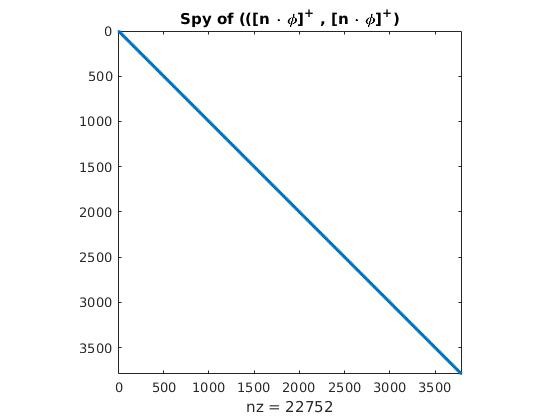
\includegraphics[width=\linewidth]{figure21.jpg}
    \label{fig:figure21}
	\caption{$((n \otimes \phi)^+,(n \otimes \phi)^+)_{\Gamma \cup \Gamma_D}$}      
  \end{subfigure}
  \begin{subfigure}{0.45\textwidth}
    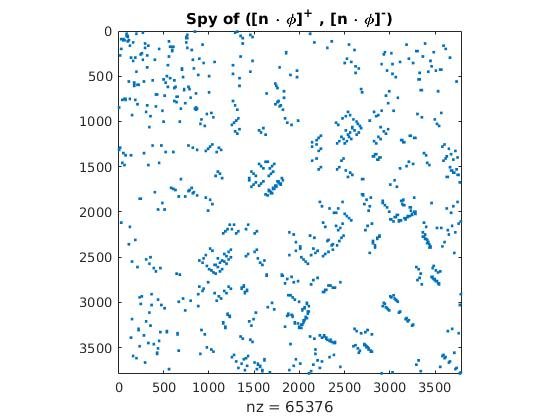
\includegraphics[width=\linewidth]{figure22.jpg}
    \label{fig:figure22}
	\caption{$((n \otimes \phi)^+,(n \otimes \phi)^-)_{\Gamma \cup \Gamma_D}$}      
  \end{subfigure}
\caption{Sparsity pattern of constituents of $([n \otimes \phi],[n \otimes \phi])_{\Gamma \cup \Gamma_D}$}
\label{figure_2_all}
\end{figure}

\end{frame}

%------------------------------------------------
\begin{frame}
\frametitle{Sparsity pattern}

\begin{figure}
    \begin{subfigure}{0.45\textwidth}
    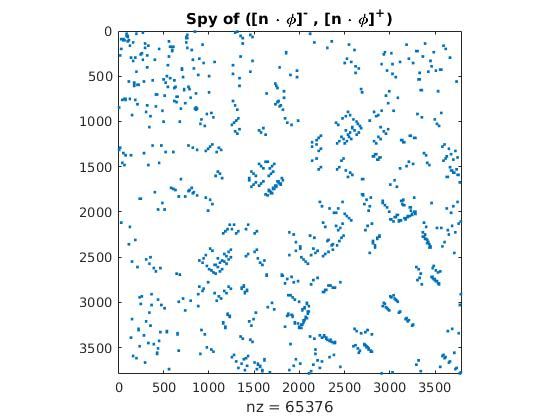
\includegraphics[width=\linewidth]{figure23.jpg}
    \label{fig:figure23}
	\caption{$((n \otimes \phi)^-,(n \otimes \phi)^+)_{\Gamma \cup \Gamma_D}$}      
  \end{subfigure}
    \begin{subfigure}{0.45\textwidth}
    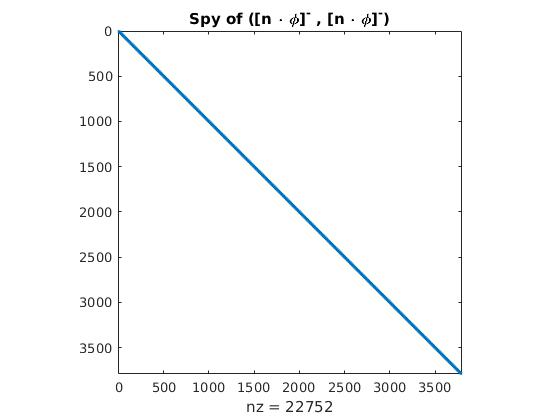
\includegraphics[width=\textwidth]{figure24.jpg}
    \label{fig:figure24}
	\caption{$((n \otimes \phi)^-,(n \otimes \phi)^-)_{\Gamma \cup \Gamma_D}$}      
  \end{subfigure}
\caption{Sparsity pattern of constituents of $([n \otimes \phi],[n \otimes \phi])_{\Gamma \cup \Gamma_D}$}
\label{figure_2_all}
\end{figure}

\end{frame}

%------------------------------------------------
\begin{frame}
\frametitle{Sparsity pattern}
\begin{figure}
  \begin{subfigure}{0.8\textwidth}	
\centering
  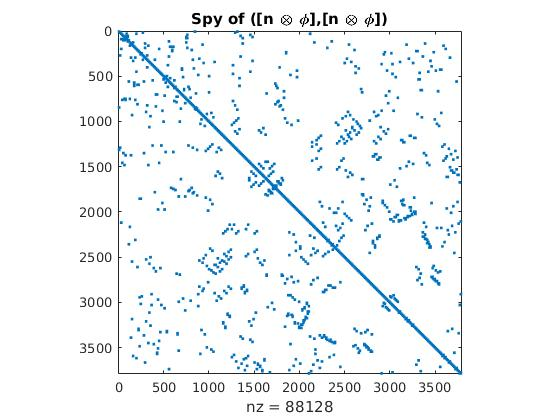
\includegraphics[width=0.8\textwidth]{figure2.jpg}
  \label{fig:figure2}
\end{subfigure}
\caption{Sparsity pattern of constituents of $([n \otimes \phi],[n \otimes \phi])_{\Gamma \cup \Gamma_D}$}
\label{figure_2_all}
\end{figure}
\end{frame}
%------------------------------------------------
\section{Numerical experiments}
%------------------------------------------------
\begin{frame}
\frametitle{Error definition}
\begin{itemize}
\item If $P_h$ is the computed solution and $P$ is the true solution, we define following errors:
\end{itemize}
\begin{block}{$L^2$ error}
\begin{equation}
P_{error,L^2} = (\int_{\Omega} |P - P_h|^2 )^\frac{1}{2} \mathrm{.}
\end{equation}
\end{block}
\begin{block}{$H_0$ error}
\begin{equation}
P_{error,H_0} = \sum_{k=1}^{nel} (\int_{\tau_k} |\nabla P - \nabla P_h|^2)^\frac{1}{2} \mathrm{.}
\end{equation}
\end{block}
\end{frame}
%------------------------------------------------
\begin{frame}
\frametitle{Stokes equation: Convergence test}
\begin{itemize}
\item Domain: unit square [0,1] $\times$ [0,1].
\item ${x=0}$ is dirichlet boundary with inflow velocity at point $(0,y)$ as $u = (y(1-y), 0)$.
\item The boundaries ${y = 0}$ and ${y = 1}$ are Dirichlet boundaries with no slip or zero velocity condition. The boundary ${x = 1}$ is a Neumann boundary with zero Neumann value i.e. $t = (0, 0)$. 
\item The source term is $f = (2 \nu - 1, 0)$.

\begin{block}{Analytical solution}
\begin{equation}
p = (1 - x) \textrm{,}
\end{equation}

\begin{equation} 
 u = (y(1-y), 0) \textrm{.}
\end{equation}
\end{block}
\end{itemize}
\end{frame}
%------------------------------------------------
\begin{frame}
\frametitle{Stokes equation: Convergence test}
\begin{figure}
\begin{subfigure}{\textwidth}	
  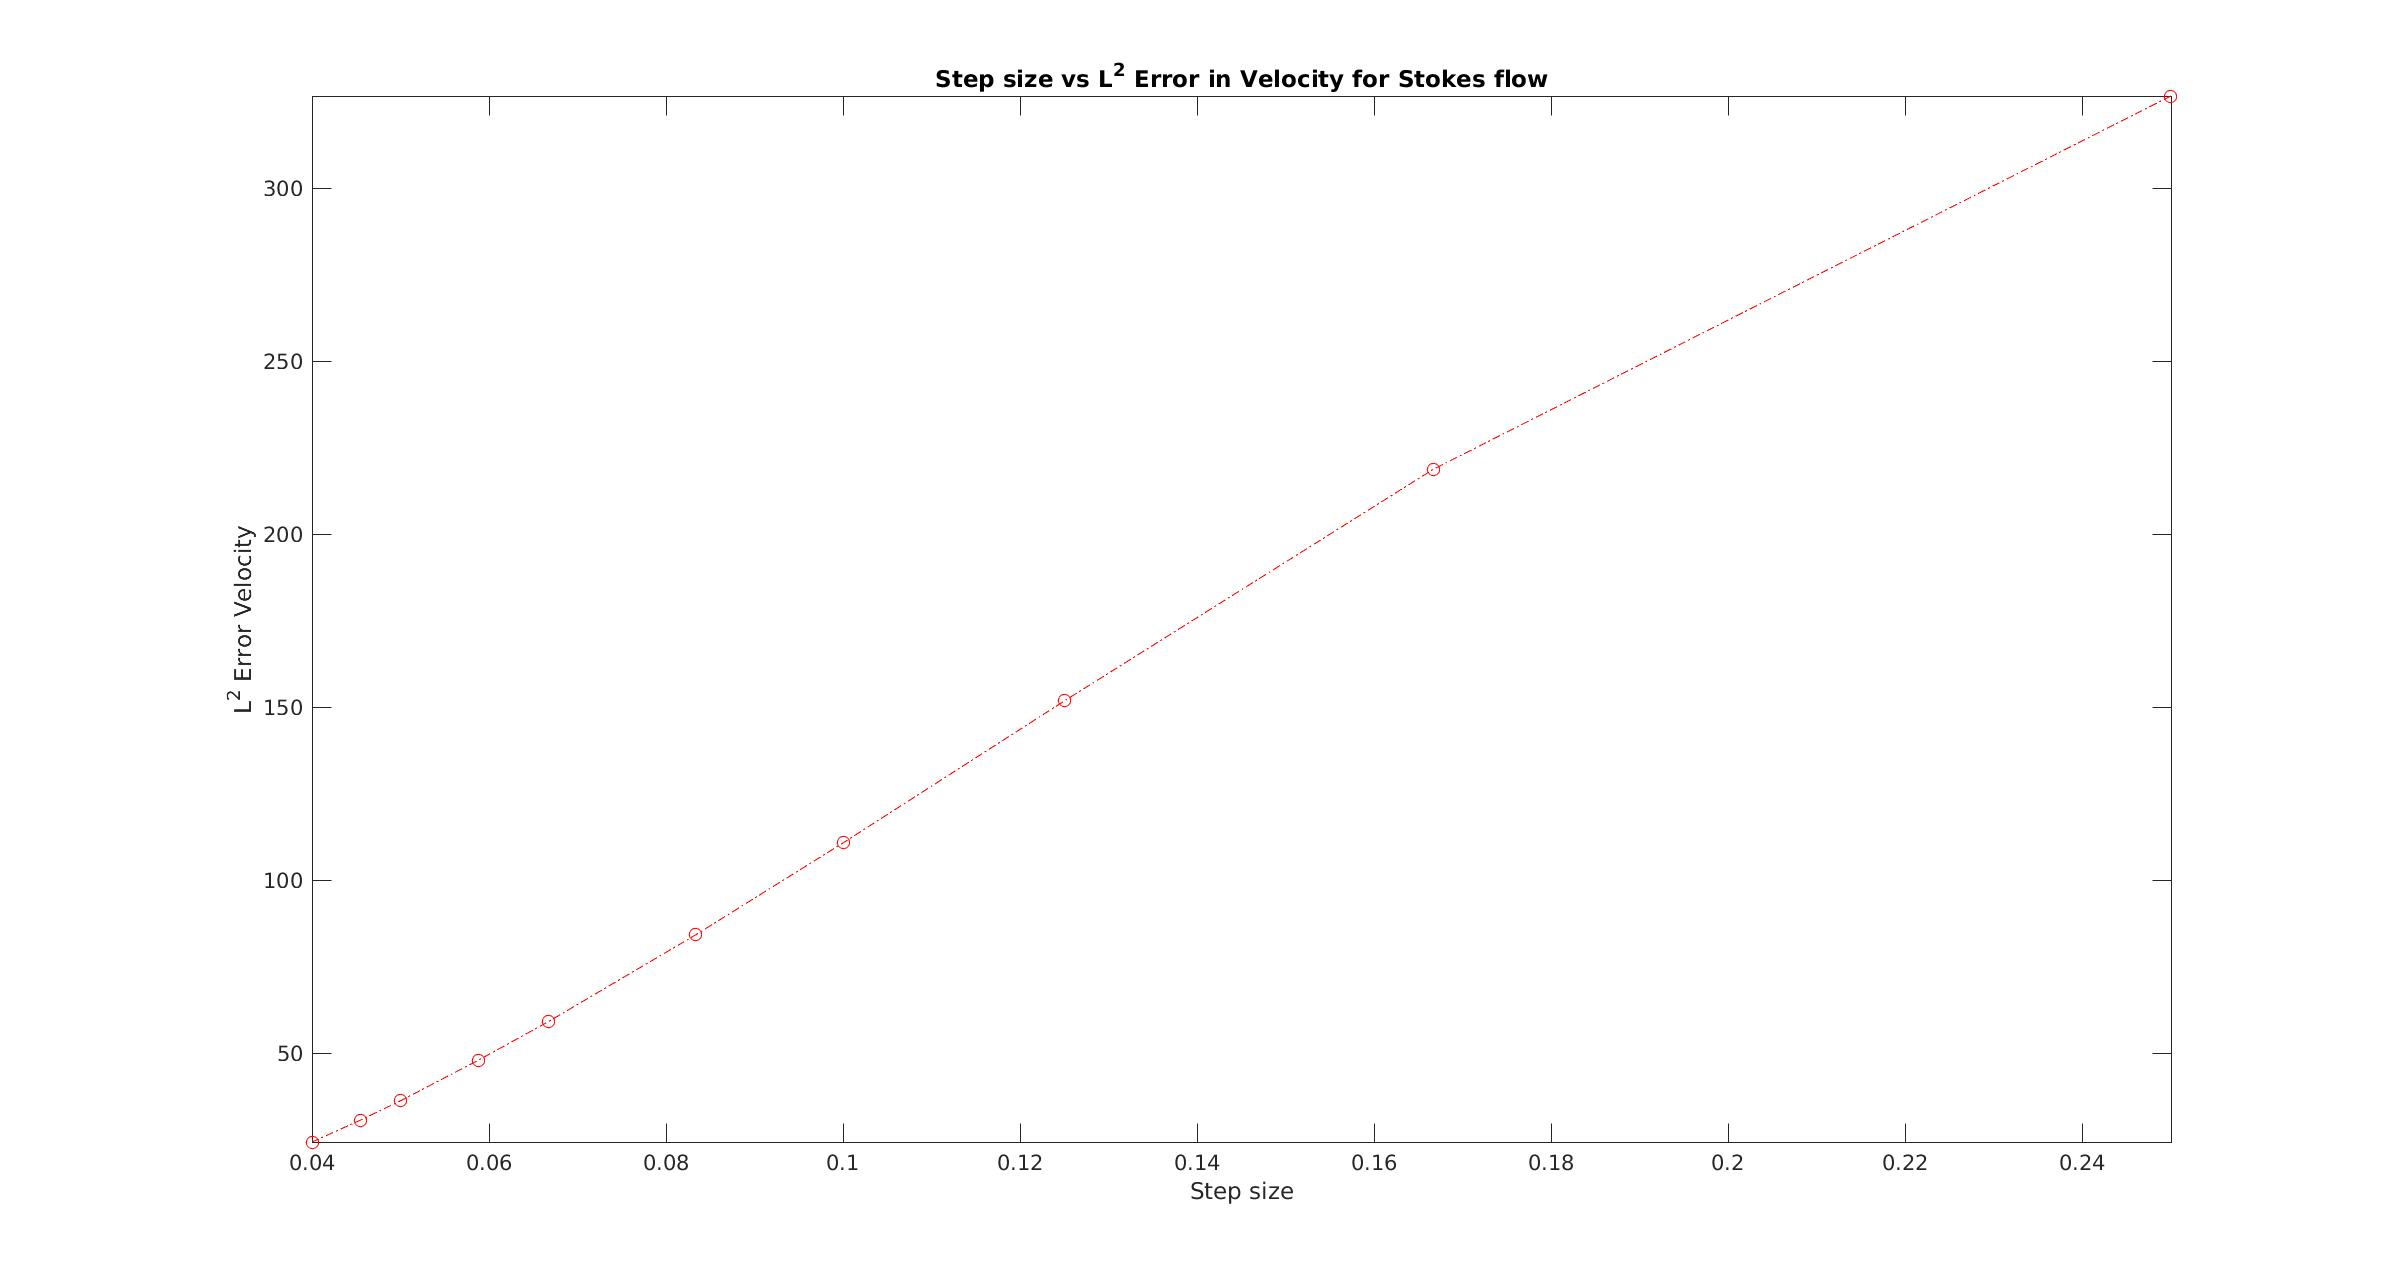
\includegraphics[width=\linewidth]{l2_velocity_stokes.jpg}
  \label{fig:vel_stoke_conv}
\end{subfigure}
\caption{$h-$convergence test for velocity in $L^2$ error}
\end{figure}
\end{frame}
%------------------------------------------------
%------------------------------------------------
\begin{frame}
\frametitle{Stokes equation: Convergence test}
\begin{figure}
\begin{subfigure}{\textwidth}	
  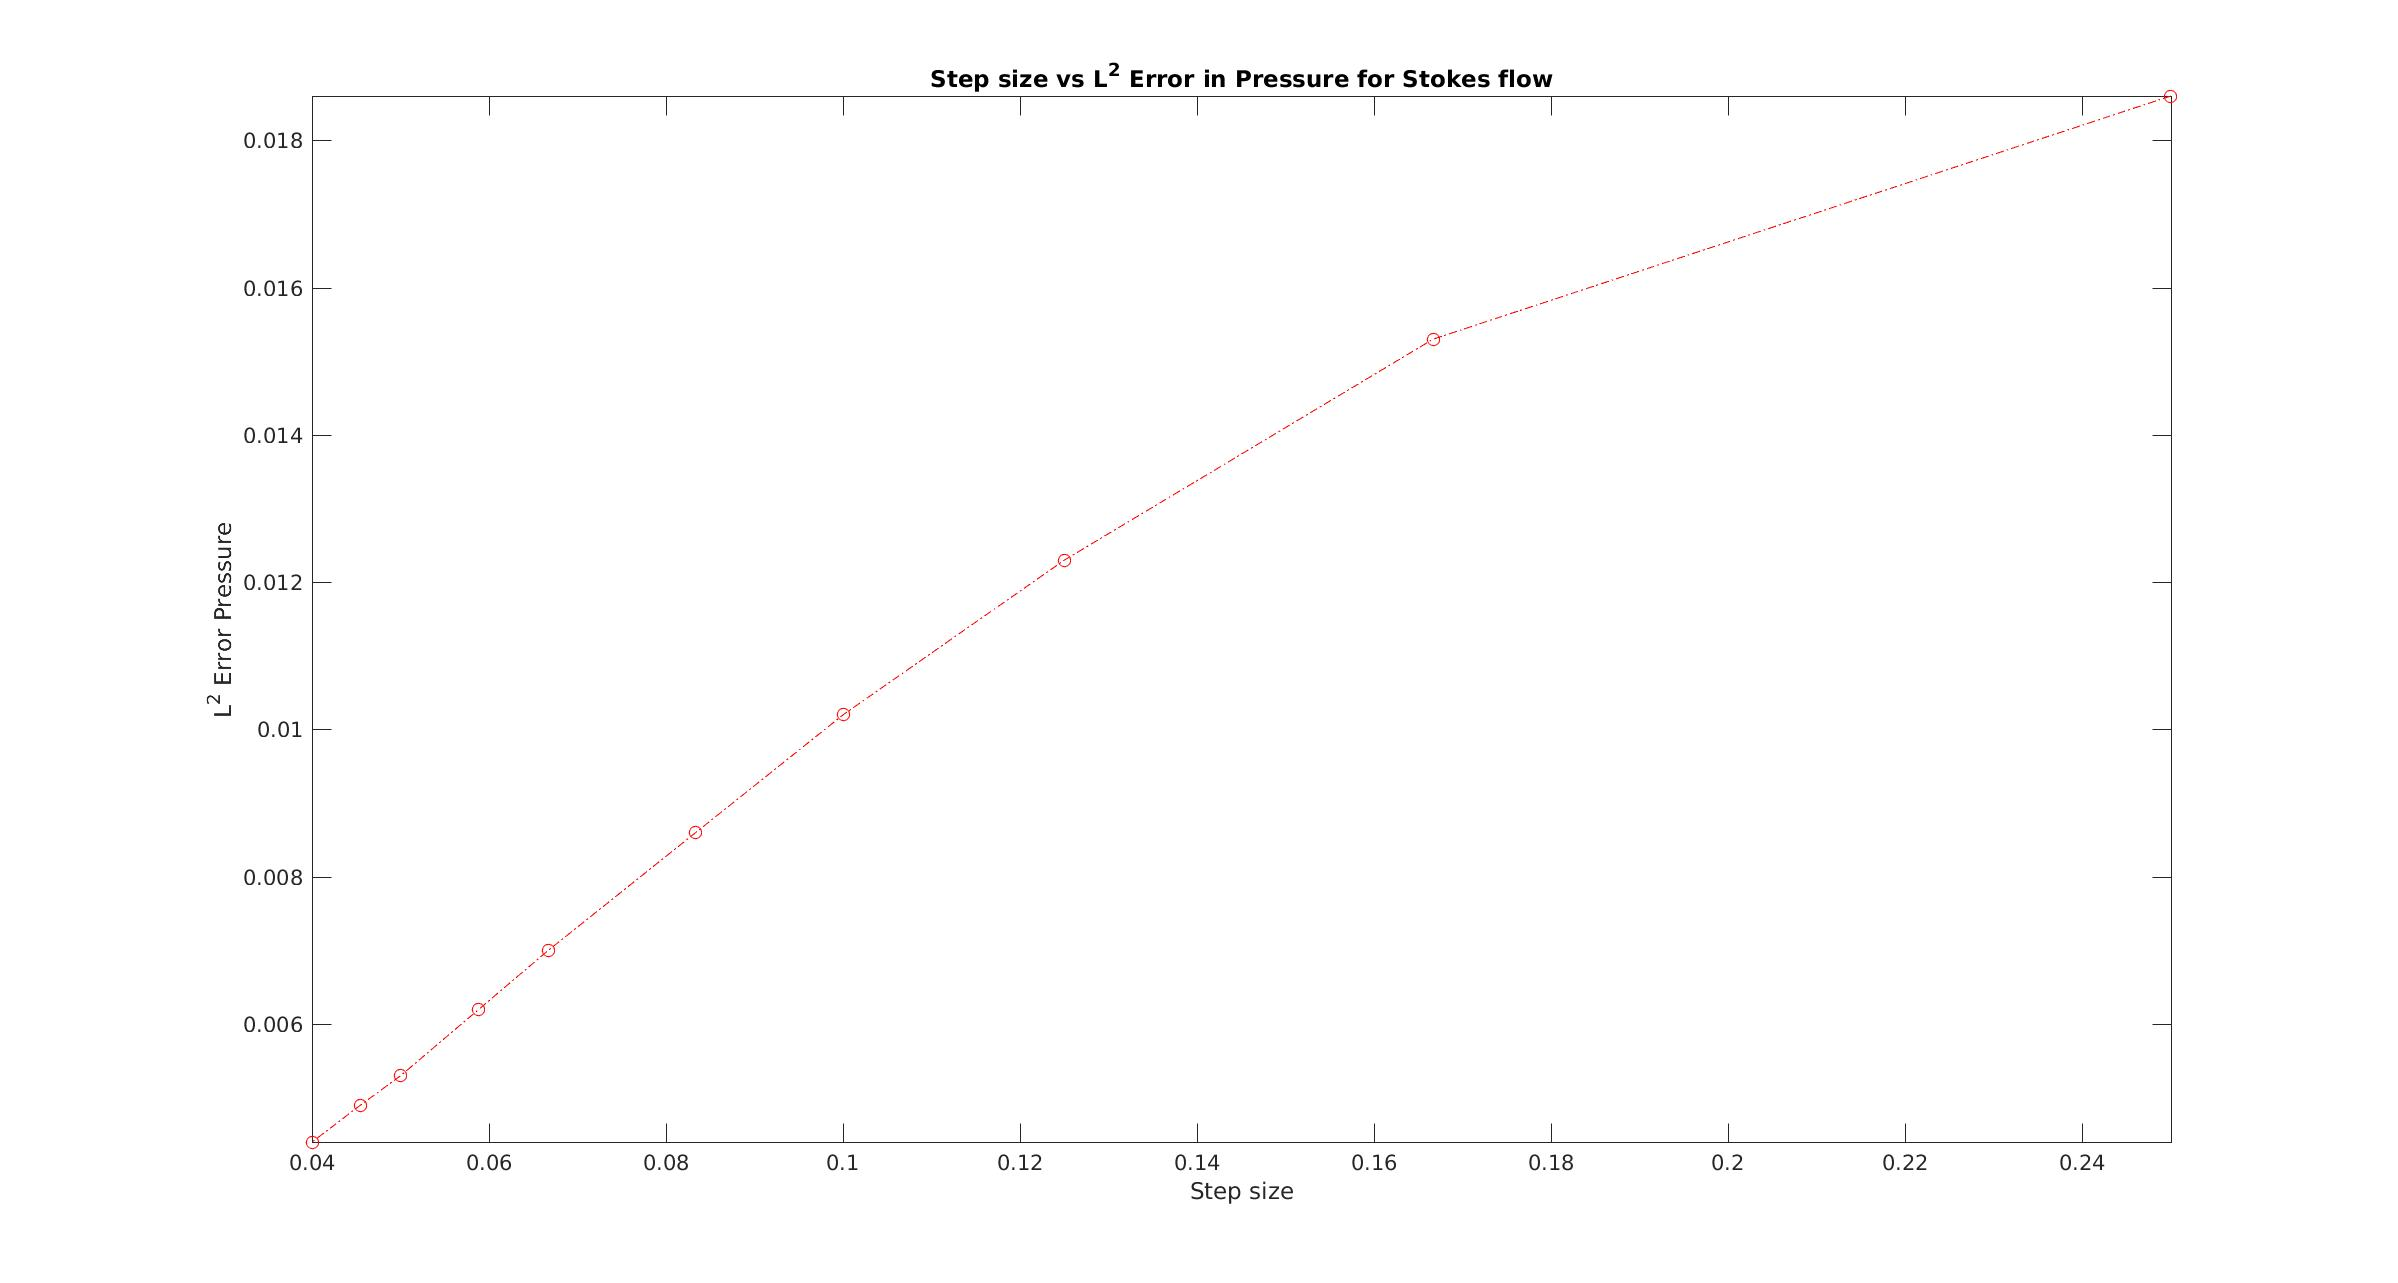
\includegraphics[width=\linewidth]{l2_pressure_stokes.jpg}
  \label{fig:pre_stoke_conv}
\end{subfigure}
\caption{$h-$convergence test for pressure in $L^2$ error}
\end{figure}
\end{frame}
%------------------------------------------------
\begin{frame}
\frametitle{Stokes equation: Convergence test}
\begin{figure}
\begin{subfigure}{\textwidth}	
  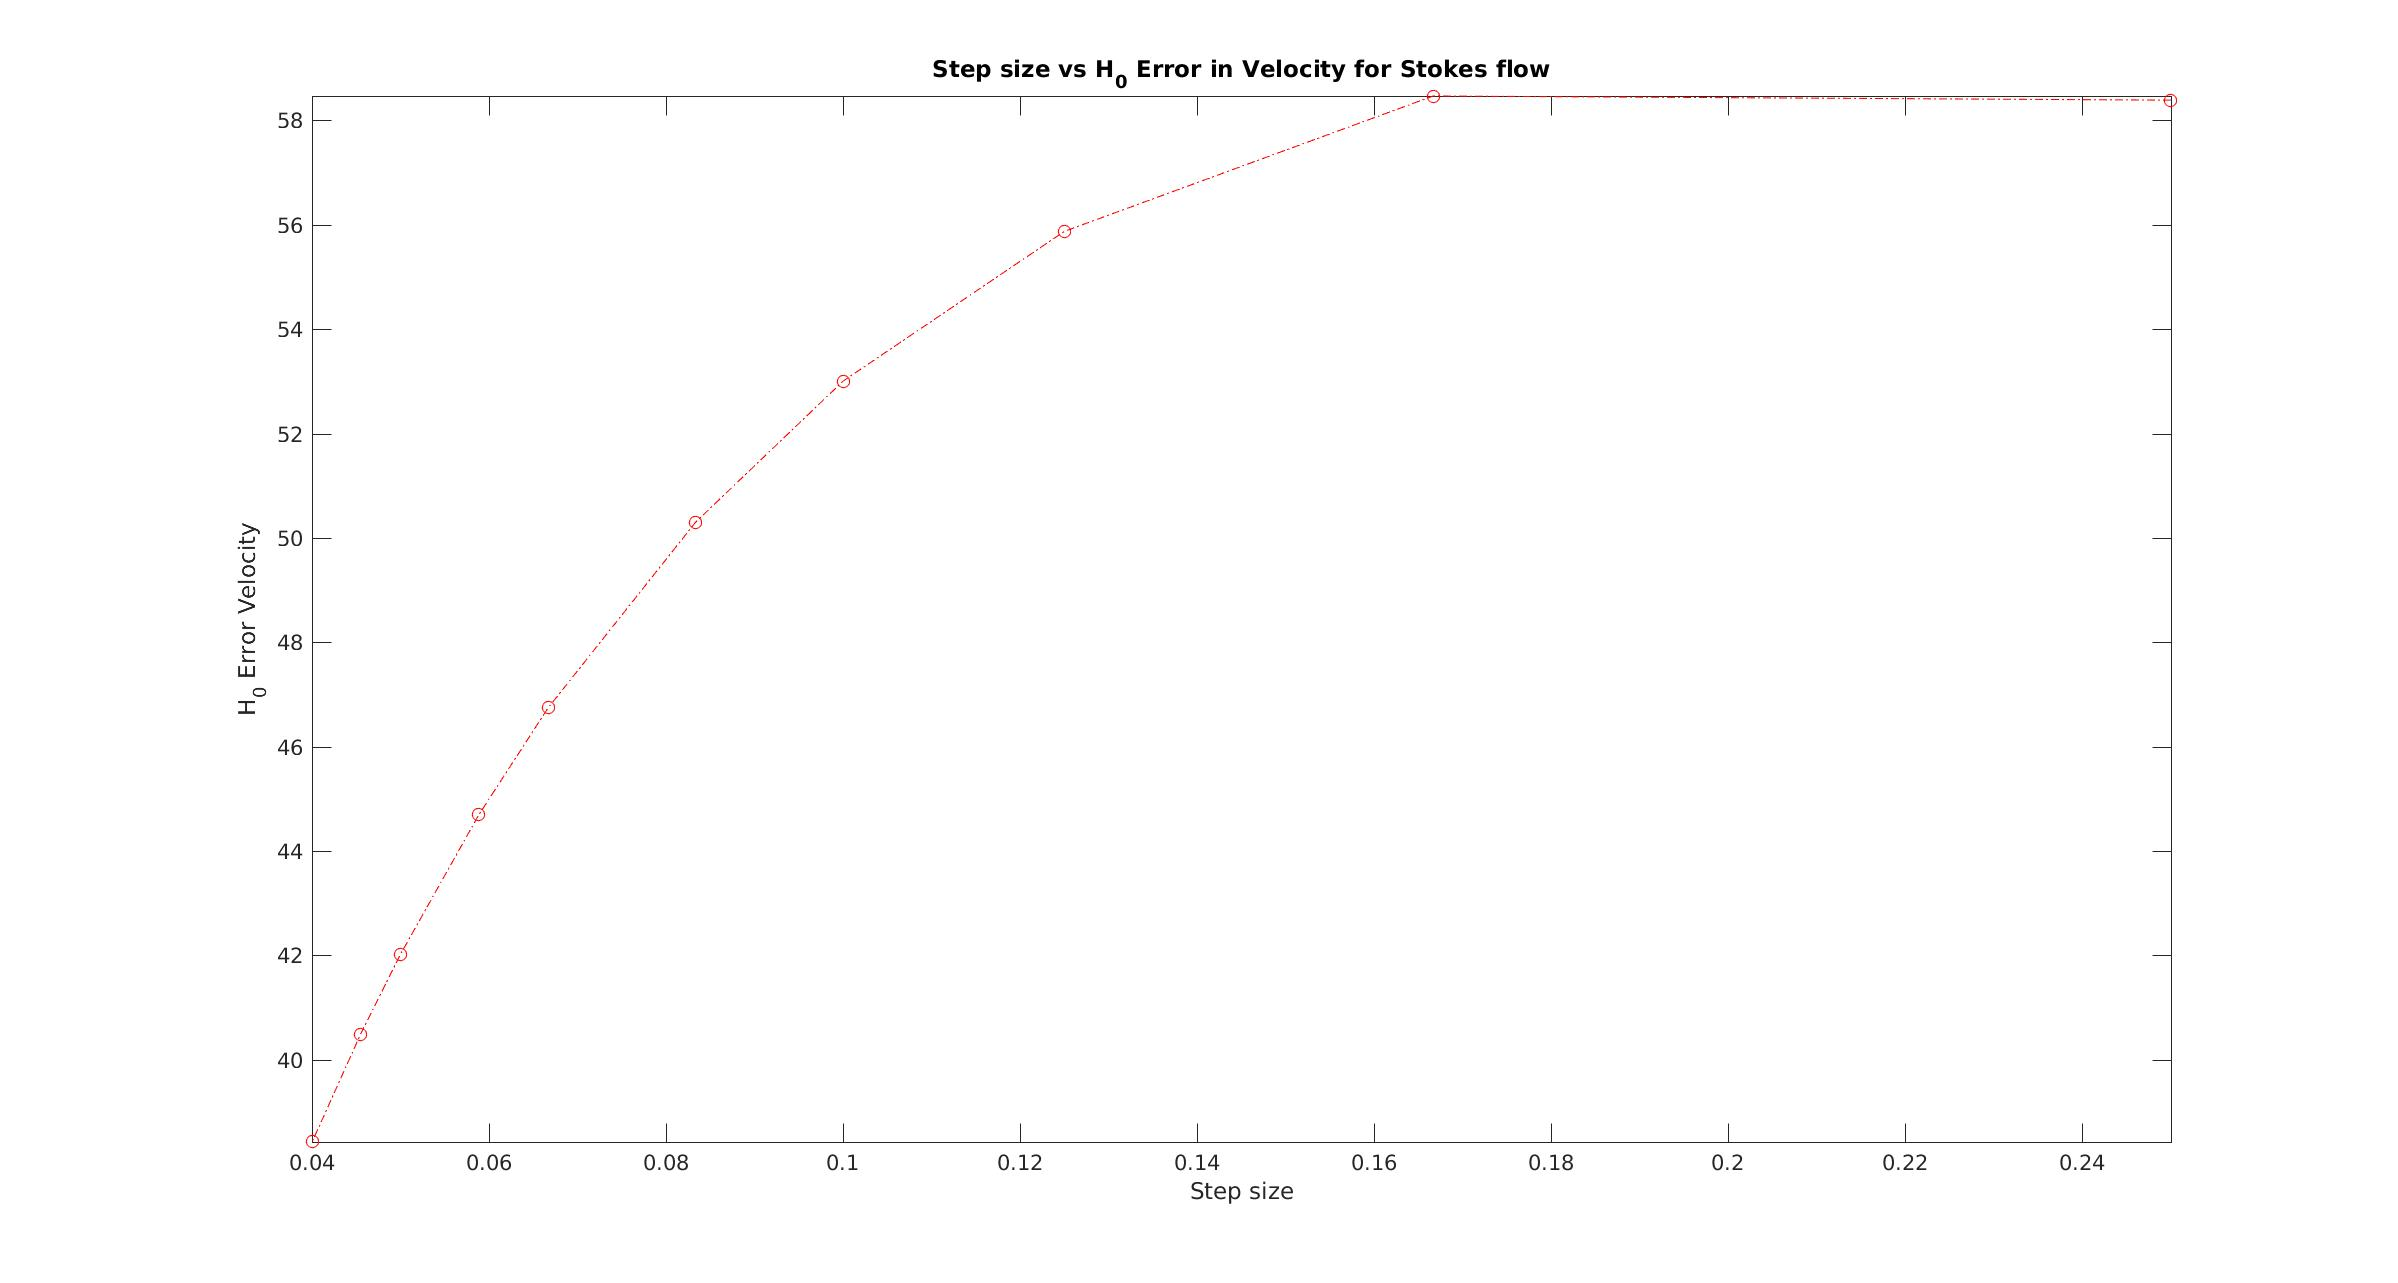
\includegraphics[width=\linewidth]{h0_velocity_stokes.jpg}
  \label{fig:vel_stoke_conv_h0}
\end{subfigure}
\caption{$h-$convergence test for velocity in $H_0$ error }
\end{figure}
\end{frame}
%------------------------------------------------
\begin{frame}
\frametitle{Stokes equation: Convergence test}
\begin{figure}
\begin{subfigure}{\textwidth}	
  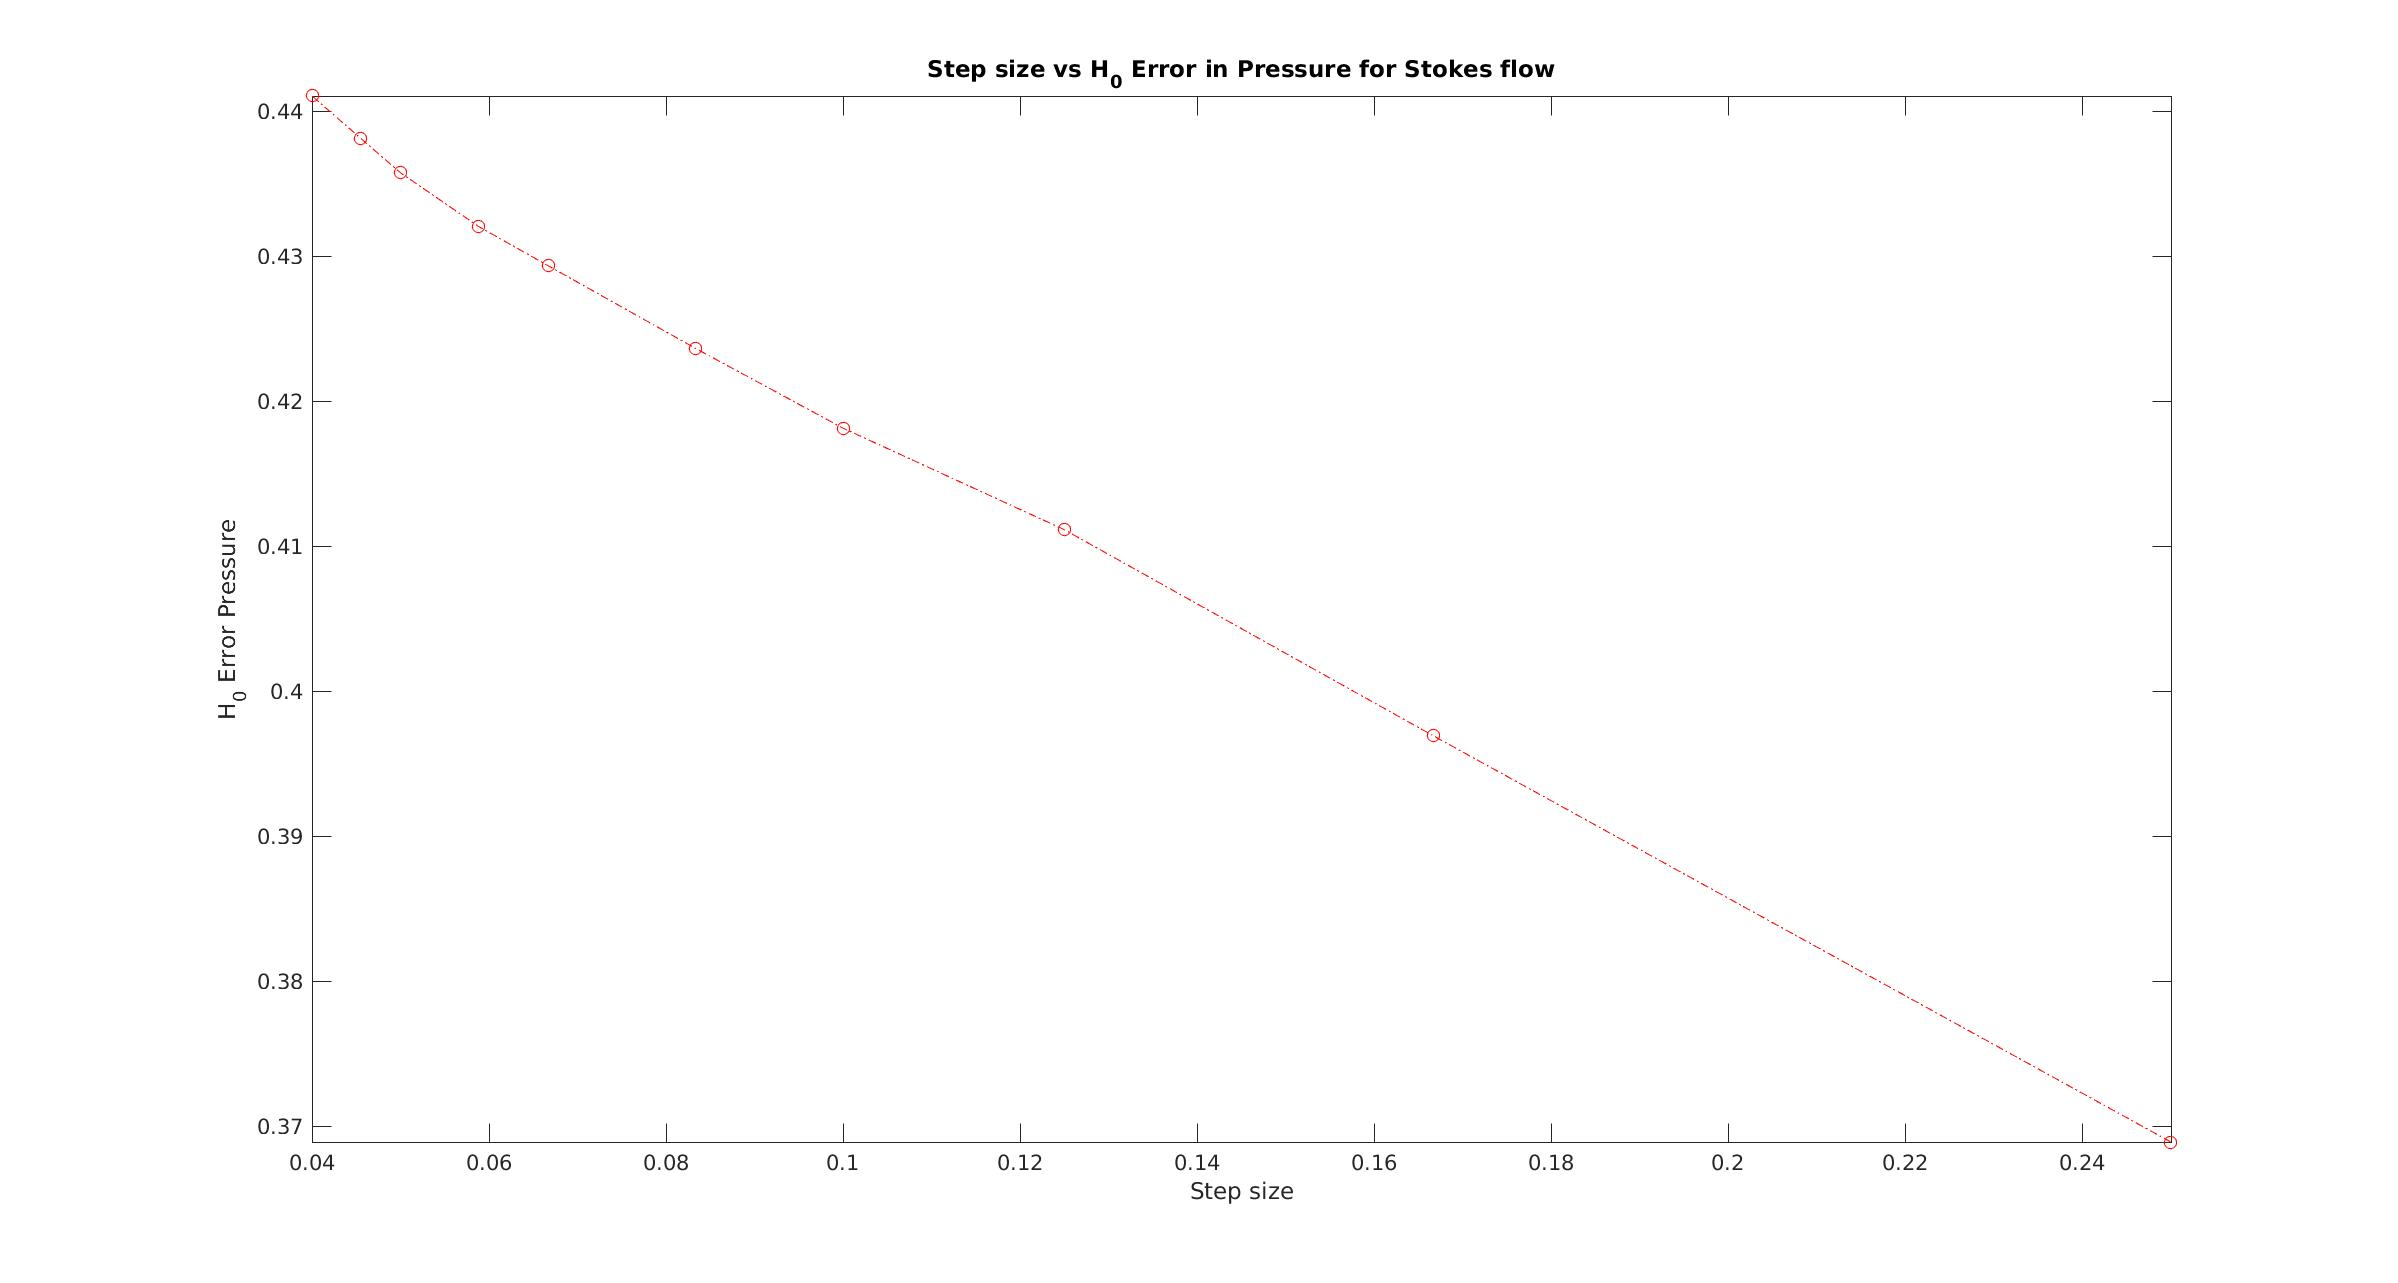
\includegraphics[width=\linewidth]{h0_pressure_stokes.jpg}
  \label{fig:pre_stoke_conv_h0}
\end{subfigure}
\caption{$h-$convergence test for pressure in $H_0$ error}
\end{figure}
\end{frame}
%------------------------------------------------
\begin{frame}
\frametitle{Stokes equation: Convergence test}
\begin{figure}
\begin{subfigure}{0.9\textwidth}
\centering
  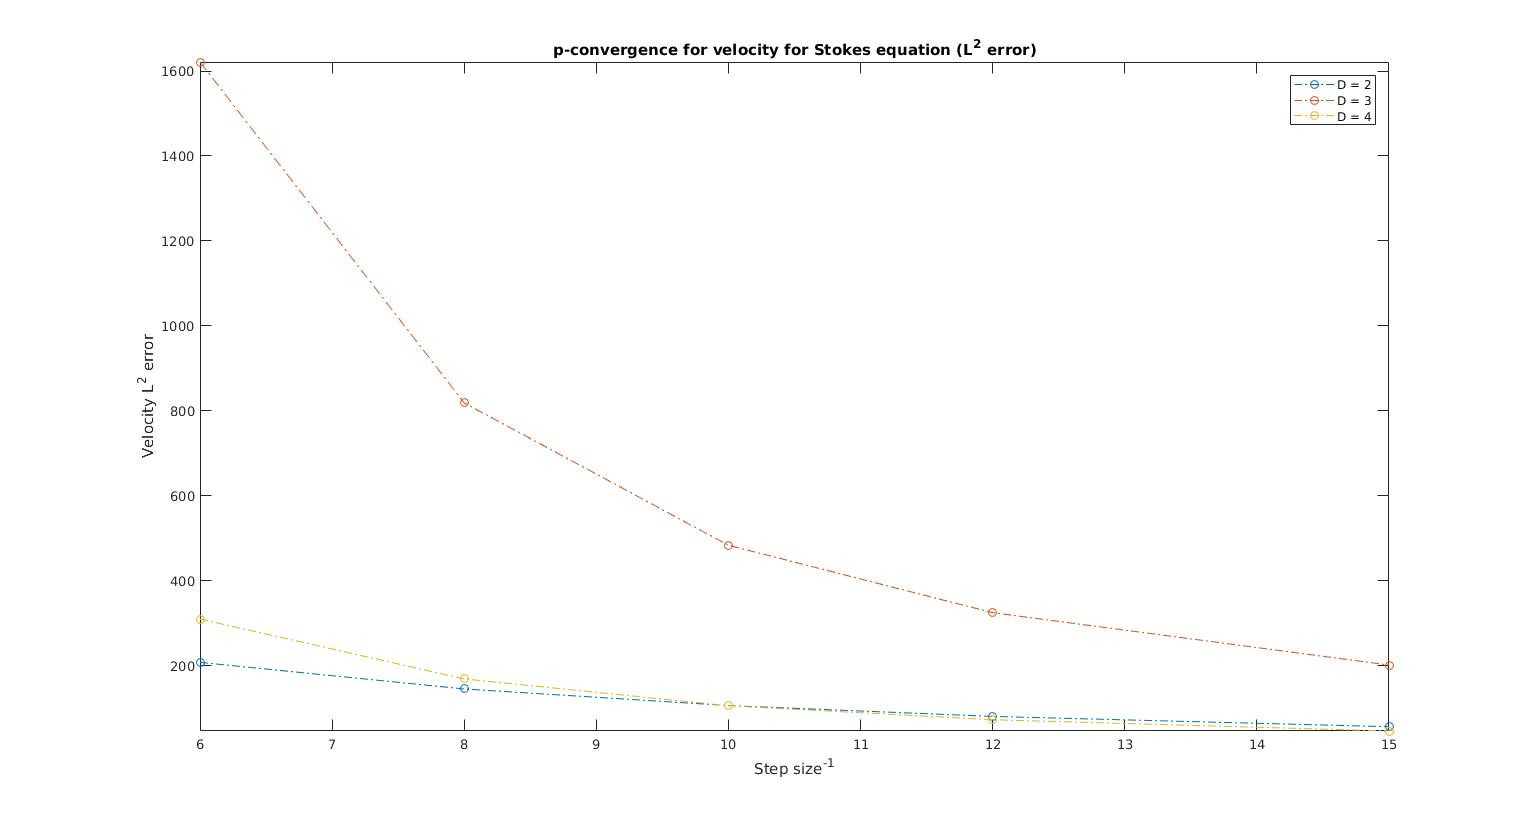
\includegraphics[width=0.9\linewidth]{p_conv_velocity_l2_stokes.jpg}
  \label{p_convergence_velocity_l2}
  \caption{$p-$convergence for velocity in $L^2$ error}
\end{subfigure}
\end{figure}
\end{frame}
%------------------------------------------------
\begin{frame}
\frametitle{Stokes equation: Convergence test}
\begin{figure}
\begin{subfigure}{0.9\textwidth}
\centering
  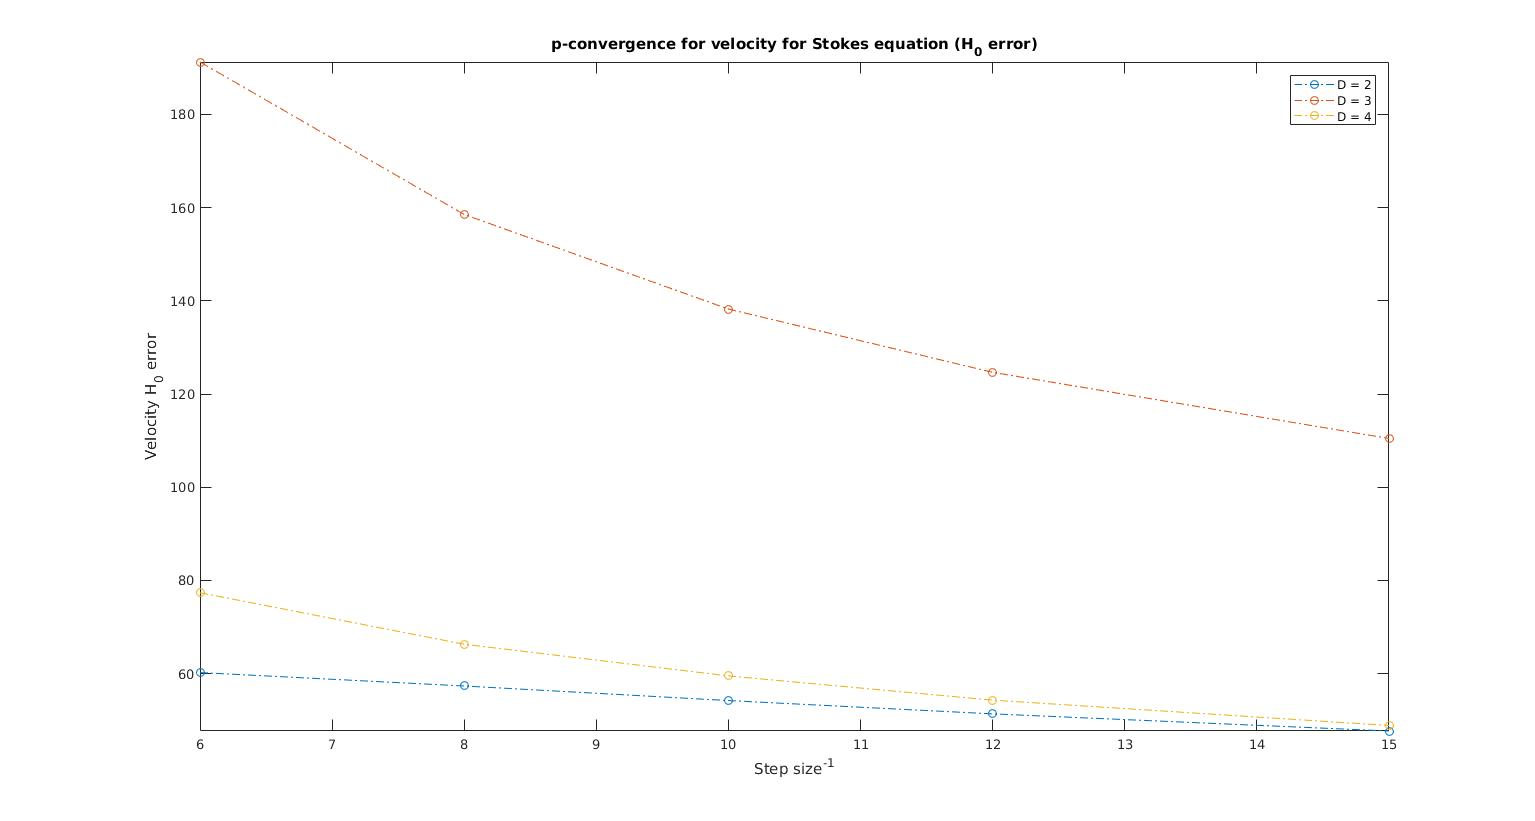
\includegraphics[width=0.9\linewidth]{p_conv_velocity_h0_stokes.jpg}
  \label{p_convergence_velocity_h0}
\caption{$p-$convergence for velocity in $H_0$ error}
\end{subfigure}
\end{figure}
\end{frame}
%------------------------------------------------
\begin{frame}
\frametitle{Stokes equation: Convergence test}
\begin{figure}
\begin{subfigure}{0.9\textwidth}
\centering
  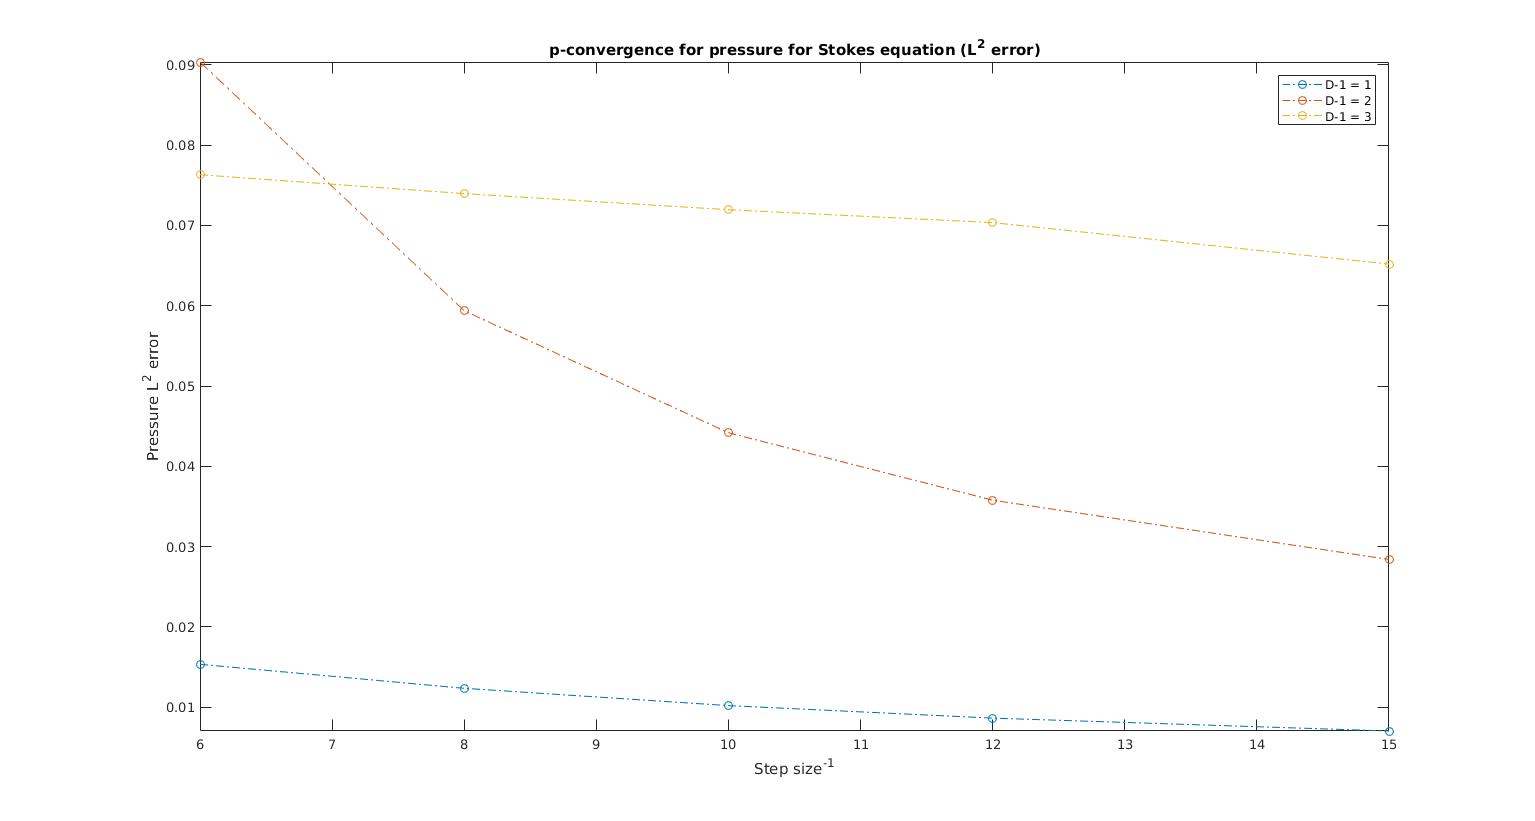
\includegraphics[width=0.9\linewidth]{p_conv_pressure_l2_stokes.jpg}
  \label{p_convergence_pressure_l2}
\end{subfigure}
\caption{$p-$convergence for pressure in $L^2$ error}
\label{p_conv_stokes_flow}
\end{figure}
\end{frame}
%------------------------------------------------
\begin{frame}
\frametitle{Stokes equation: Flow around cylinder}
\begin{itemize}
\item Domain: [0,1] $\times$ [0,1] with a cut out cylinder of diameter 0.2 centered at $(0.5,0.5)$.
\item The boundary ${x=0}$ is Dirichlet boundary with inflow velocity at point $(0,y)$ as $u = (y(1-y), 0)$. 
\item The boundaries ${y = 0}$ and ${y = 1}$ are Dirichlet boundaries with no slip or zero velocity condition. The boundary ${x = 1}$ is a Neumann boundary with zero Neumann value i.e. $t = (0, 0)$. 
\item The source term is $f = (0, 0)$.
\end{itemize}
\end{frame}
%------------------------------------------------
\begin{frame}
\frametitle{Stokes equation: Flow around cylinder}
\begin{figure}
\begin{subfigure}{0.3\textwidth}	
    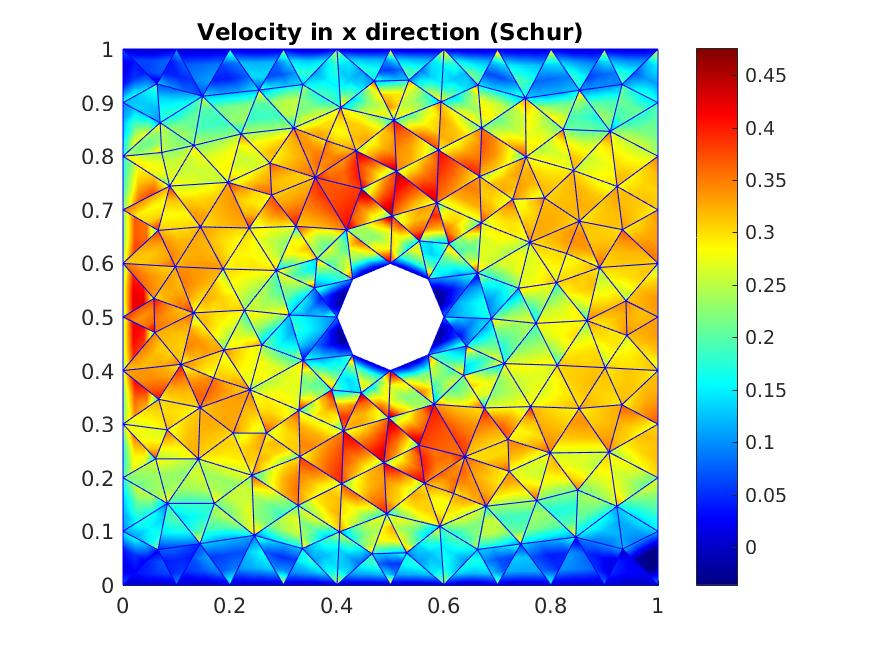
\includegraphics[width=\linewidth]{cylinder_schur_vx.jpg}
    \caption{$x-$velocity}
    \label{x_vel_stoke_schur}
\end{subfigure}
\begin{subfigure}{0.3\textwidth}	
    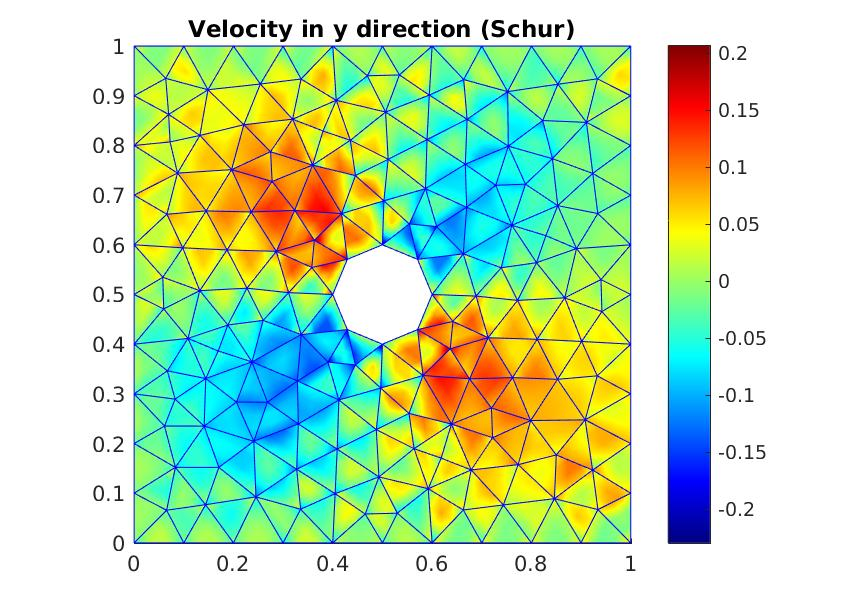
\includegraphics[width=\linewidth]{cylinder_schur_vy.jpg}
    \caption{$y-$velocity}
     \label{y_vel_stoke_schur}
\end{subfigure}
\begin{subfigure}{0.3\textwidth}	
    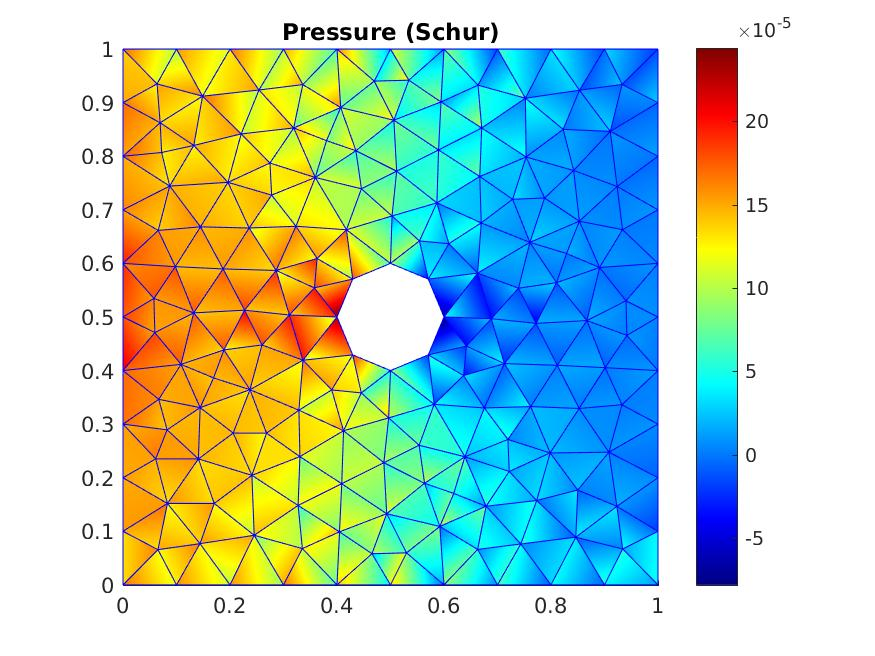
\includegraphics[width=\linewidth]{cylinder_schur_pressure.jpg}
    \caption{Pressure}
      \label{pressure_stoke_schur}
\end{subfigure}
\caption{Flow over cylinder}
\label{flow_over_cylinder_schur}
\end{figure}

\end{frame}
%------------------------------------------------
\begin{frame}
\frametitle{Stokes equation: Lid driven cavity}
\begin{itemize}
\item Domain: unit square [0,1] $\times$ [0,1].
\item Boundaries ${x = 0}, {x = 1}$ and ${y = 0}$, we impose no slip or zero velocity Dirichlet condition. 
\item On ${y = 1}$, we impose Dirichlet condition with Dirichlet velocity,
\begin{equation}
\begin{split}
u = (10x,0) \quad \textrm{for} \quad 0 \leq x \leq 0.1 \textrm{,}\\
u = (1,0) \quad \textrm{for} \quad 0.1 \leq x \leq 0.9 \textrm{,}\\
u = (10 - 10x,0) \quad \textrm{for} \quad 0.9 \leq x \leq 1 \textrm{.}
\end{split}
\end{equation}
\end{itemize}
\end{frame}
%------------------------------------------------
\begin{frame}
\frametitle{Stokes equation: Lid driven cavity}
\begin{figure}
\begin{subfigure}{0.3\textwidth}	
  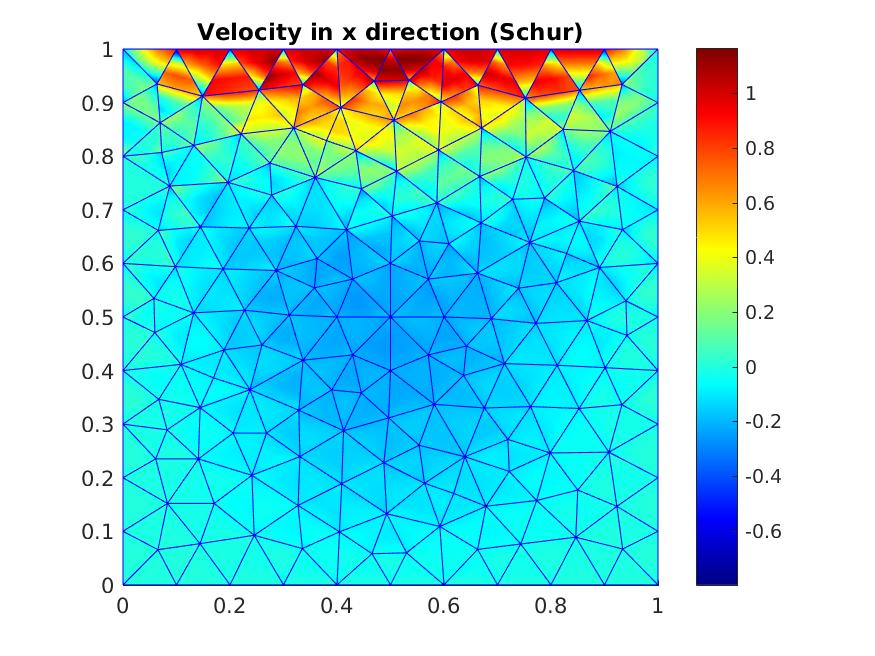
\includegraphics[width=\linewidth]{lid_schur_vx.jpg}
  \caption{$x-$velocity} 
  \label{x_vel_stoke_schur_lid}
\end{subfigure}
\begin{subfigure}{0.3\textwidth}	
  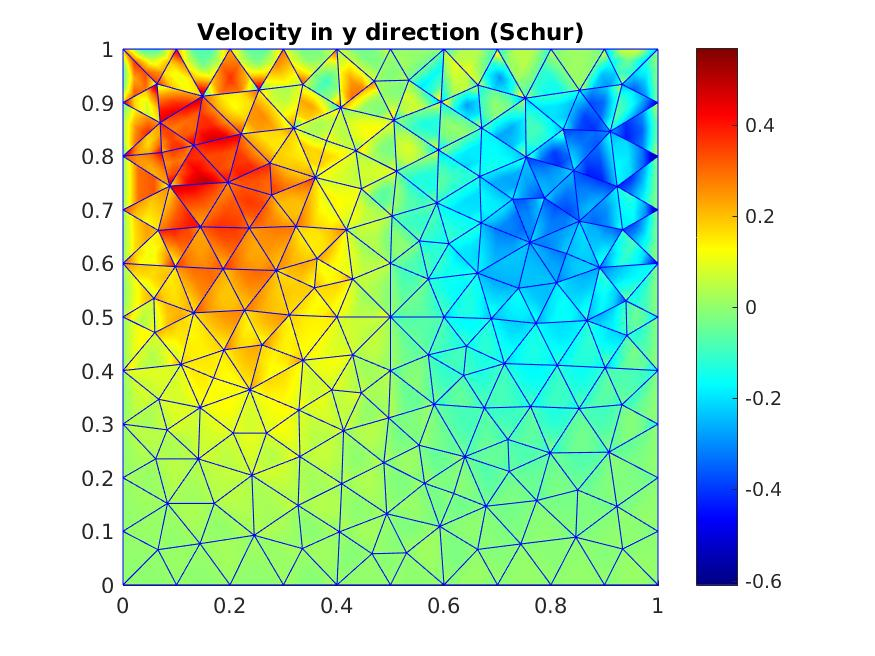
\includegraphics[width=\linewidth]{lid_schur_vy.jpg}
    \caption{$y-$velocity} 
    \label{y_vel_stoke_schur_lid}
\end{subfigure}
\begin{subfigure}{0.3\textwidth}	
  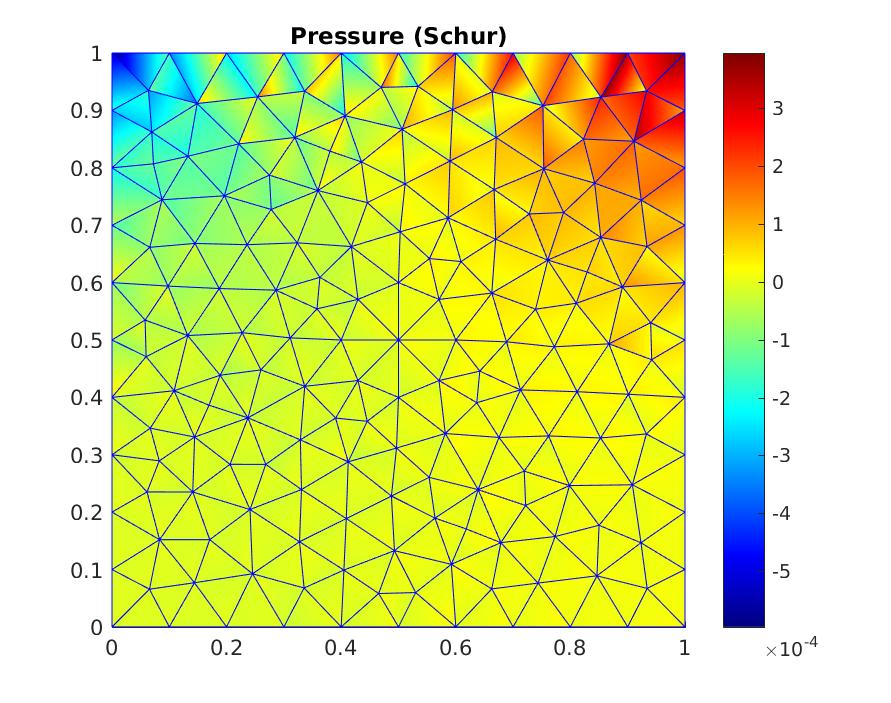
\includegraphics[width=\linewidth]{lid_schur_pressure.jpg}
    \caption{Pressure} 
    \label{pressure_stoke_schur_lid}
\end{subfigure}
\caption{Lid driven cavity problem (Schur complement method)}
\label{stoke_schur_lid}
\end{figure}
\end{frame}
%------------------------------------------------
\begin{frame}
\frametitle{Stokes equation: Lid driven cavity}
\begin{figure}
\begin{subfigure}{0.3\textwidth}	
  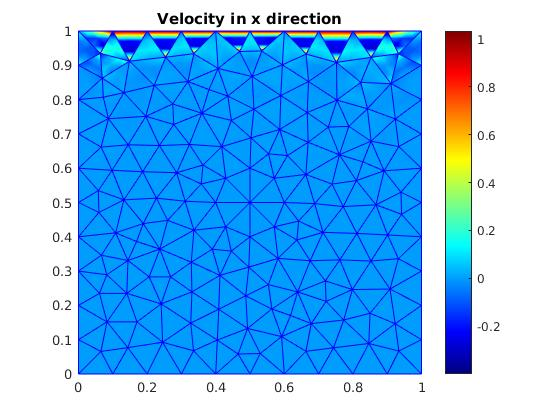
\includegraphics[width=\linewidth]{lid_bicgstab_vx.jpg}
  \caption{$x-$velocity} 
  \label{x_vel_stoke_bicgstab_lid}
\end{subfigure}
\begin{subfigure}{0.3\textwidth}	
  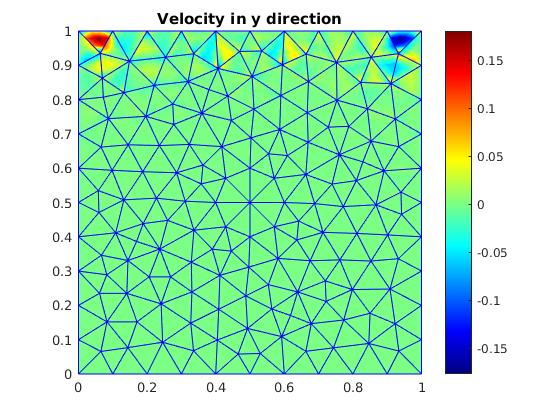
\includegraphics[width=\linewidth]{lid_bicgstab_vy.jpg}
  \caption{$y-$velocity} 
  \label{y_vel_stoke_bicgstab_lid}
\end{subfigure}
\begin{subfigure}{0.3\textwidth}	
  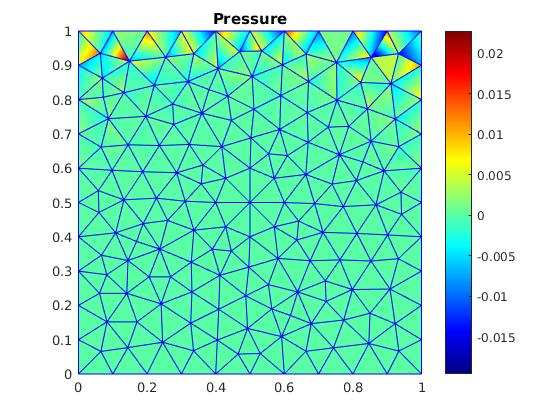
\includegraphics[width=\linewidth]{lid_bicgstab_pressure.jpg}
  \caption{Pressure} 
  \label{pressure_stoke_bicgstab_lid}
\end{subfigure}
\caption{Lid driven cavity problem ($bicgstab$ solver)}
\label{stoke_bicgstab_lid}
\end{figure}
\end{frame}
%------------------------------------------------
\begin{frame}
\frametitle{Penalty parameter}
\begin{figure}
\begin{subfigure}{0.25\textwidth}	
  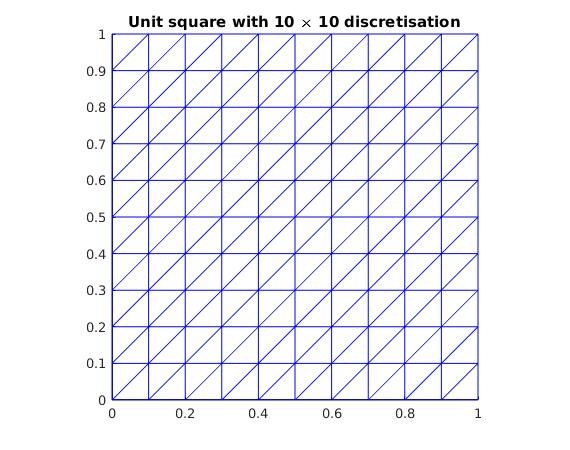
\includegraphics[width=\linewidth]{grid_penalty_parameter.jpg}
  \label{grid_penalty_para}
\end{subfigure}
\begin{subfigure}{0.7\textwidth}	
	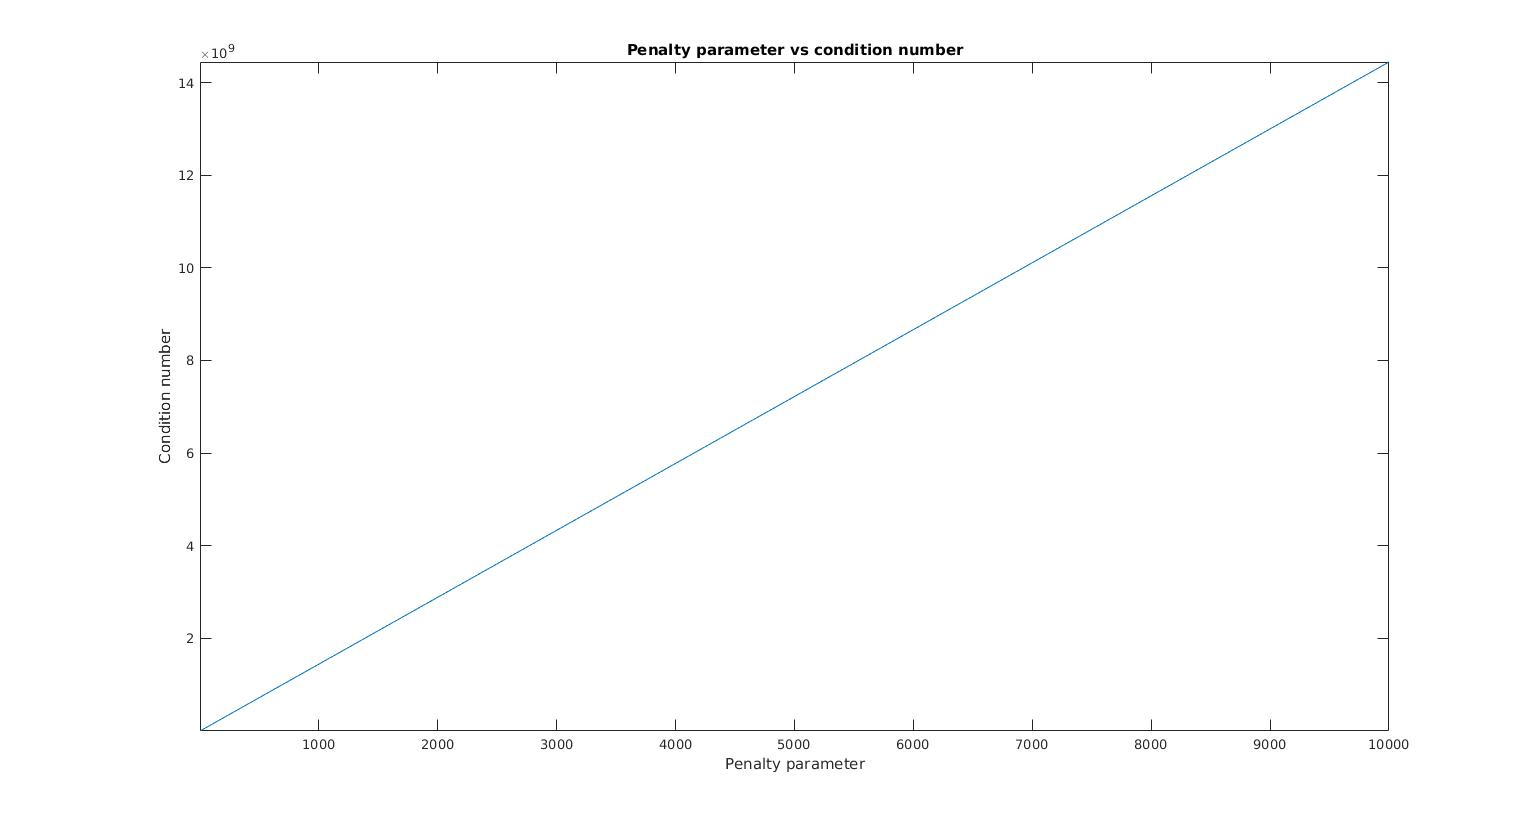
\includegraphics[width=\linewidth]{penalty_condition_number.jpg}
	\label{penalty_condition_number}
\end{subfigure}
\caption{Effect of penalty parameter}
\label{effect_penalty_parameter}
\end{figure}
\end{frame}
%------------------------------------------------
\begin{frame}
\frametitle{Solver performance}

Relative residual is measured as $\frac{||B-AX||_2}{||B||_2}$ for equation $AX=B$.

\begin{longtable}{| p{.25\textwidth} | p{.25\textwidth} | p{.25\textwidth} |}
\hline
\textbf{Solver/Method} & \textbf{Relative residual} & \textbf{Run time}\\
\hline
Schur complement method & 2.4436e-08 & 6.6253 Seconds\\
\hline
$minres$ & 2.4618e-05 & 35.7372 Seconds\\
\hline
$bicgstab$ & 9.0071e-05 & 58.3472 Seconds\\
\hline
\end{longtable}

\end{frame}
%------------------------------------------------
\begin{frame}
\frametitle{Navier-Stokes equation: Convergence test}
\begin{itemize}
\item Domain: unit square [0,1] $\times$ [0,1].
\item ${x=0}$ is dirichlet boundary with inflow velocity at point $(0,y)$ as $u = a*(y(1-y), 0)$.
\item The boundary ${x = 1}$ is a Neumann boundary with zero Neumann value i.e. $t = (0, 0)$. 
\item Specified source term
\end{itemize}
\begin{block}{Analytical solution}
\begin{equation}
p = x(1 - x) \textrm{,}
\end{equation}
\begin{equation} 
\begin{split}
u = (x^2(1-y)^2(2y-6y^2+4y^3),\\-y^2(1-y)^2(2x-6x^2+4x^3)) \textrm{.}
\end{split}
\end{equation}
\end{block}
\end{frame}
%------------------------------------------------
\begin{frame}
\frametitle{Navier-Stokes equation: Convergence test}
\begin{figure}
\begin{subfigure}{\textwidth}	
    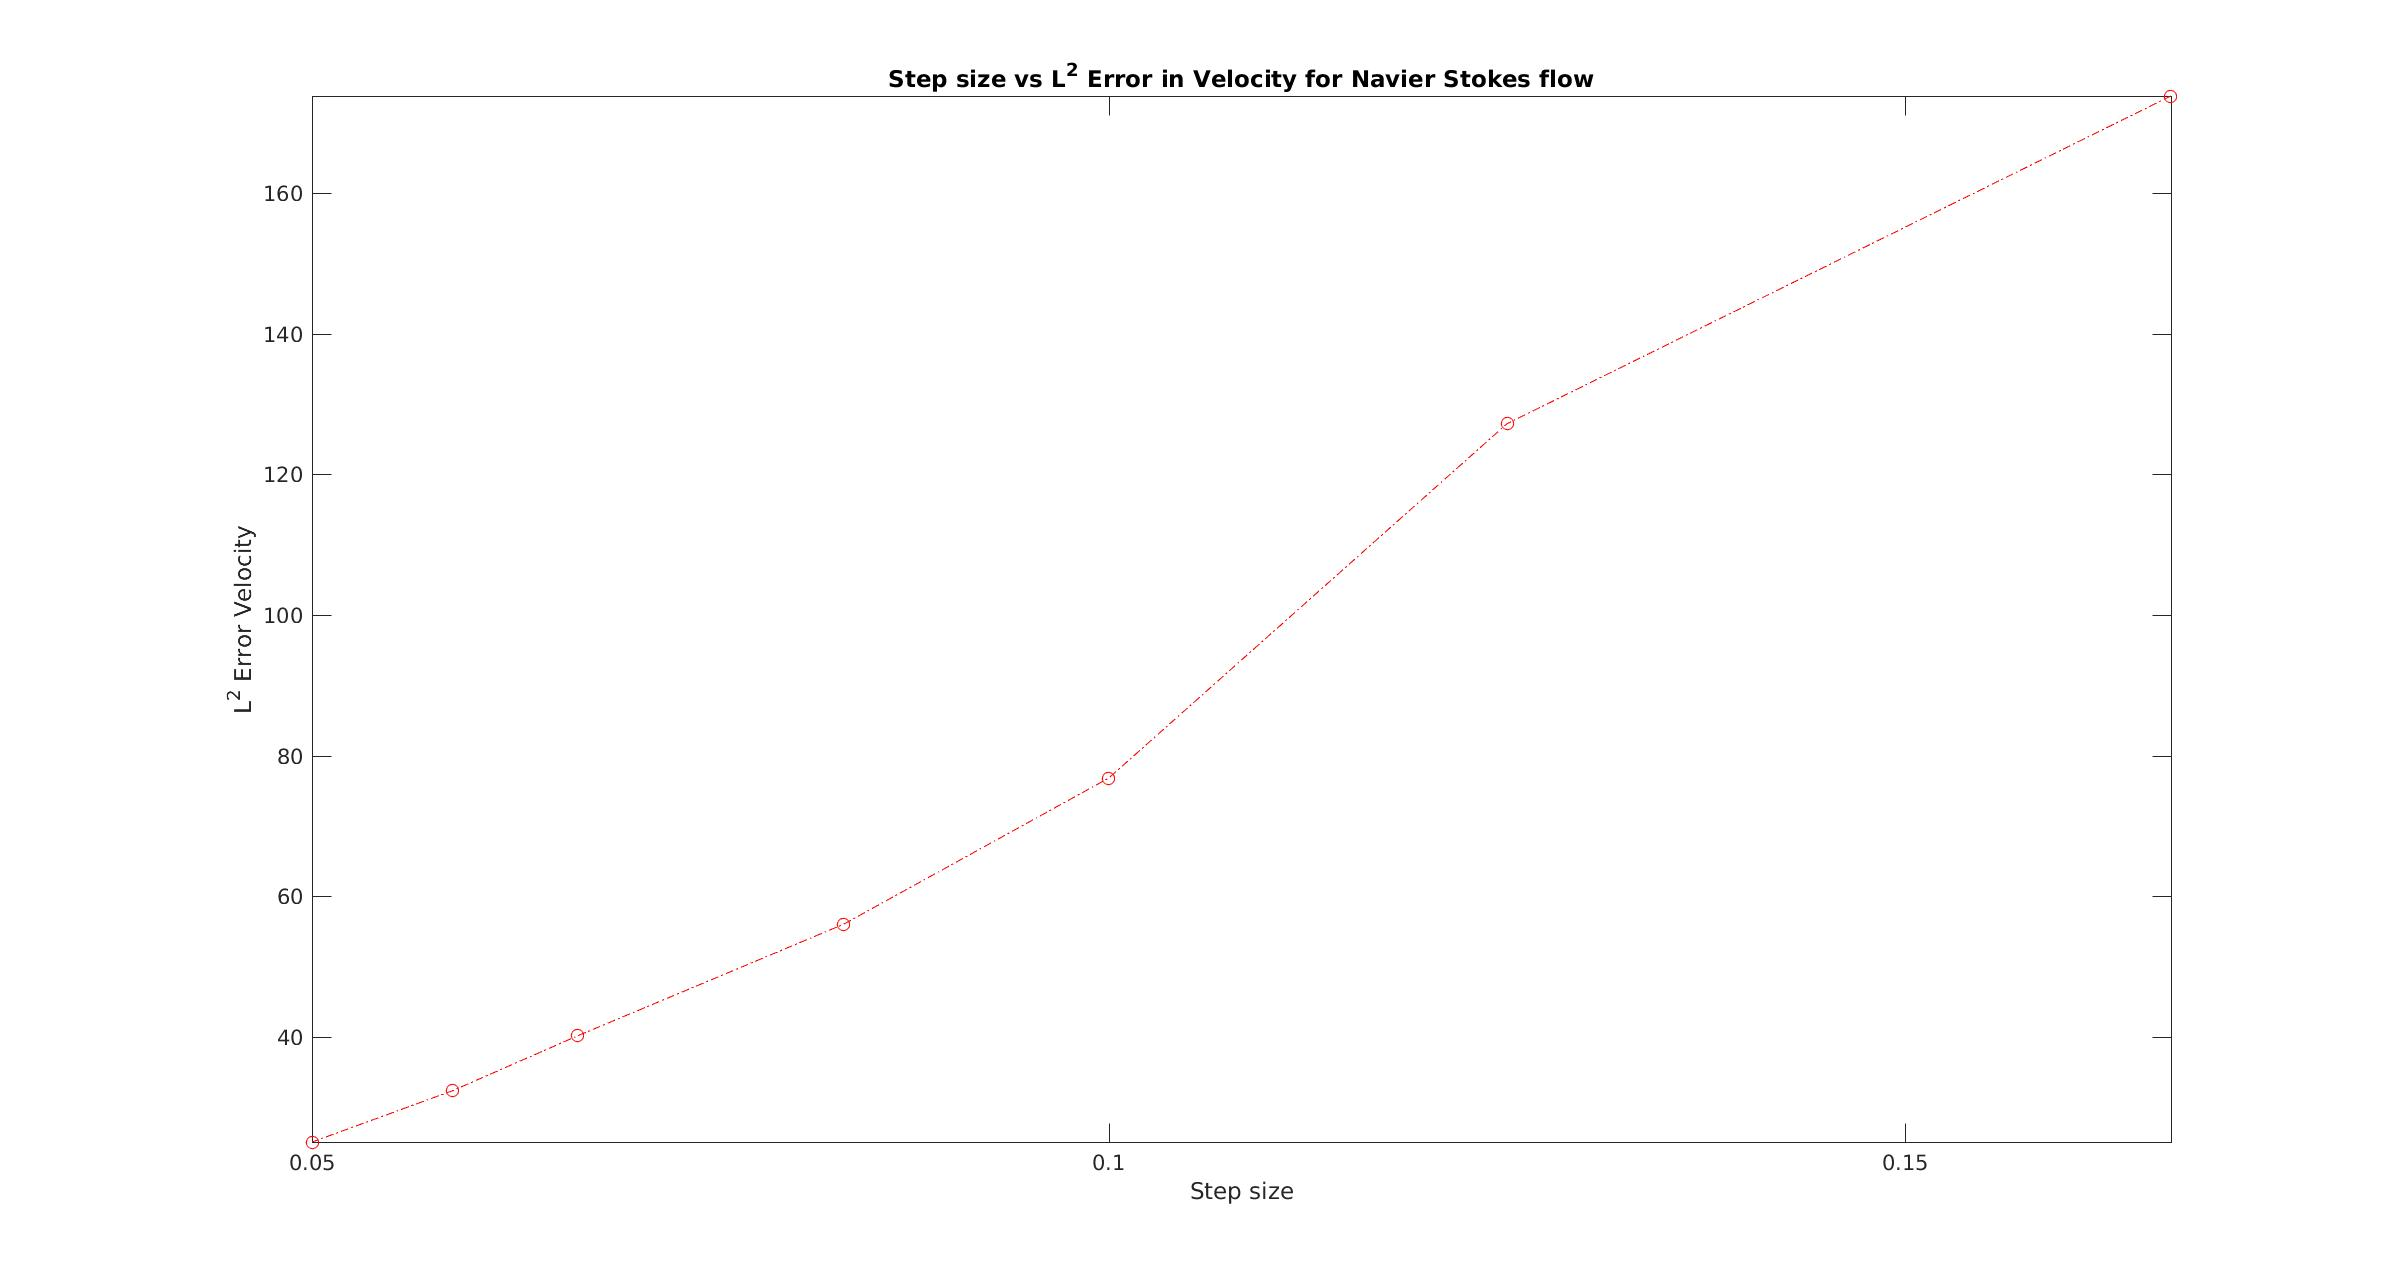
\includegraphics[width=\linewidth]{L2_convergence_velocity_n_s.jpg}
    \label{fig:vel_navier_stoke_conv}
\end{subfigure}
\caption{$h-$convergence test for velocity $L^2$ error}
\label{navier_stoke_conv_l2}
\end{figure}
\end{frame}
%------------------------------------------------
\begin{frame}
\frametitle{Navier-Stokes equation: Convergence test}
\begin{figure}
\begin{subfigure}{\textwidth}	
    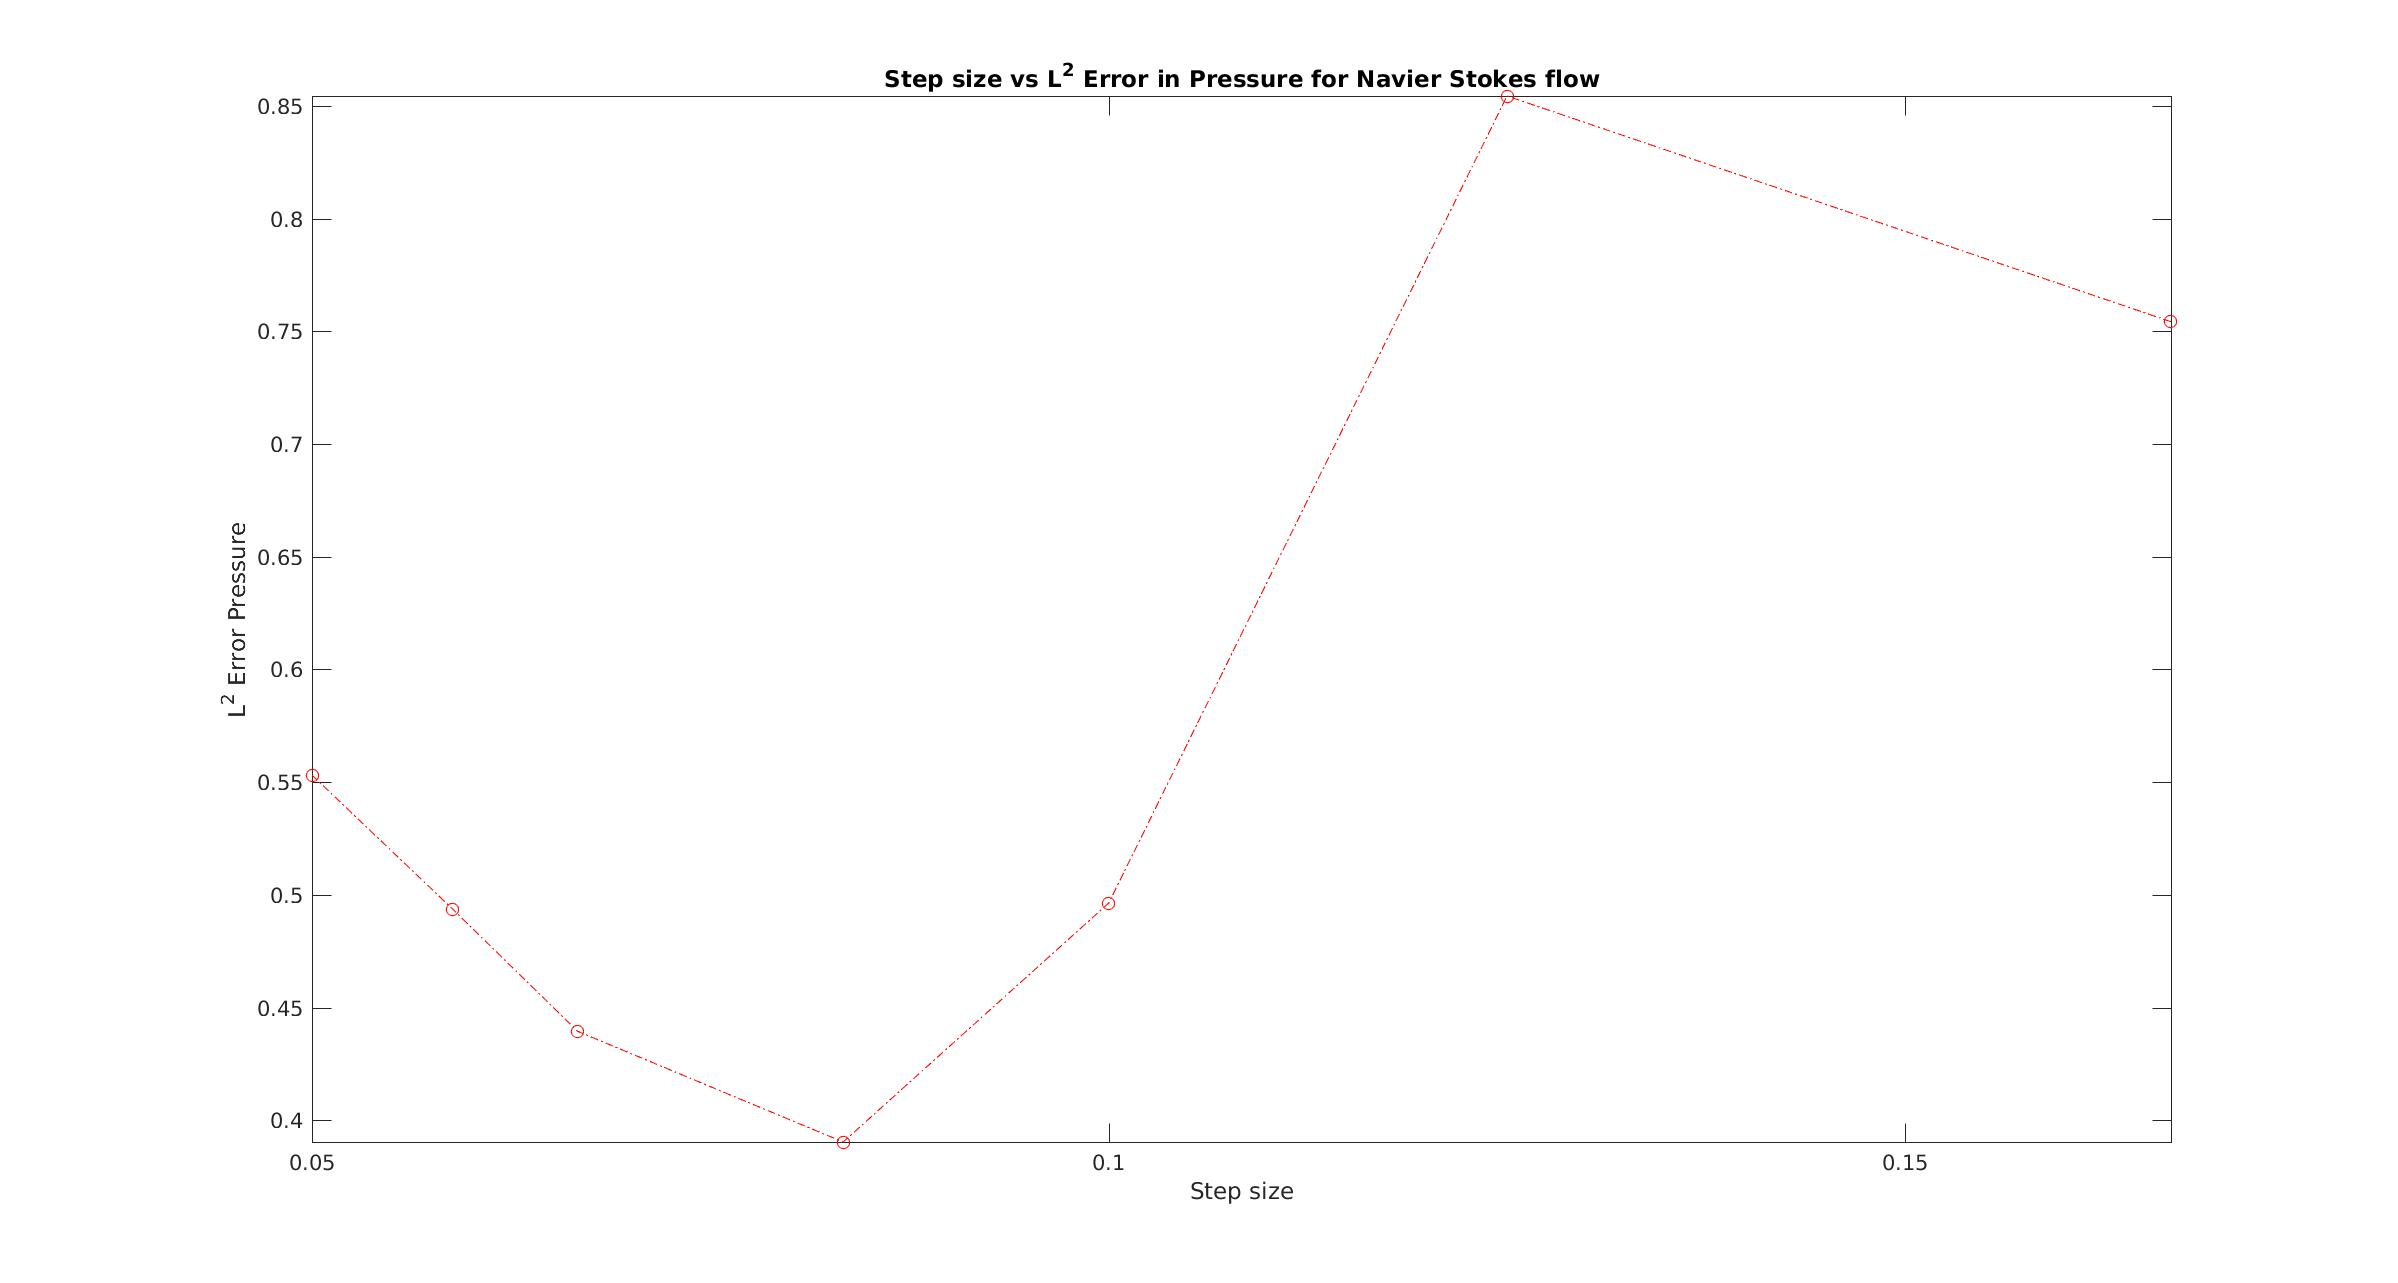
\includegraphics[width=\linewidth]{L2_convergence_pressure_n_s.jpg}
  \label{fig:pre_navier_stoke_conv}
\end{subfigure}
\caption{$h-$convergence test for pressure in $L^2$ error}
\label{navier_stoke_conv_l2}
\end{figure}
\end{frame}
%------------------------------------------------
\begin{frame}
\frametitle{Navier-Stokes equation: Convergence test}
\begin{figure}
\begin{subfigure}{0.8\textwidth}	
  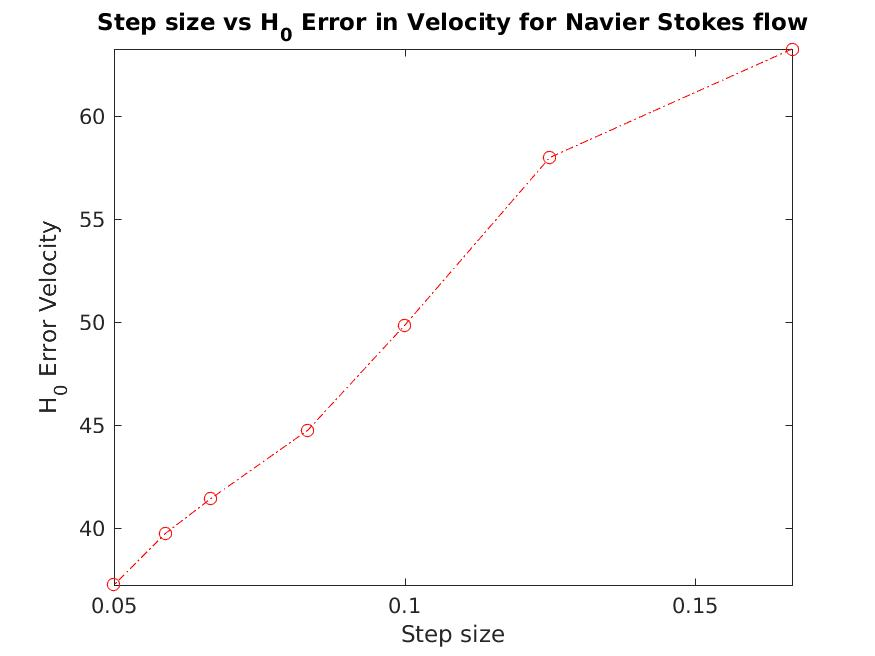
\includegraphics[width=0.8\linewidth]{H0_convergence_velocity_n_s.jpg}
  \label{fig:vel_navier_stoke_conv_h0}
\end{subfigure}
\caption{$h-$convergence test for velocity $H_0$ error}
\label{navier_stoke_conv_h0}
\end{figure}
\end{frame}
%------------------------------------------------
\begin{frame}
\frametitle{Navier-Stokes equation: Convergence test}
\begin{figure}
\begin{subfigure}{\textwidth}	
  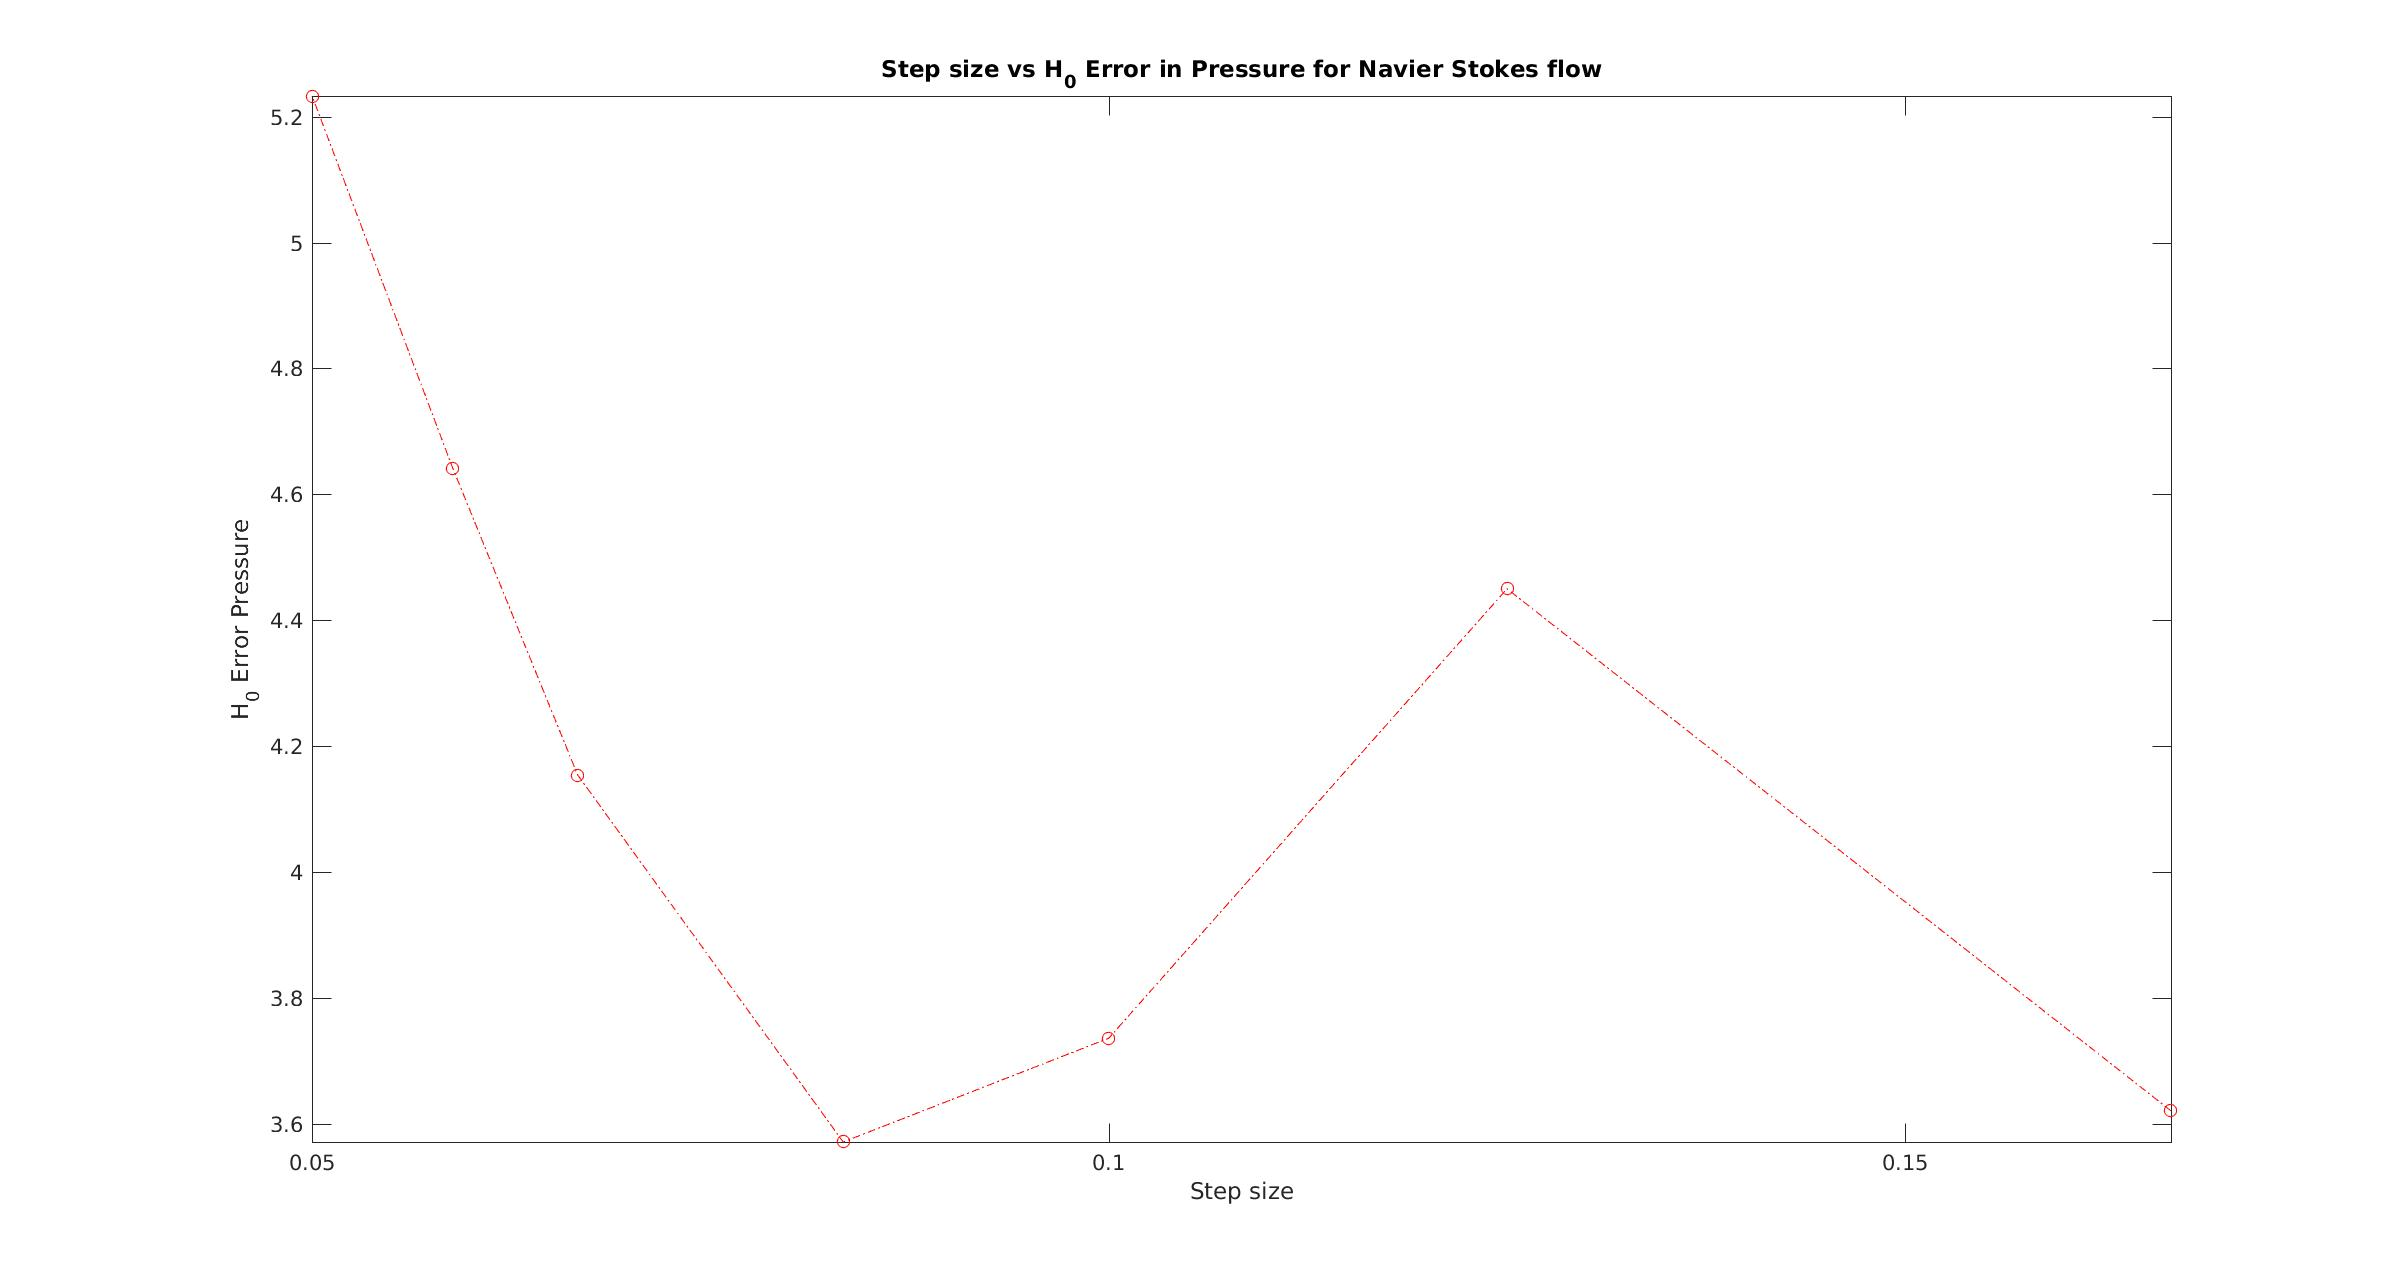
\includegraphics[width=\linewidth]{H0_convergence_pressure_n_s.jpg}
  \label{fig:pre_navier_stoke_conv_h0}
\end{subfigure}
\caption{$h-$convergence test for pressure in $H_0$ error}
\label{navier_stoke_conv_h0}
\end{figure}
\end{frame}
%------------------------------------------------
\begin{frame}
\frametitle{Navier-Stokes equation: Flow around cylinder}
\begin{figure}
  \begin{subfigure}{0.3\textwidth}
    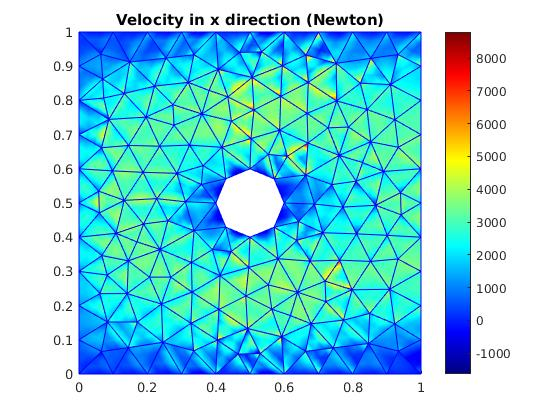
\includegraphics[width=\linewidth]{cylinder_newton_vx_schur.jpg}
    \caption{$x-$velocity}
  \label{x_vel_navier_stoke_schur}
  \end{subfigure}
  \begin{subfigure}{0.3\textwidth}
    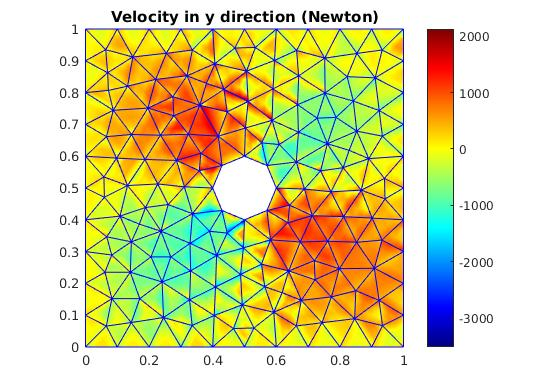
\includegraphics[width=\linewidth]{cylinder_newton_vy_schur.jpg}
    \caption{$y-$velocity}
  \label{y_vel_navier_stoke_schur}
  \end{subfigure}
  \begin{subfigure}{0.3\textwidth}
    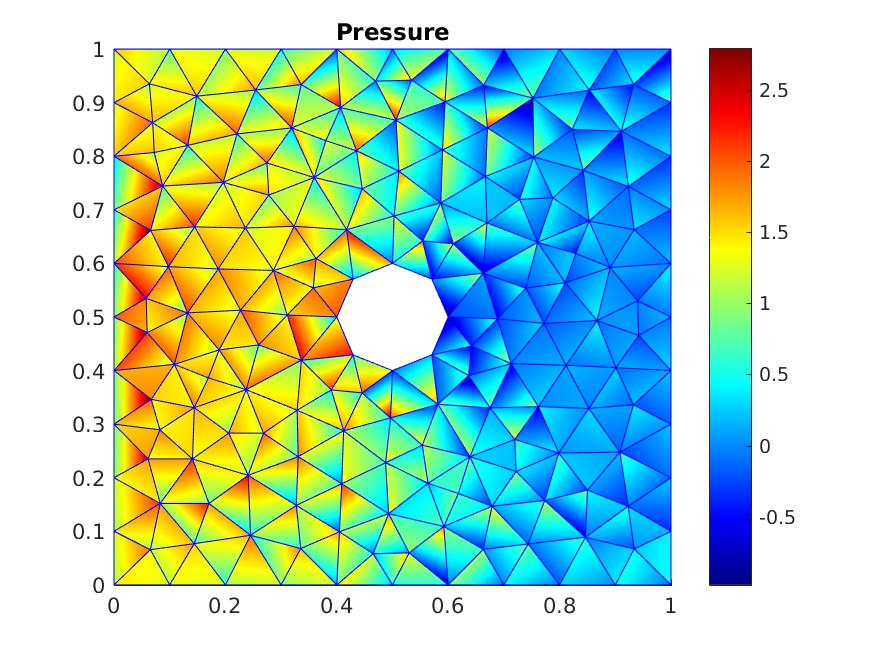
\includegraphics[width=\linewidth]{cylinder_newton_pressure_schur.jpg}
    \caption{Pressure}
  \label{pressure_navier_stoke_schur}
  \end{subfigure}
\caption{Flow over cylinder (Initial guess by Schur complement method)}
\label{flow_over_cylinder_schur_n_s}
\end{figure}
\end{frame}
%------------------------------------------------
\begin{frame}
\frametitle{Navier-Stokes equation: Lid driven cavity}
\begin{figure}
  \begin{subfigure}{0.3\textwidth}
    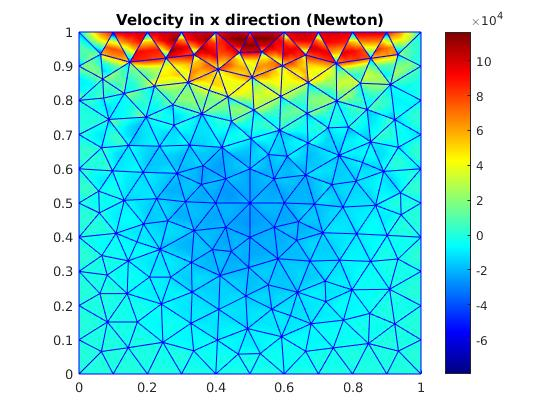
\includegraphics[width=\linewidth]{lid_newton_vx_schur.jpg}
    \caption{$x-$velocity}
  \label{x_vel_navier_stoke_schur_lid}
  \end{subfigure}
  \begin{subfigure}{0.3\textwidth}
    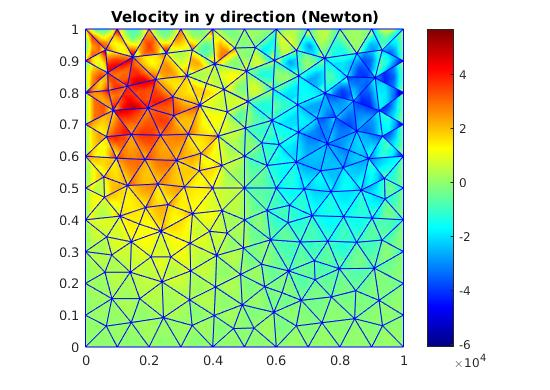
\includegraphics[width=\linewidth]{lid_newton_vy_schur.jpg}
    \caption{$y-$velocity}
  \label{y_vel_navier_stoke_schur_lid}
  \end{subfigure}
  \begin{subfigure}{0.3\textwidth}
    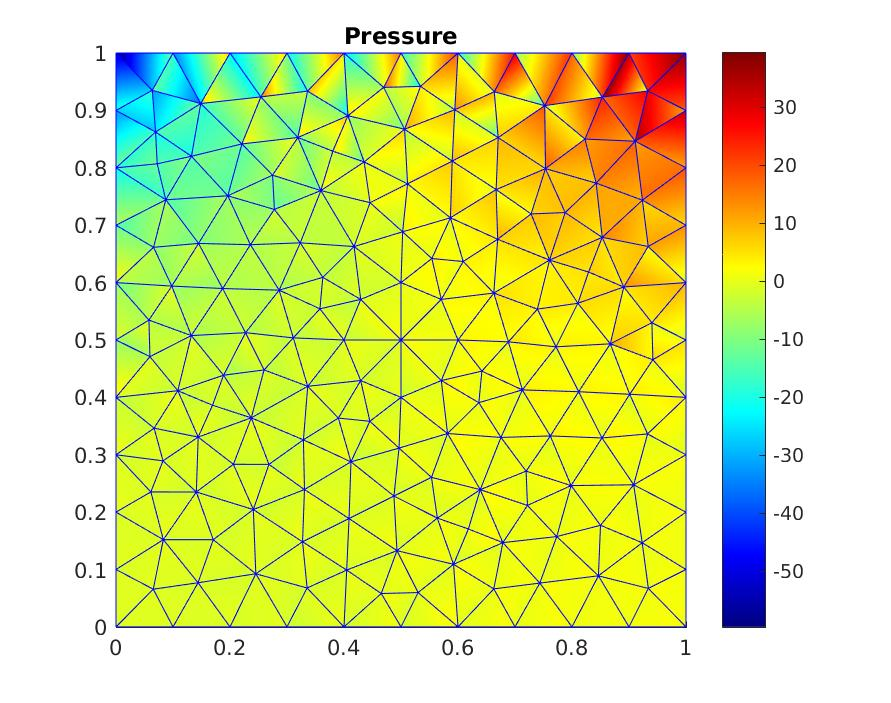
\includegraphics[width=\linewidth]{lid_newton_pressure_schur.jpg}
    \caption{Pressure}
  \label{pressure_navier_stoke_schur_lid}
  \end{subfigure}
\caption{Lid driven cavity flow (Initial guess by Schur complement method)}
\label{lid_driven_cavity_n_s_schur}
\end{figure}
\end{frame}
%------------------------------------------------
\section{Conclusions and outlook}
%------------------------------------------------
\begin{frame}
\frametitle{Conclusions}

\begin{block}{Numerical considerations}
\begin{itemize}
\item The higher polynomial degree does not always guarantee better accuracy. However, the convergence rate increases with increase in polynomial degree.
\item The initial guess, here, solution of the Stokes equation, is crucial for success of the Newton method for the Navier Stokes equation.
\item Convergence of solution.
\end{itemize}
\end{block}

\begin{block}{Solvers performance}
\begin{itemize}
\item The Schur complement method: Efficient and accurate.
\item The $minres$ solver : Slow convergence 
\item The $bicgstab$ : Convergence failure.
\end{itemize}
\end{block}

\end{frame}

%------------------------------------------------

\begin{frame}
\frametitle{Outlook}
\begin{block}{Discontinuous Galerkin method}
\begin{itemize}
\item Test for higher Reynold's number.
\item Further solvers/methods.
\item Time dependent cases.
\end{itemize}
\end{block}

\begin{block}{Model order reduction}
\begin{itemize}
\item Parametrization.
\item Reduced order modelling.
\end{itemize}
\end{block}


\end{frame}

%------------------------------------------------
\begin{frame}
\frametitle{References}
\bibliographystyle{plain}
\bibliography{ref1}


\end{frame}
\appendix
%------------------------------------------------

\begin{frame}
\frametitle{Notations}
$\Omega$ = Continuous domain,\\
$\Gamma_D$ = Dirichlet boundary, \\
$\Gamma_N$ = Neumann boundary, \\
$cv$ = Control volume,\\
$cs$ = Control surface,\\
$B'$ = Extensive quantity under consideration,\\
$b'$ = Intensive quantity corresponding to $B'$,\\
$u$ = flow velocity and $u:\Omega \rightarrow \mathbb{R}^d$,\\
$p$ = pressure and $p:\Omega \rightarrow \mathbb{R}$,\\
$\nu$ = kinematic viscocity (fluid property) and $\nu:\Omega \rightarrow \mathbb{R}$,\\ 
$f$ = external force and $f:\Omega \rightarrow \mathbb{R}^d$,\\
$u_D$ = specified flow velocity at Dirichlet boundary and $u_D:\Gamma_D \rightarrow \mathbb{R}^d$,\\
$n$ = normal unit vector and $n:\partial \Omega \rightarrow \mathbb{R}^d$,\\
$\rho$ = density (fluid property) and $\rho:\Omega \rightarrow \mathbb{R}$,\\
$t$ = specified Neumann flux and $t:\Gamma_N \rightarrow \mathbb{R}^d$.\\
\end{frame}
%------------------------------------------------
\begin{frame}
\frametitle{Grid}
\begin{figure}
\begin{subfigure}{0.45\textwidth}
\centering
  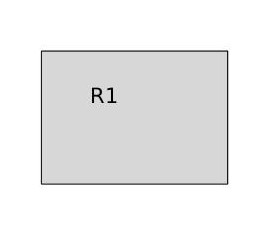
\includegraphics[width=\linewidth]{domain.jpg}
  \label{fig:Domain}
\end{subfigure}
\begin{subfigure}{0.45\textwidth}	
\centering
  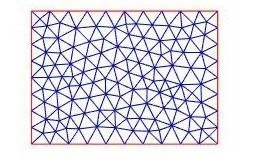
\includegraphics[width=\linewidth]{grid.jpg}
  \label{fig:Mesh}
\end{subfigure}
\caption{Continuous domain (left) and discretised domain or grid (right)}
\label{fig:continuous_grid_figure}
\end{figure}

\end{frame}

%------------------------------------------------
\begin{frame}
\frametitle{Grid}
\begin{figure}
\centering
  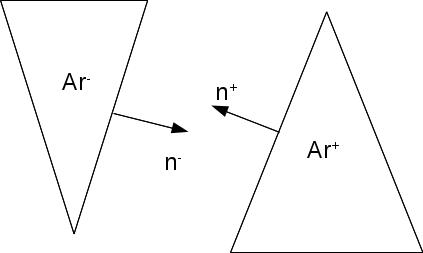
\includegraphics[width=0.9\linewidth]{ch_3_fig_1.jpg}
  \caption{Element self (+) and neighbouring element (-)}
  \label{fig:Self_neighbour}
\end{figure}

\end{frame}

%------------------------------------------------
\begin{frame}
\frametitle{Global and local coordinate system}
\begin{itemize}

\item The transformation from local coordinate $\hat{X}$ to global coordinate $X$ is defined by the mapping,
\begin{equation}\label{local global mapping}
\begin{split}
F_k:\hat{X} \mapsto X \quad \forall \quad \hat{X} \in \hat{T} \quad \textrm{and} \quad X \in \mathcal{T} \\
F_k(\hat{X}): X = J_k \hat{X} + C
\end{split}
\end{equation}

\begin{figure}[0.6\textwidth]
\begin{picture}(300,100)(0,0) 
\put(0,0){\line(1,0){50}}
\put(50,0){\line(1,1){100}}
\put(0,0){\line(3,2){150}}
\put(200,0){\line(1,0){100}}
\put(300,0){\line(-1,1){100}}
\put(200,100){\line(0,-1){100}}
\end{picture}
\end{figure}
\begin{center}
Global geometry (left) to Local geometry (right)
\end{center}

\end{itemize}

\end{frame}

%------------------------------------------------
\begin{frame}
\frametitle{Matrix assemblies}
\begin{block}{Assembly of $([n \otimes \phi], [n \otimes \phi])_{\Gamma \cup \Gamma_D}$}
Step 1 :
\begin{equation}
\begin{split}
res_1^{++} = (n \otimes \hat{\phi})^+ (n \otimes \hat{\phi})^+ \textrm{,}\\
res_1^{+-} = (n \otimes \hat{\phi})^+ (n \otimes \hat{\phi})^- \textrm{,}\\
res_1^{-+} = (n \otimes \hat{\phi})^- (n \otimes \hat{\phi})^+ \textrm{,}\\
res_1^{--} = (n \otimes \hat{\phi})^- (n \otimes \hat{\phi})^- \textrm{.}\\
\end{split}
\end{equation}
 
Step 2 : 
\begin{equation}
\begin{split}
res_2^{++} = \int_{\Gamma} res_1^{++} EL(i,j) \textrm{,}\\
res_2^{+-} = \int_{\Gamma} res_1^{+-} EL(i,j) \textrm{,}\\
\end{split}
\end{equation}
\end{block}
\end{frame}
%------------------------------------------------
\begin{frame}
\frametitle{Matrix assemblies}

\begin{block}{Assembly of $([n \otimes \phi], [n \otimes \phi])_{\Gamma \cup \Gamma_D}$}

\begin{equation}
\begin{split}
res_2^{-+} = \int_{\Gamma} res_1^{-+} EL(i,j) \textrm{,}\\
res_2^{--} = \int_{\Gamma} res_1^{--} EL(i,j) \textrm{.}\\
\end{split}
\end{equation}

Step 3 :
\begin{equation}
\begin{split}
res_3^{++}[ids\_velocity\_self,ids\_velocity\_self] = res_2^{++} \textrm{,}\\
res_3^{+-}[ids\_velocity\_self,ids\_velocity\_neighbour] = res_2^{+-} \textrm{,}\\
res_3^{-+}[ids\_velocity\_neighbour,ids\_velocity\_self] = res_2^{-+} \textrm{,}\\
res_3^{--}[ids\_velocity\_neighbour,ids\_velocity\_neighbour] = res_2^{--} \textrm{.}\\
\end{split}
\end{equation}

\begin{equation}
res_3 = res_3^{++} + res_3^{+-} + res_3^{-+} + res_3^{--} \textrm{.}
\end{equation}

\end{block}

\end{frame}

%------------------------------------------------
\begin{frame}
\frametitle{Program flow}
\begin{itemize}

\item Grid preparation
\item Fomrulating function space
\item Matrix assembly
\item Solving assembled form
\item Post processing
\item Newton method

\end{itemize}


\end{frame}

%------------------------------------------------

\begin{frame}
\frametitle{Stokes equation: Convergence test}
\begin{figure}
\begin{subfigure}{0.4\textwidth}	
  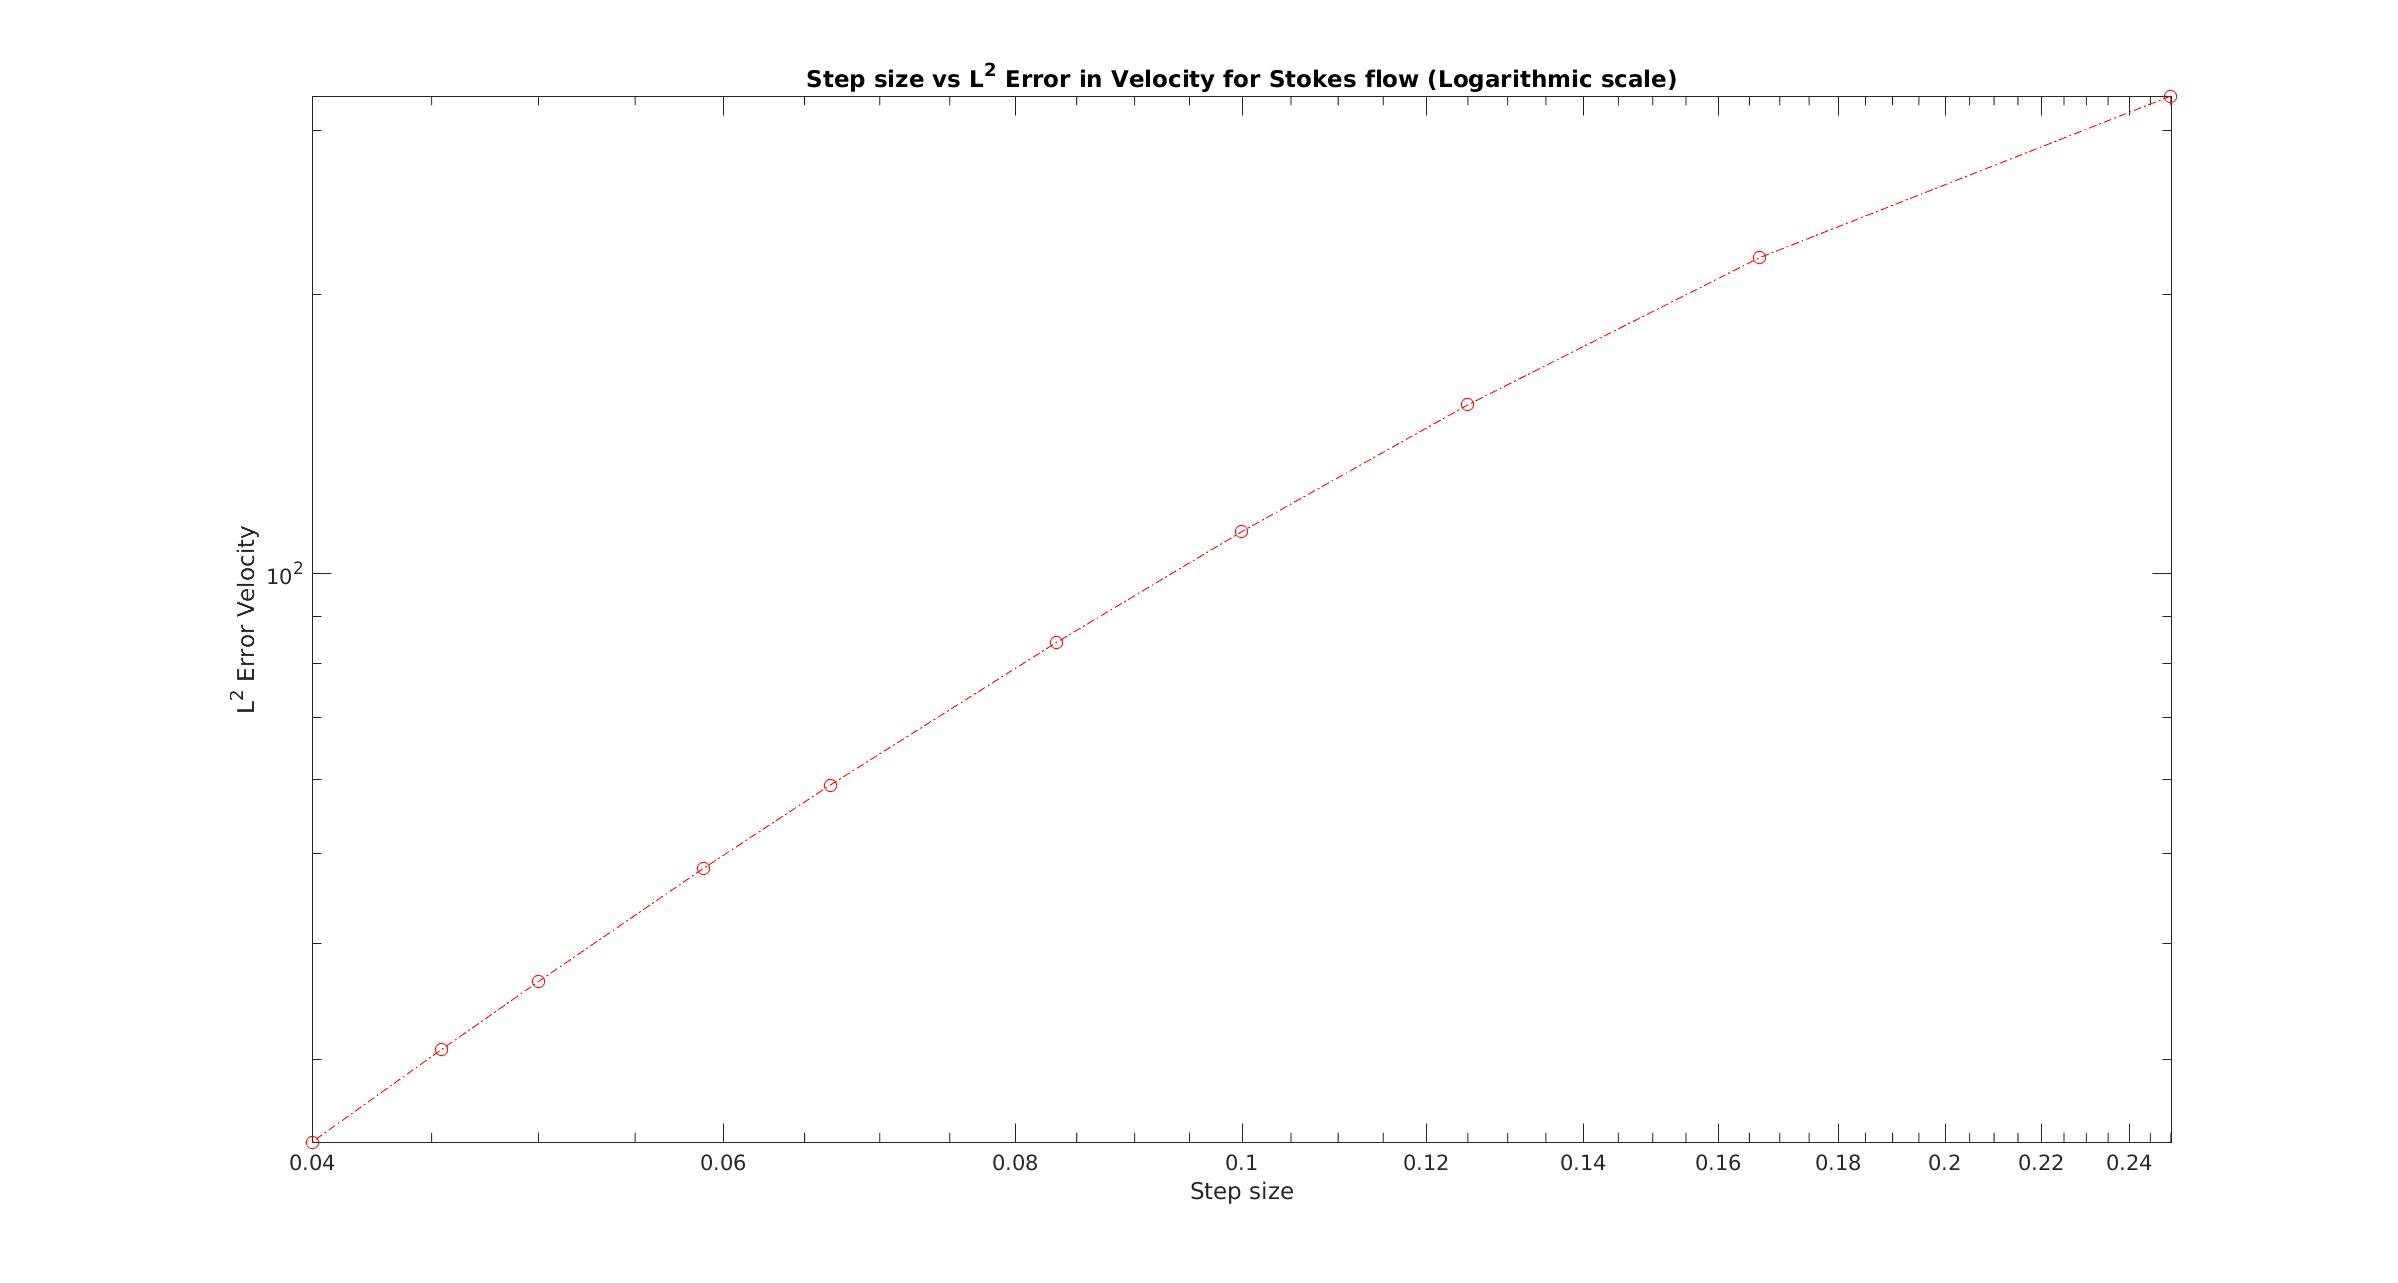
\includegraphics[width=\linewidth]{l2_velocity_log_stokes.jpg}
  \caption{$h-$convergence test for velocity $L^2$ error (Logarithmic scale)}
  \label{fig:vel_stoke_conv_log}
\end{subfigure}
\begin{subfigure}{0.4\textwidth}	
  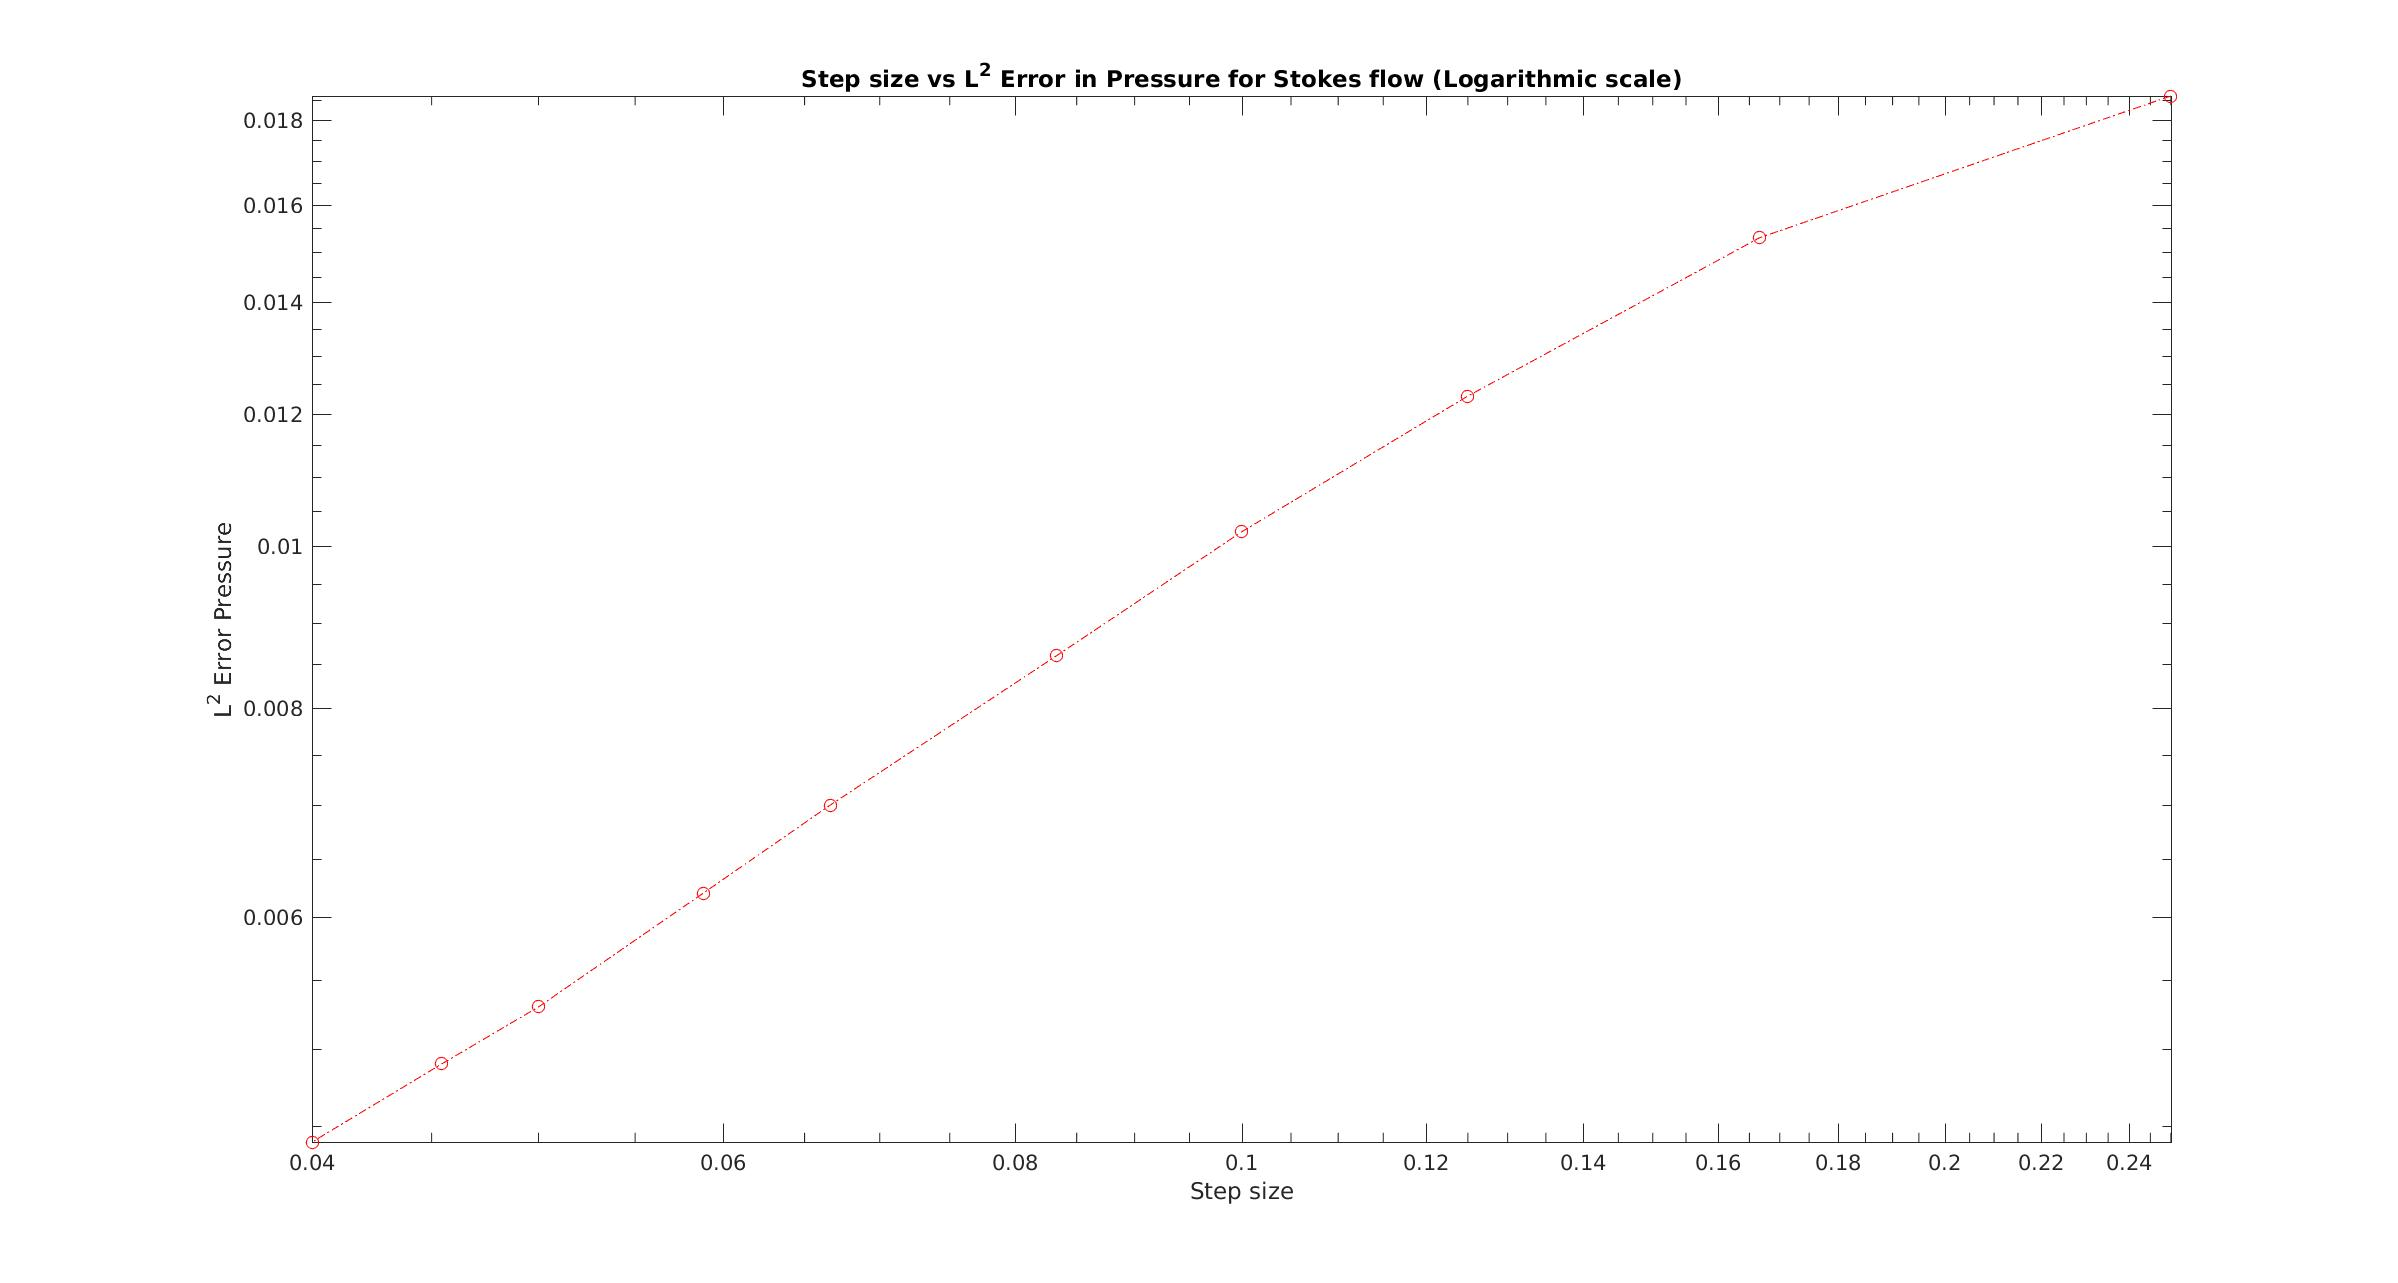
\includegraphics[width=\linewidth]{l2_pressure_log_stokes.jpg}
  \caption{$h-$convergence test for pressure in $L^2$ error (Logarithmic scale)}
  \label{fig:pre_stoke_conv_log}
\end{subfigure}
\caption{$h-$convergence in $L^2$ norm for the Stokes flow (Logarithmic scale)}
\label{fig:l2_stokes}
\end{figure}
\end{frame}
%------------------------------------------------
\begin{frame}
\frametitle{Stokes equation: Convergence test}
\begin{figure}
\begin{subfigure}{0.4\textwidth}	
  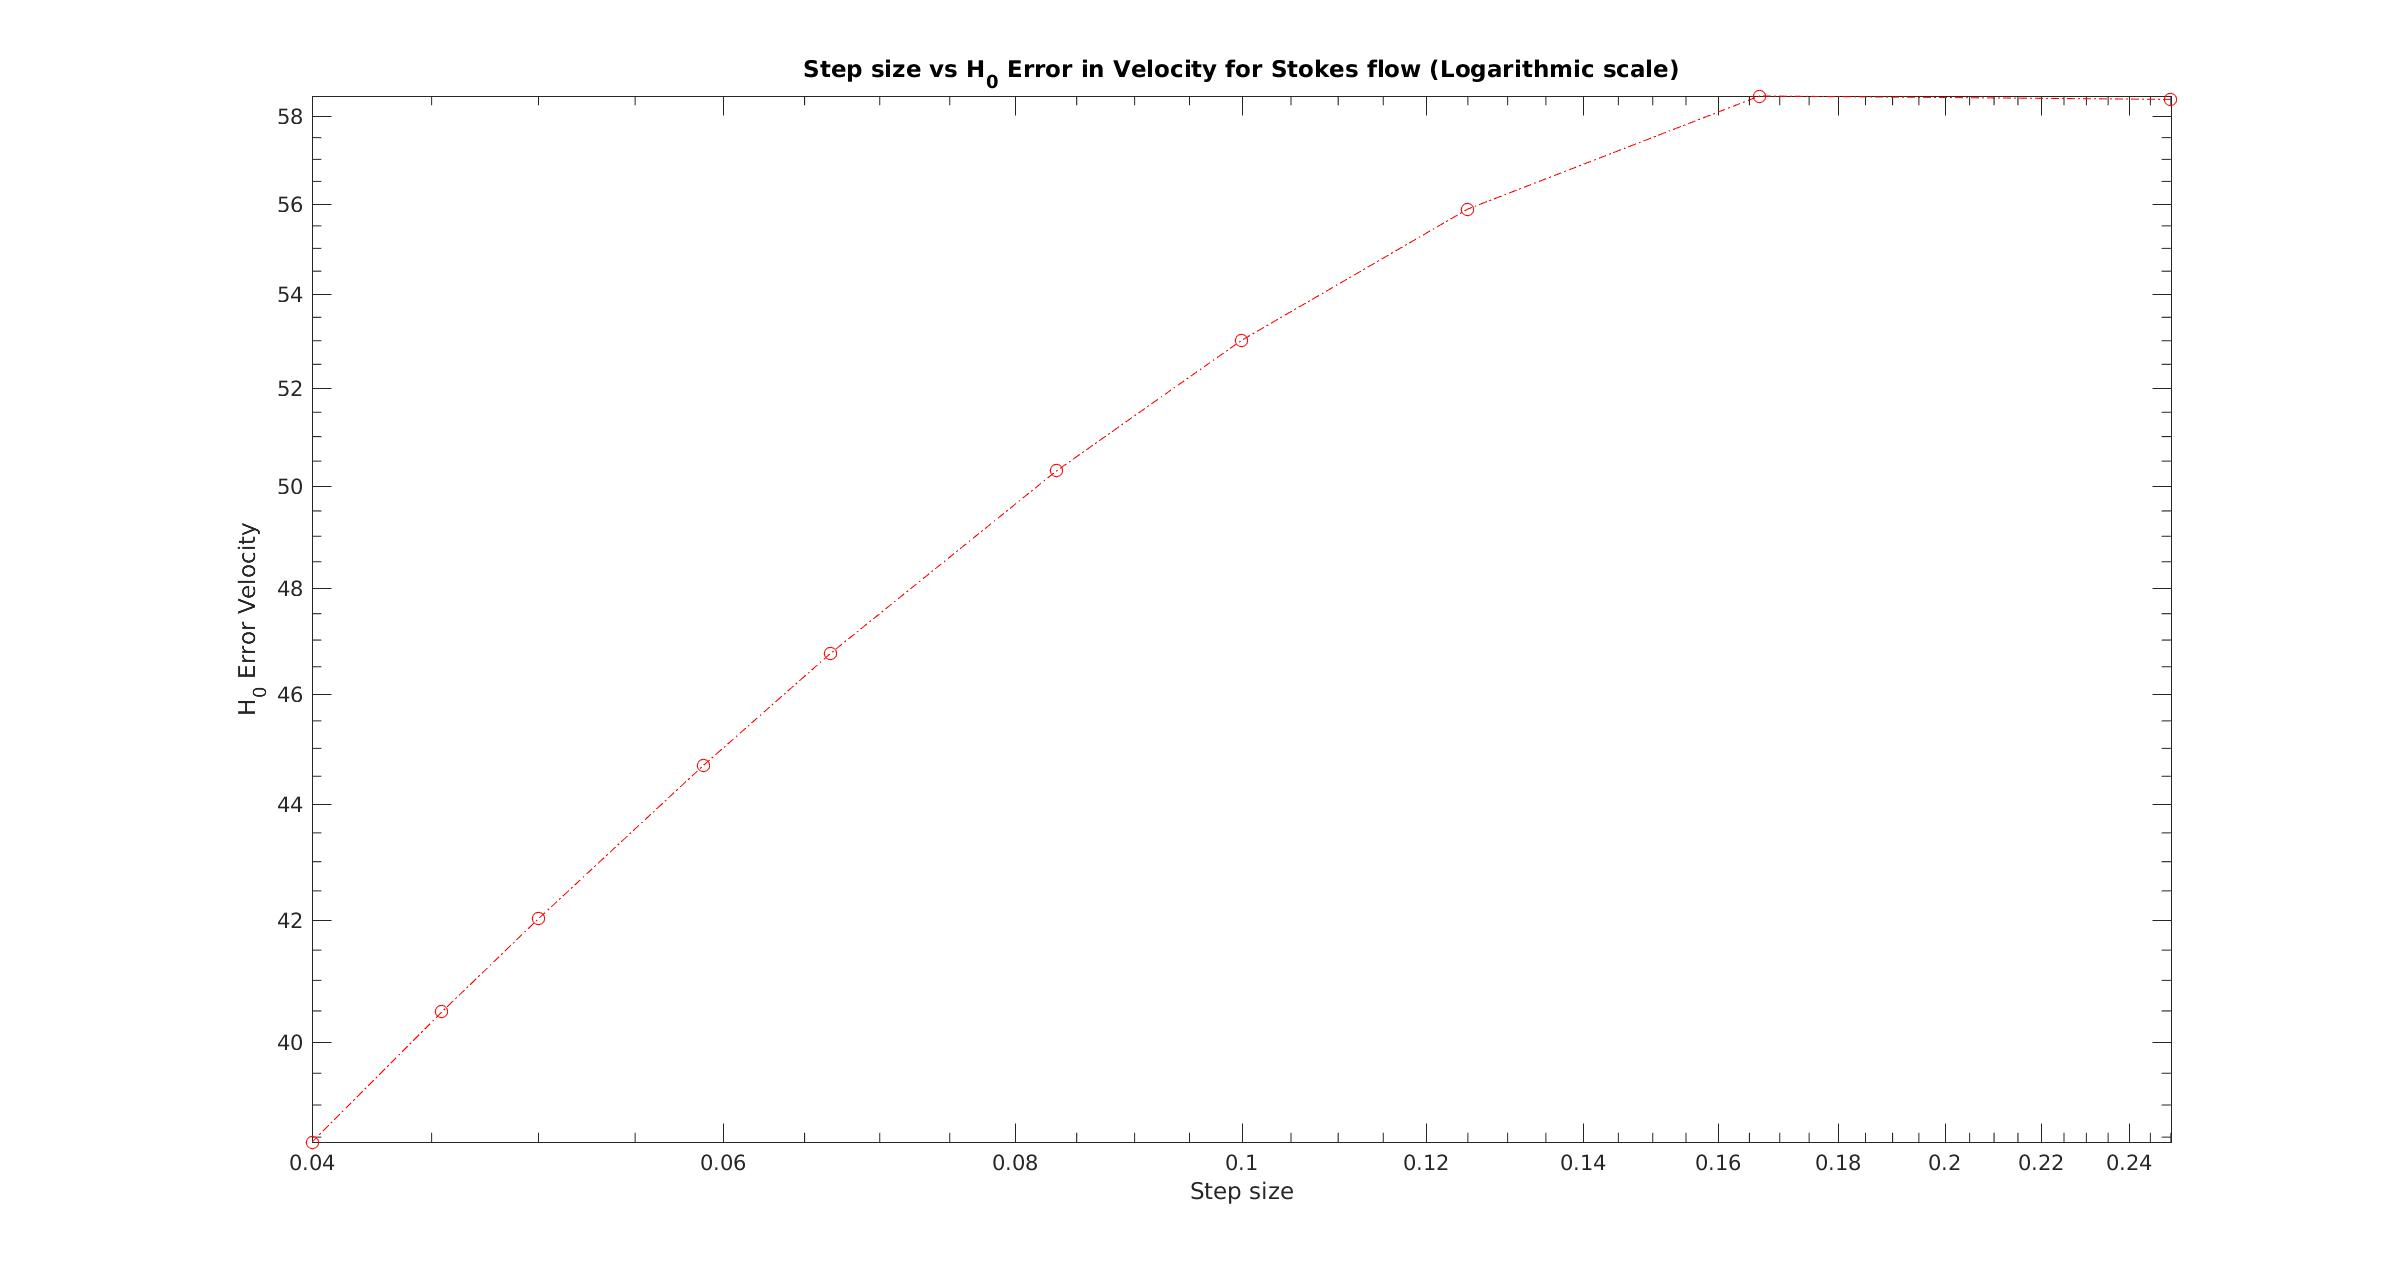
\includegraphics[width=\linewidth]{h0_velocity_log_stokes.jpg}
  \caption{$h-$convergence test for velocity $H_0$ error (Logarithmic scale)}
  \label{fig:vel_stoke_conv_log_h0}
\end{subfigure}
\begin{subfigure}{0.4\textwidth}	
  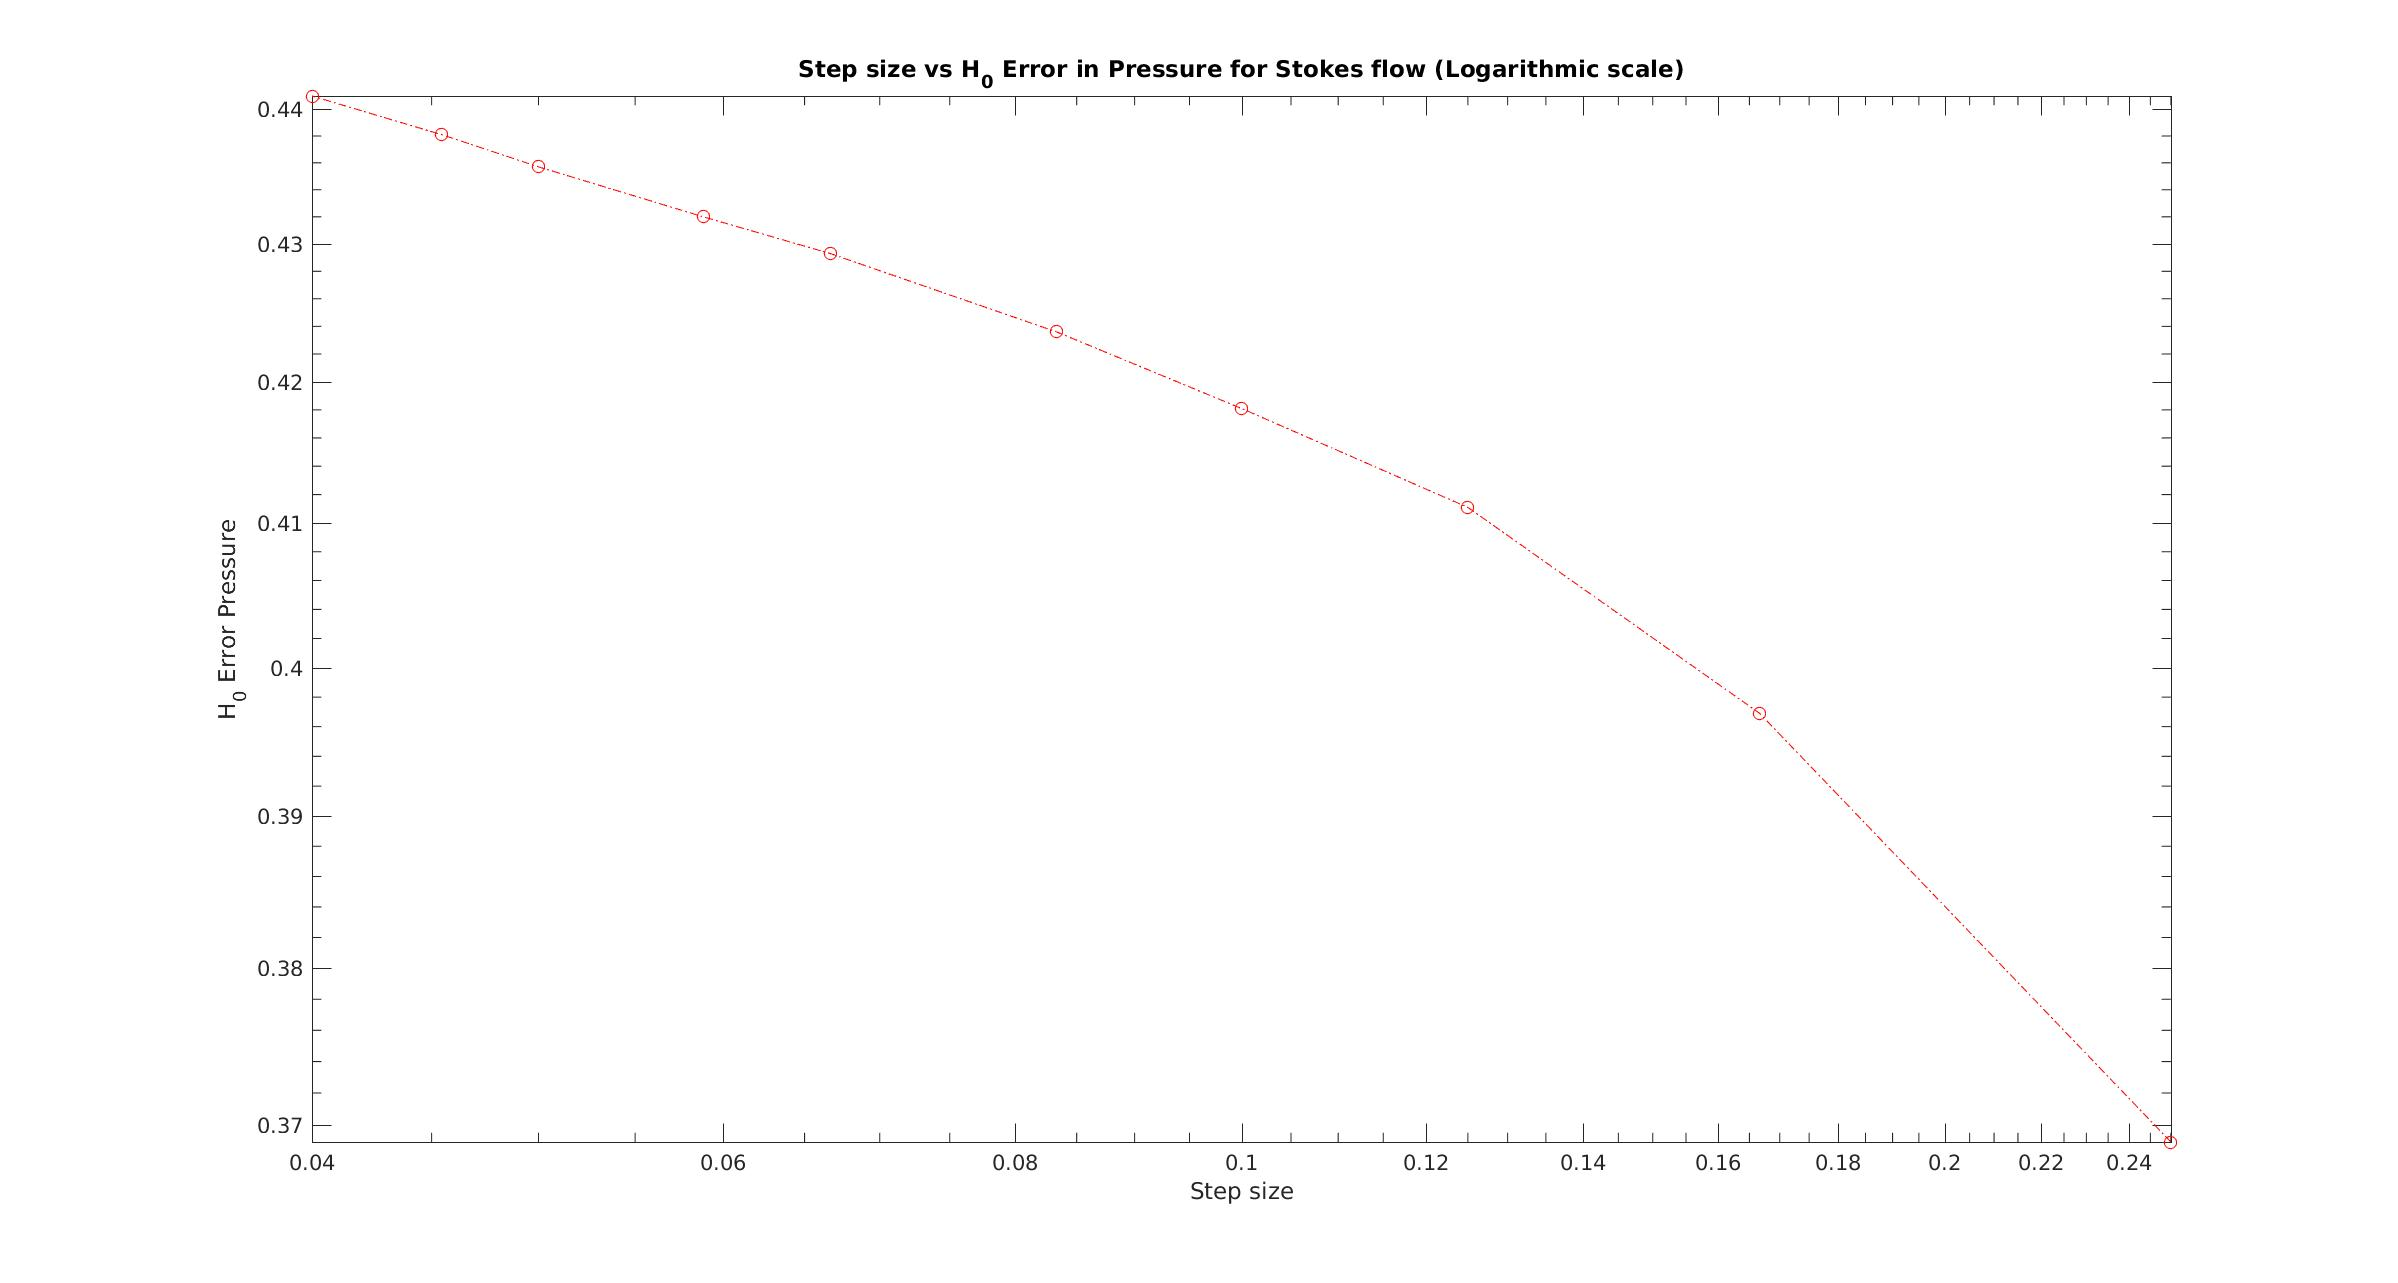
\includegraphics[width=\linewidth]{h0_pressure_log_stokes.jpg}
  \caption{$h-$convergence test for pressure in $H_0$ error (Logarithmic scale)}
  \label{fig:pre_stoke_conv_log_h0}
\end{subfigure}
\caption{$h-$convergence in $H_0$ norm for the Stokes flow (Logarithmic scale)}
\label{fig:h0_stokes}
\end{figure}
\end{frame}
%------------------------------------------------
\begin{frame}
\frametitle{Stokes equation: Lid driven cavity}
\begin{figure}
\begin{subfigure}{0.3\textwidth}	
  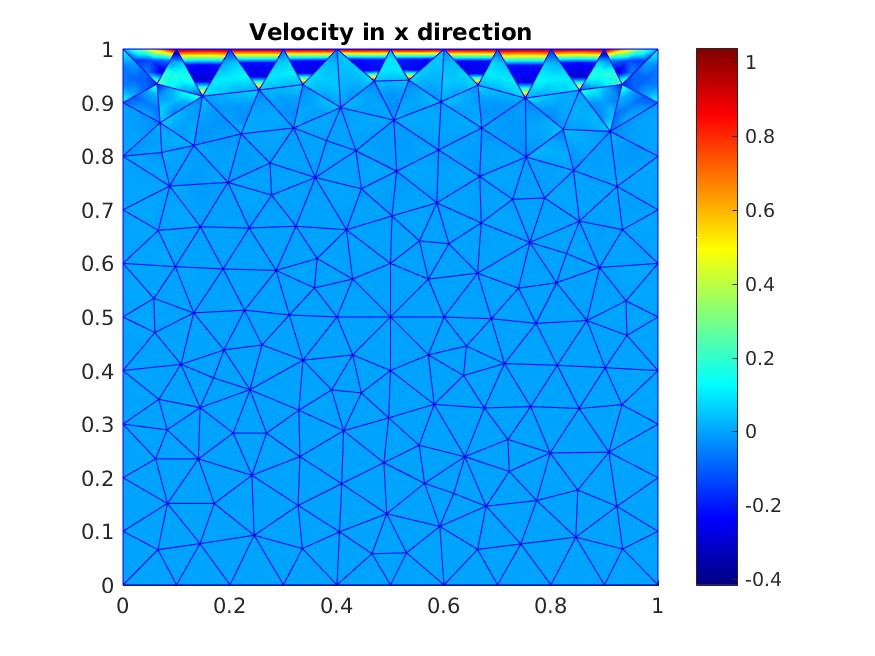
\includegraphics[width=\linewidth]{lid_minres_vx.jpg}
  \caption{$x-$velocity} 
  \label{x_vel_stoke_minres_lid}
\end{subfigure}
\begin{subfigure}{0.3\textwidth}	
  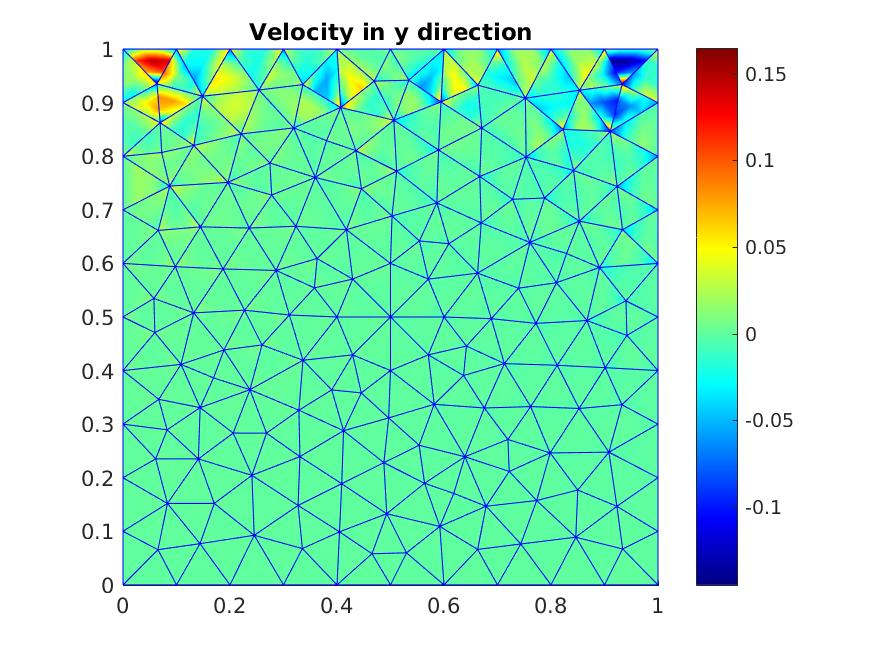
\includegraphics[width=\linewidth]{lid_minres_vy.jpg}
  \caption{$y-$velocity} 
  \label{y_vel_stoke_minres_lid}
\end{subfigure}
\begin{subfigure}{0.3\textwidth}	
  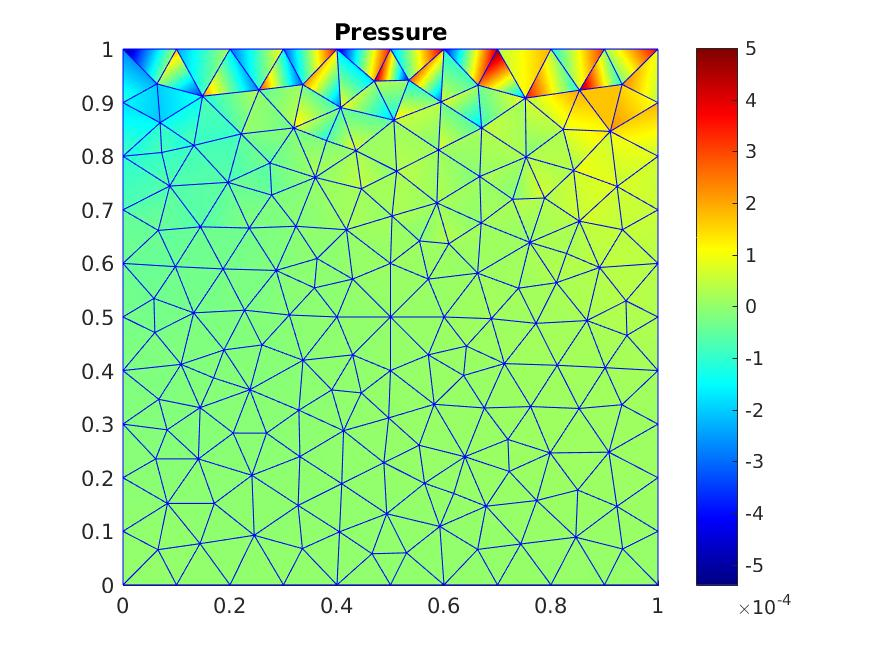
\includegraphics[width=\linewidth]{lid_minres_pressure.jpg}
  \caption{Pressure} 
  \label{pressure_stoke_minres_lid}
\end{subfigure}
\caption{Lid driven cavity problem ($minres$ solver)}
\label{stoke_minres_lid}
\end{figure}
\end{frame}
%------------------------------------------------
\begin{frame}
\frametitle{Navier-Stokes equation: Convergence test}
\begin{figure}
\begin{subfigure}{0.4\textwidth}	
  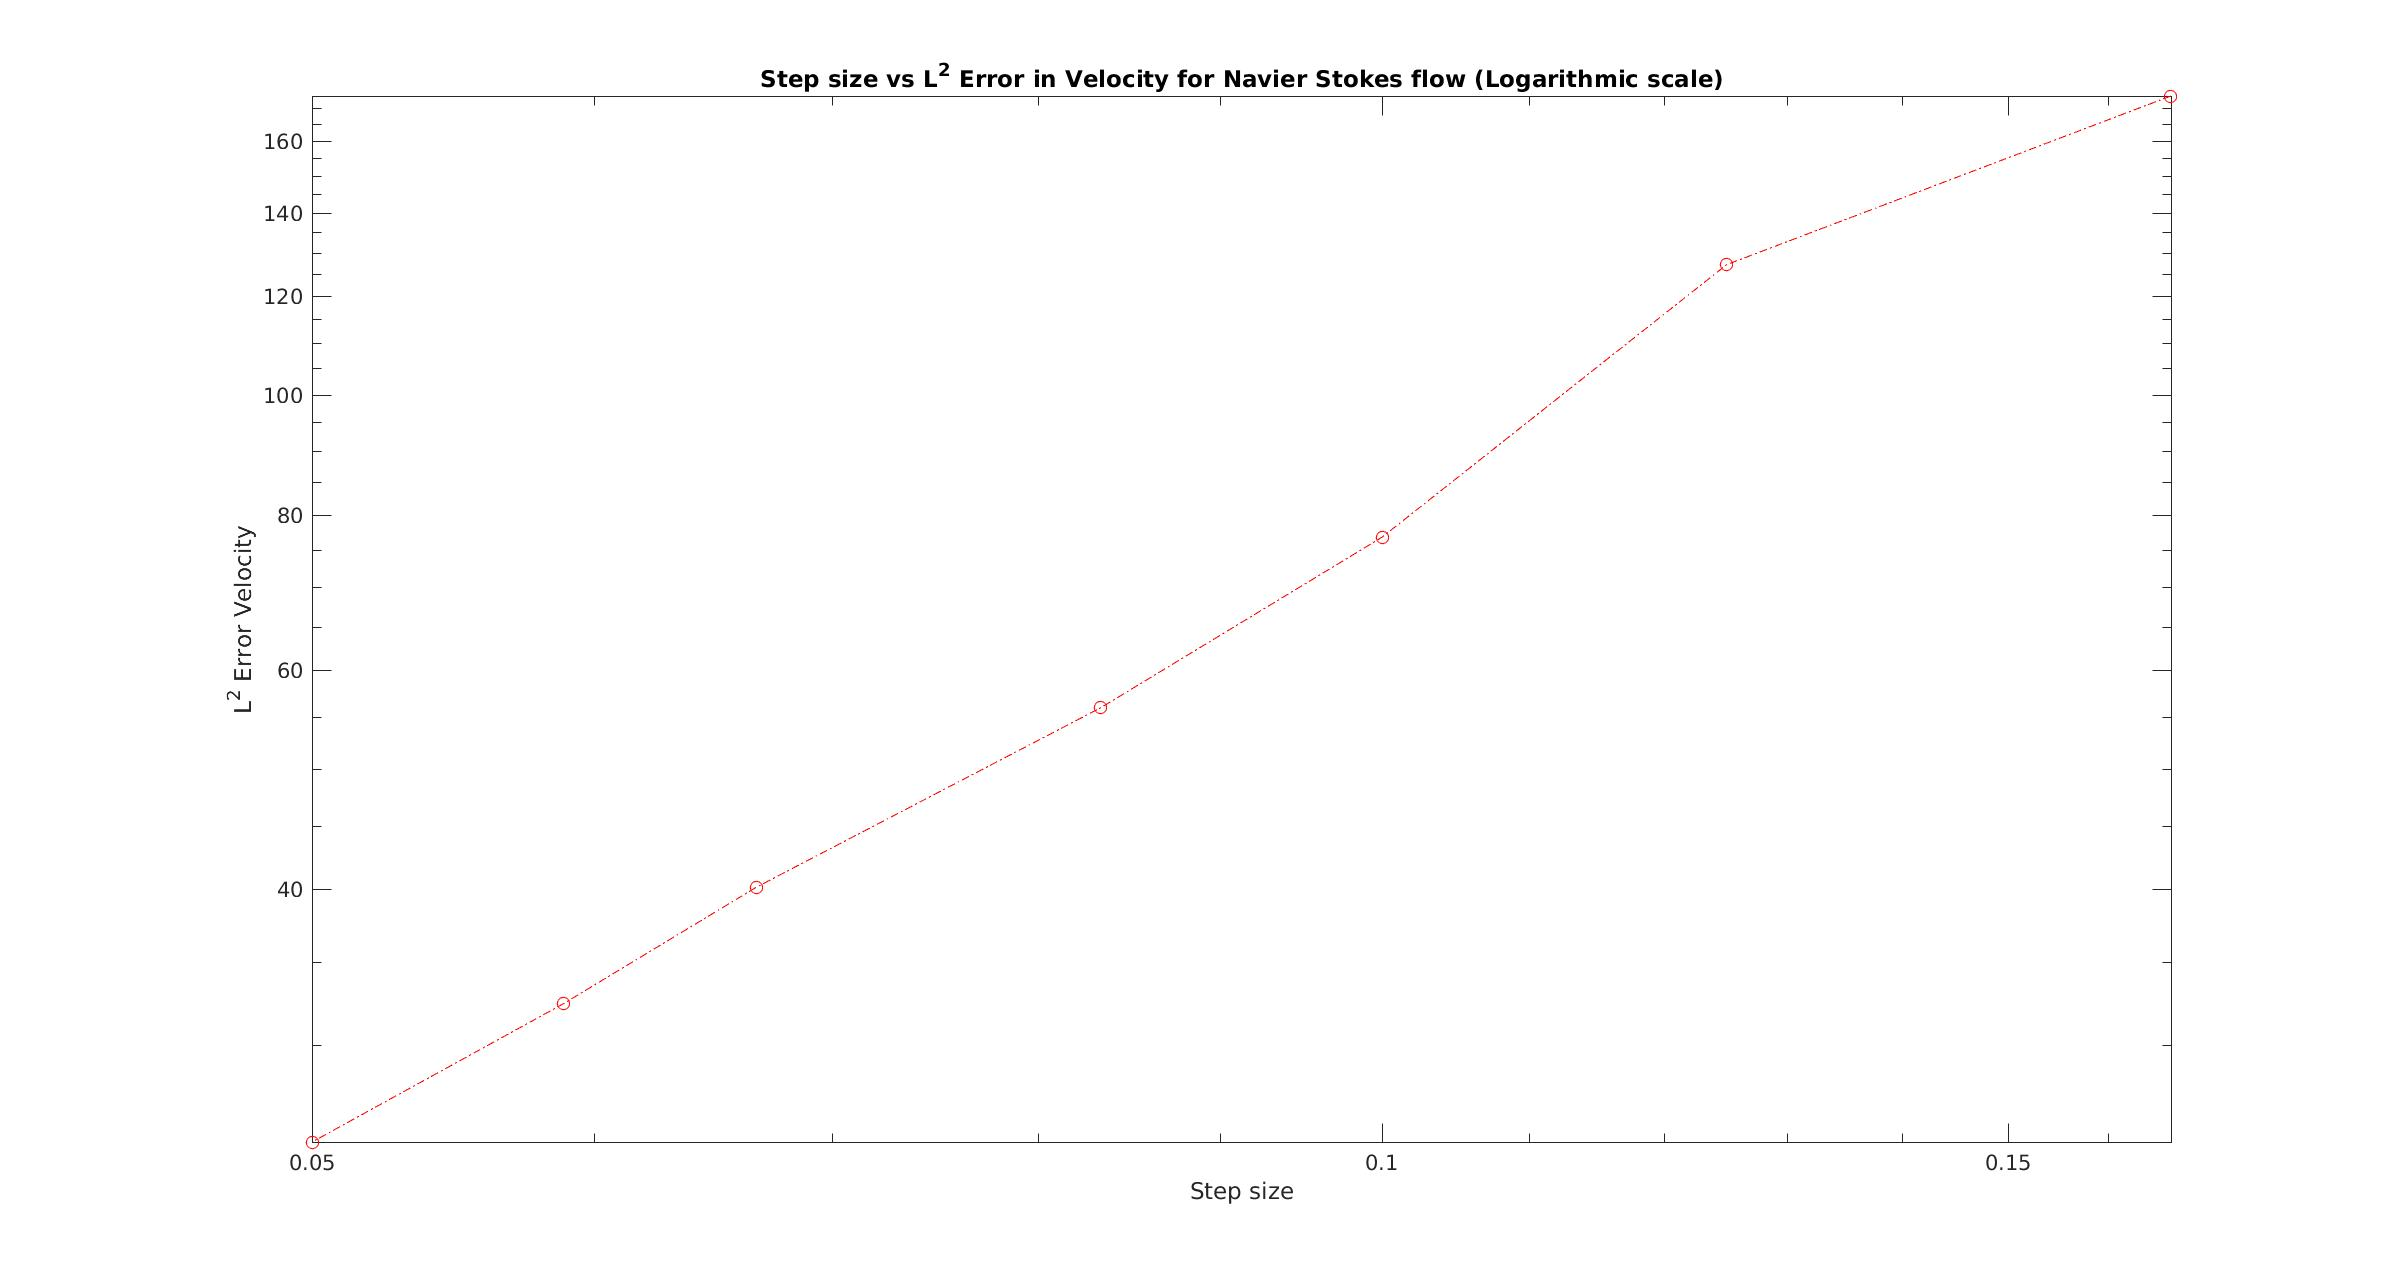
\includegraphics[width=\linewidth]{L2_convergence_velocity_n_s_log.jpg}
  \caption{$h-$convergence test for velocity $L^2$ error (Logarithmic scale)}
  \label{fig:vel_naviers_stoke_conv_log}
\end{subfigure}
\begin{subfigure}{0.4\textwidth}	
  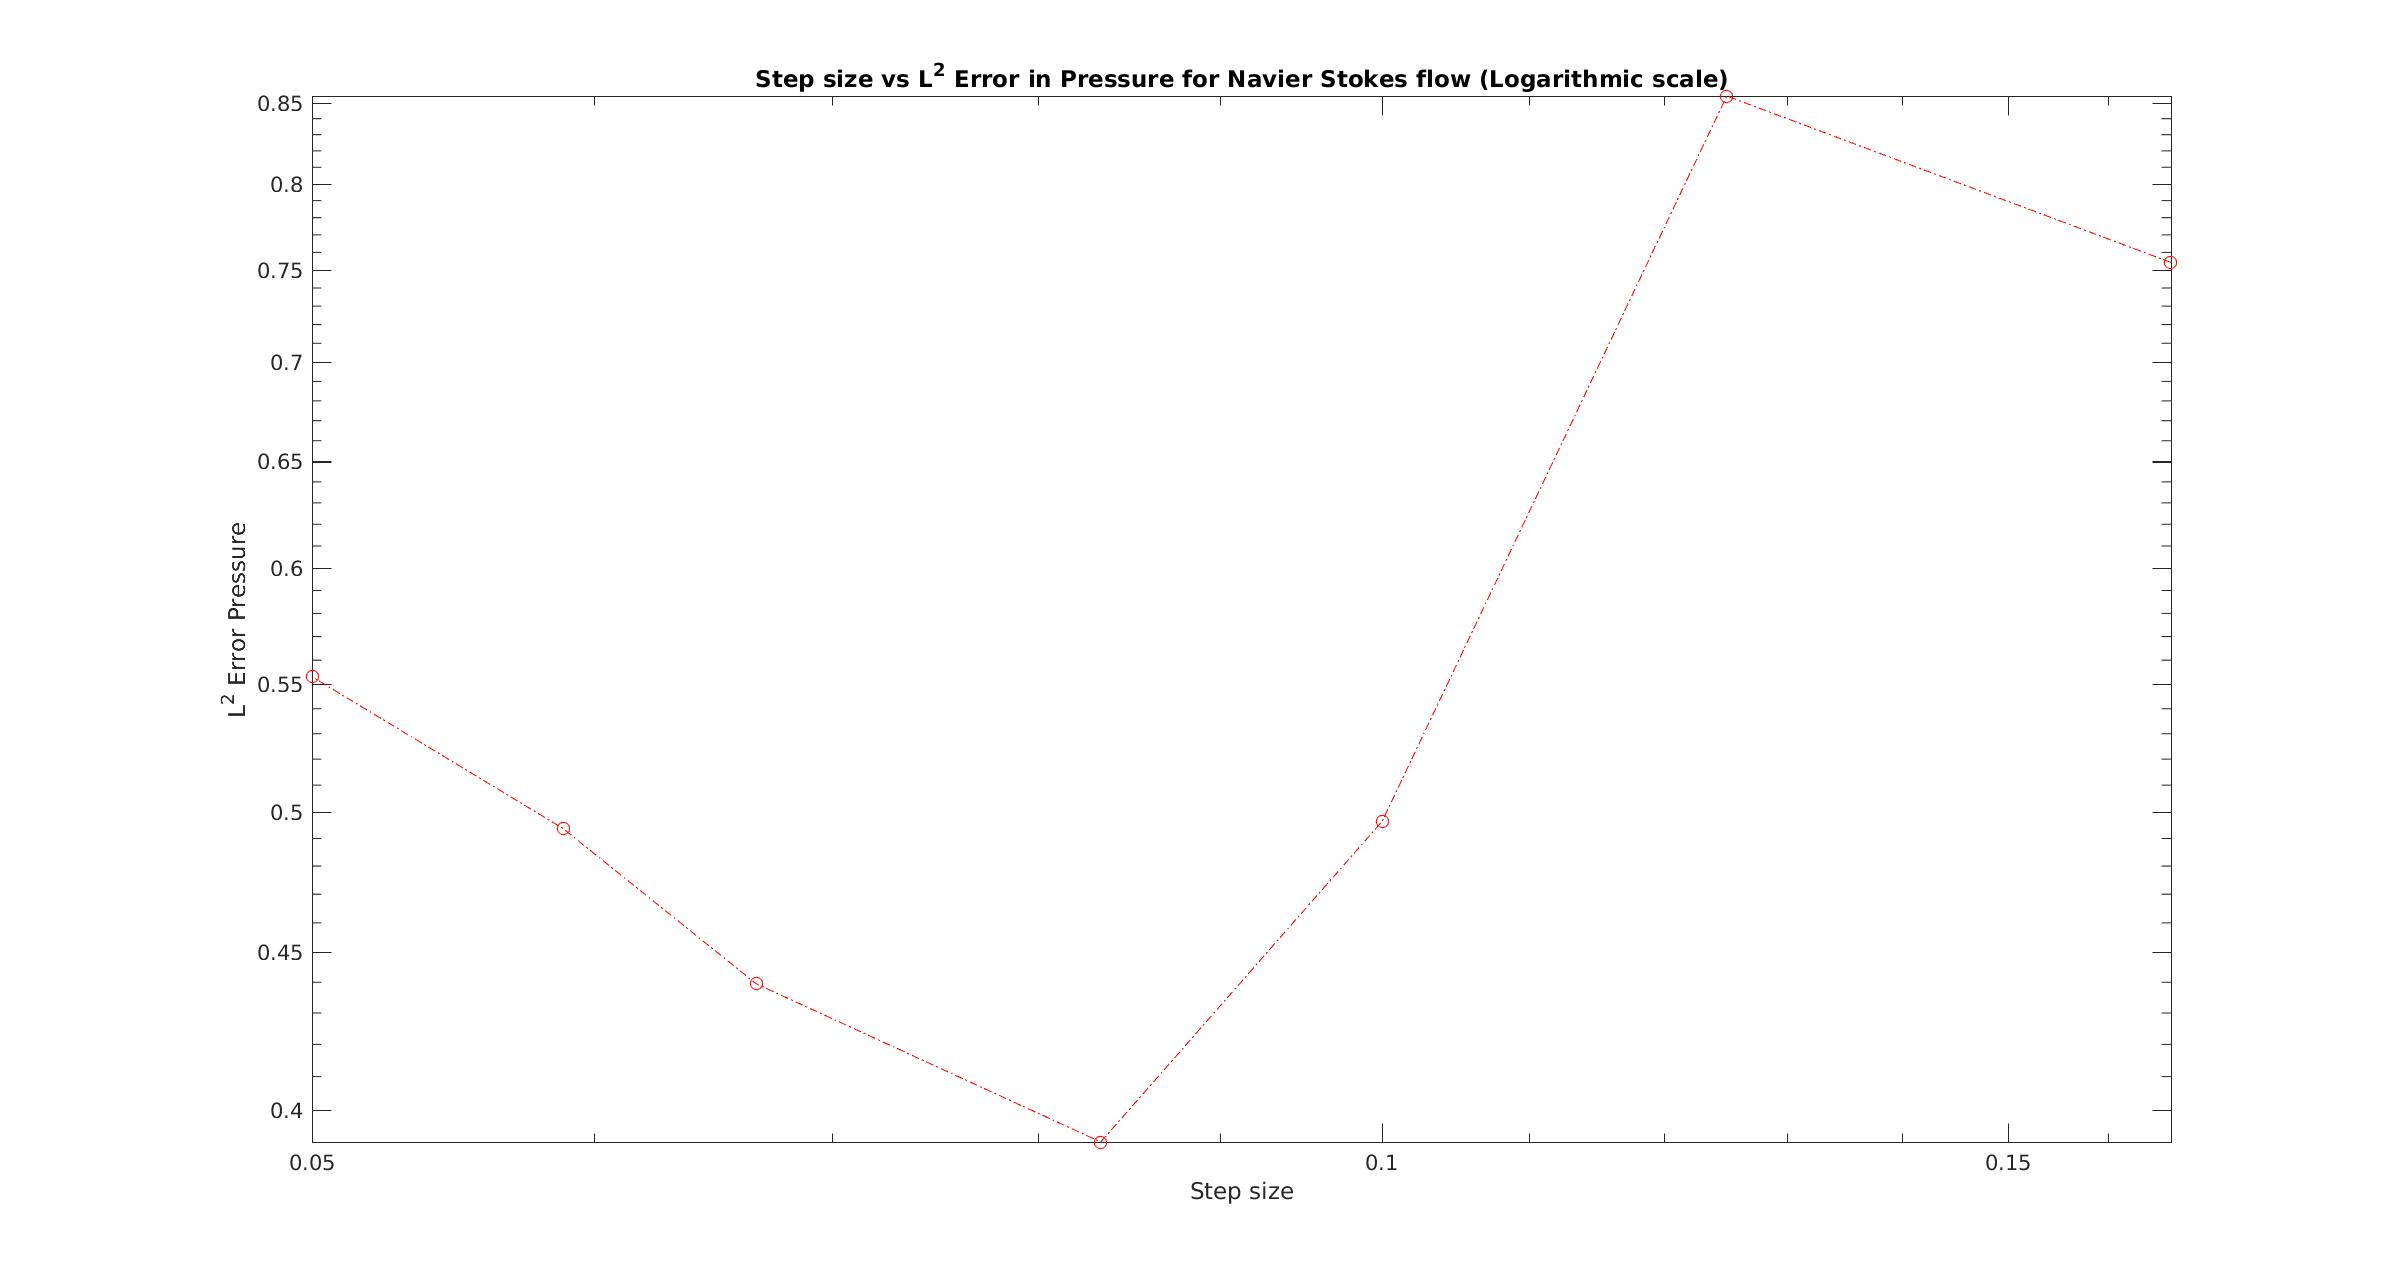
\includegraphics[width=\linewidth]{L2_convergence_pressure_n_s_log.jpg}
  \caption{$h-$convergence test for pressure in $L^2$ error (Logarithmic scale)}
  \label{fig:pre_navier_stoke_conv_log}
\end{subfigure}
\caption{$h-$convergence for the Navier Stokes flow in $L^2$ error (Logarithmic scale)}
\label{navier_stoke_conv_l2_log}
\end{figure}
\end{frame}
%------------------------------------------------
\begin{frame}
\frametitle{Navier-Stokes equation: Convergence test}
\begin{figure}
\begin{subfigure}{0.4\textwidth}	
  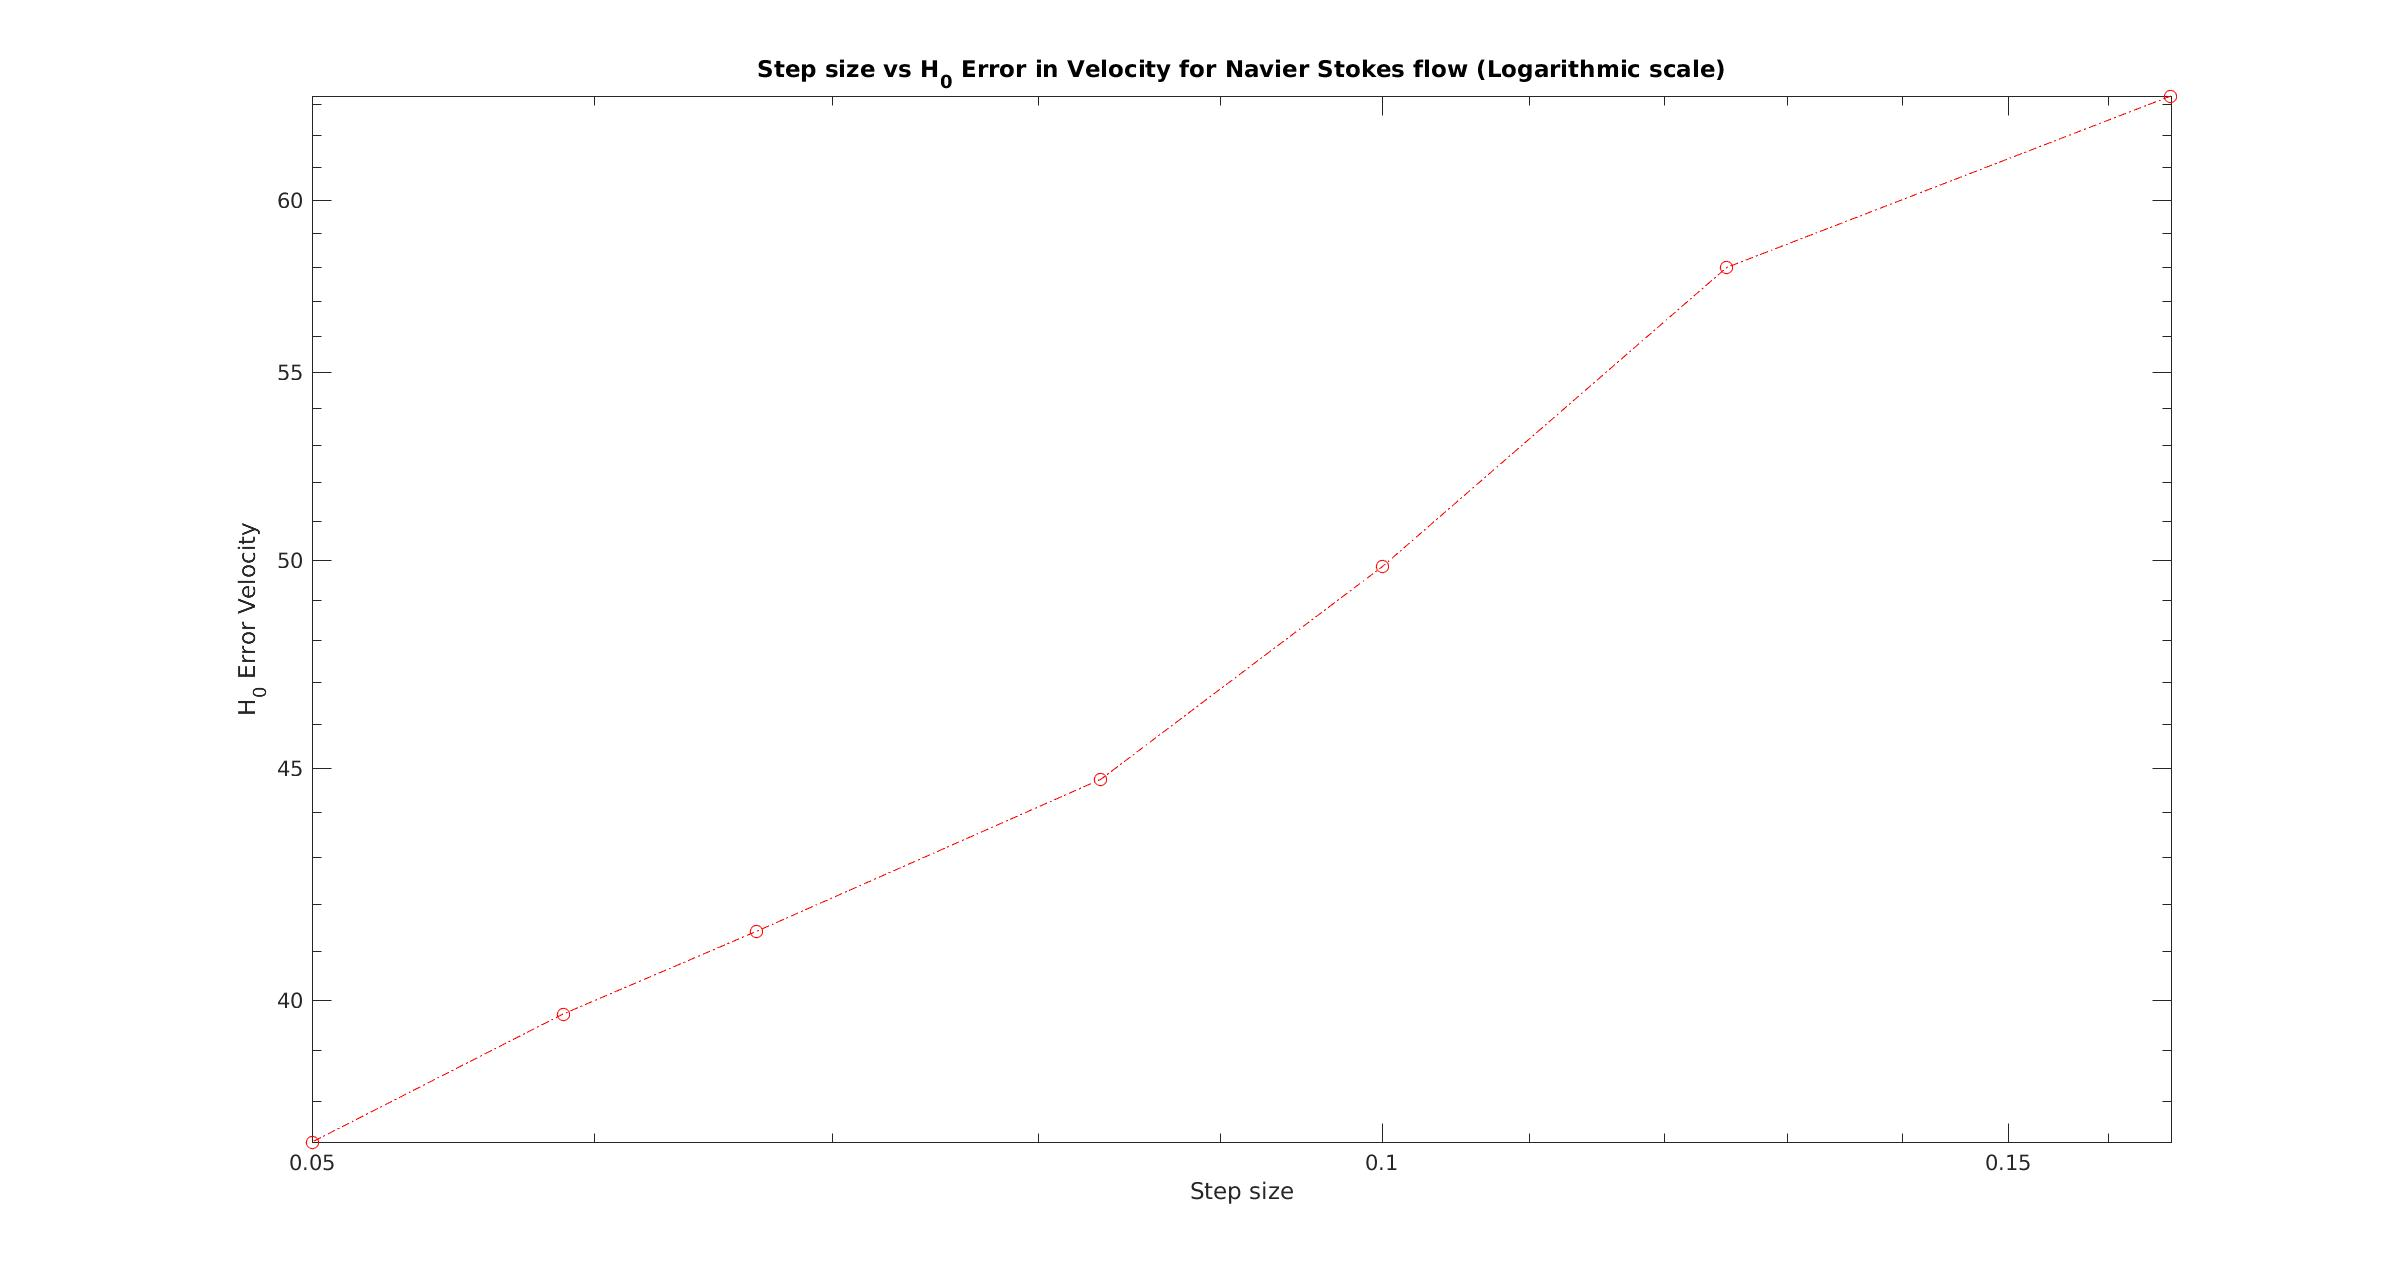
\includegraphics[width=\linewidth]{H0_convergence_velocity_n_s_log.jpg}
  \caption{$h-$convergence test for velocity $H_0$ error (logarithmic scale)}
  \label{fig:vel_navier_stoke_conv_log_h0}
\end{subfigure}
\begin{subfigure}{0.4\textwidth}	
  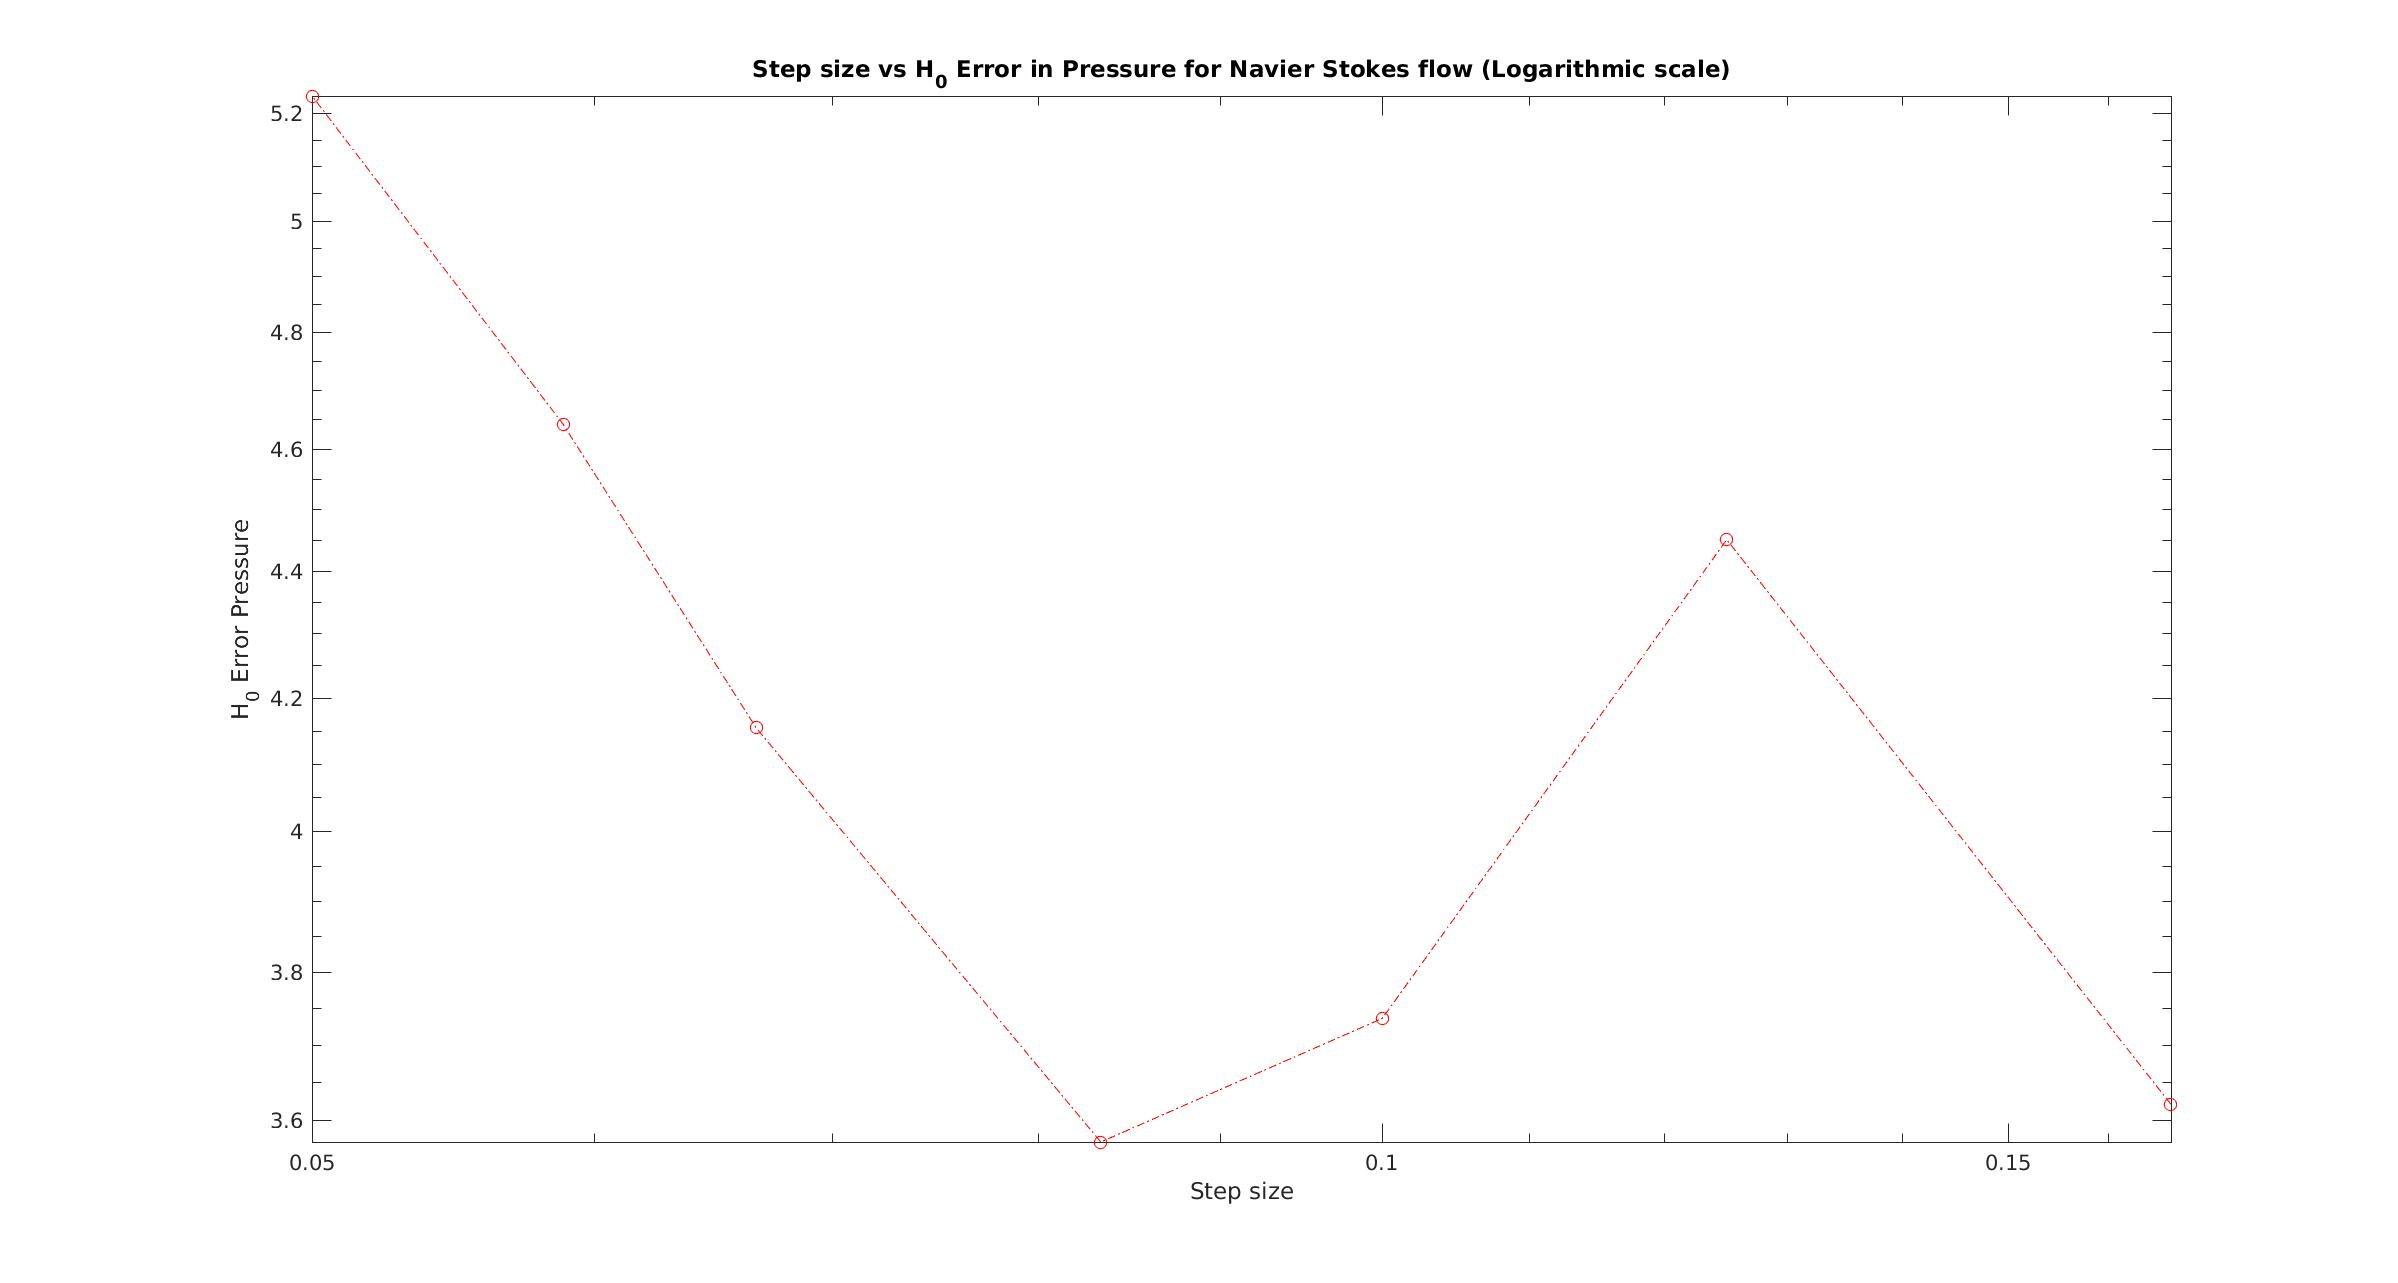
\includegraphics[width=\linewidth]{H0_convergence_pressure_n_s_log.jpg}
  \caption{$h-$convergence test for pressure in $H_0$ error (Logarithmic scale)}
  \label{fig:pre_navier_stoke_conv_log_h0}
\end{subfigure}
\caption{$h-$convergence for the Navier Stokes flow in $H_0$ error (Logarithmic scale)}
\label{navier_stoke_conv_h0_log}
\end{figure}
\end{frame}
%------------------------------------------------
\begin{frame}
\frametitle{Navier-Stokes equation: Flow around cylinder}
\begin{figure}
  \begin{subfigure}{0.3\textwidth}
    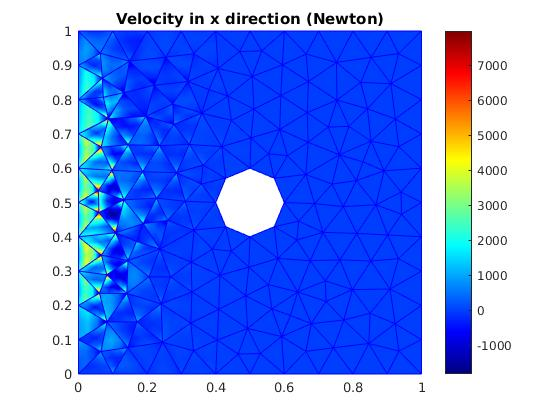
\includegraphics[width=\linewidth]{cylinder_newton_vx_bicgstab.jpg}
    \caption{$x-$velocity }
  \label{x_vel_navier_stoke_bicgstab}
  \end{subfigure}
  \begin{subfigure}{0.3\textwidth}
    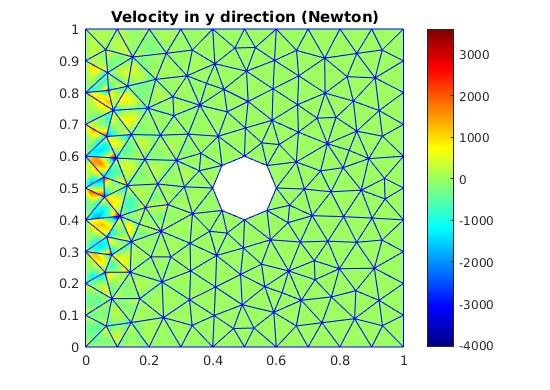
\includegraphics[width=\linewidth]{cylinder_newton_vy_bicgstab.jpg}
    \caption{$y-$velocity}
  \label{y_vel_navier_stoke_bicgstab}
  \end{subfigure}
  \begin{subfigure}{0.3\textwidth}
    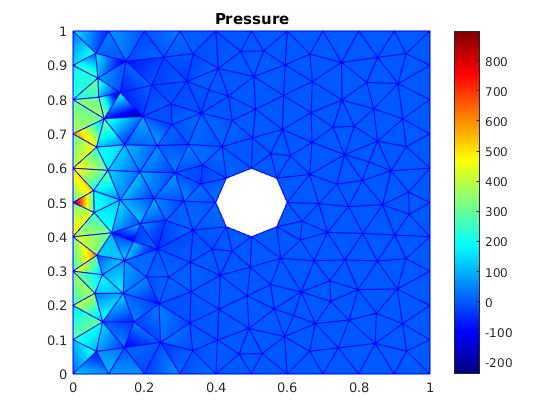
\includegraphics[width=\linewidth]{cylinder_newton_pressure_bicgstab.jpg}
    \caption{Pressure}
  \label{pressure_navier_stoke_bicgstab}
  \end{subfigure}
\caption{Flow over cylinder (Initial guess by $bicgstab$ solver)}
\label{flow_over_cylinder_bicgstab_n_s}
\end{figure}
\end{frame}
%------------------------------------------------
\begin{frame}
\frametitle{Navier-Stokes equation: Flow around cylinder}
\begin{figure}
  \begin{subfigure}{0.3\textwidth}
    \includegraphics[width=\linewidth]{cylinder_newton_vx_minres.jpg}
    \caption{$x-$velocity}
  \label{x_vel_navier_stoke_minres}
  \end{subfigure}
  \begin{subfigure}{0.3\textwidth}
    \includegraphics[width=\linewidth]{cylinder_newton_vy_minres.jpg}
    \caption{$y-$velocity}
  \label{y_vel_navier_stoke_minres}
  \end{subfigure}
  \begin{subfigure}{0.3\textwidth}
    \includegraphics[width=\linewidth]{cylinder_newton_pressure_minres.jpg}
    \caption{Pressure}
  \label{pressure_navier_stoke_minres}
  \end{subfigure}
\caption{Flow over cylinder (Initial guess by minres solver)}
\label{flow_over_cylinder_minres_n_s}
\end{figure}
\end{frame}
%------------------------------------------------
\begin{frame}
\frametitle{Navier-Stokes equation: Lid driven cavity}
\begin{itemize}
\item Domain: unit square [0,1] $\times$ [0,1].
\item Boundaries ${x = 0}, {x = 1}$ and ${y = 0}$, we impose no slip or zero velocity Dirichlet condition. 
\item On ${y = 1}$, we impose Dirichlet condition with Dirichlet velocity,
\begin{equation}
\begin{split}
u = a*(10x,0) \quad \textrm{for} \quad 0 \leq x \leq 0.1 \textrm{,}\\
u = a*(1,0) \quad \textrm{for} \quad 0.1 \leq x \leq 0.9 \textrm{,}\\
u = a*(10 - 10x,0) \quad \textrm{for} \quad 0.9 \leq x \leq 1 \textrm{.}
\end{split}
\end{equation}
\end{itemize}
\end{frame}
%------------------------------------------------
\begin{frame}
\frametitle{Navier-Stokes equation: Flow around cylinder}
\begin{itemize}
\item Domain: [0,1] $\times$ [0,1] with a cut out cylinder of diameter 0.2 centered at $(0.5,0.5)$.
\item The boundary ${x=0}$ is Dirichlet boundary with inflow velocity at point $(0,y)$ as $u = a*(y(1-y), 0)$. 
\item The boundaries ${y = 0}$ and ${y = 1}$ are Dirichlet boundaries with no slip or zero velocity condition. The boundary ${x = 1}$ is a Neumann boundary with zero Neumann value i.e. $t = (0, 0)$. 
\item The source term is $f = (0, 0)$.
\end{itemize}
\end{frame}
%------------------------------------------------


\end{document} \grid